\documentclass[11pt]{article}
\usepackage[margin=1in]{geometry}
\usepackage{amsmath,amssymb}
\DeclareMathOperator{\se}{\textrm{se}}
\usepackage{graphicx}
\usepackage{grffile} % better for finding image extensions
\usepackage[hidelinks]{hyperref}
\usepackage{breakurl}
\usepackage{xspace}
\title{Supplementary Tables and Figures}
\author{Anqi Zhu$^\dagger$, Nana Matoba$^\dagger$, Emmaleigh Wilson, Amanda L. Tapia,
  \\ Yun Li, Joseph G. Ibrahim, Jason L. Stein, Michael I. Love}

% now supplementary tables and figures
\setcounter{table}{0}
\renewcommand{\tablename}{Supplementary Table}

\setcounter{figure}{0}
\renewcommand{\figurename}{Supplementary Figure}

\newcommand{\Ncase}{$N_{\textrm{case}}$\xspace}
\newcommand{\Ncontrol}{$N_{\textrm{control}}$\xspace}

\begin{document}

\maketitle

\section*{Supplementary Tables}

\begin{table}[!ht]
\centering
\footnotesize
\begin{tabular}{r p{4in}}
eQTL Tissue & Resource \\
\hline
Artery Tibial (GTEx v8) & \url{https://console.cloud.google.com/storage/browser/gtex-resources} \\
Blood (eQTLGen 2019-12-23 release) & \url{https://www.eqtlgen.org/cis-eqtls.html} \\
Liver & \url{https://www.nature.com/articles/s41598-018-24219-z} \\
& \\
GWAS Phenotype & Resource \\
\hline
CAD (CARDIoGRAMplusC4D) & \url{http://www.cardiogramplusc4d.org/media/cardiogramplusc4d-consortium/data-downloads/cad.additive.Oct2015.pub.zip} \\
HDL (UKBB) & \url{https://www.dropbox.com/s/65jisgxwbbdrkaw/30760_irnt.gwas.imputed_v3.both_sexes.tsv.bgz} \\
LDL (UKBB) & \url{https://www.dropbox.com/s/4rnjzczwjgs5pgl/30780_irnt.gwas.imputed_v3.both_sexes.tsv.bgz} \\
\end{tabular}
\caption{Links to URLs for eQTL and GWAS summary data employed in
  MRLocus real data evaluation.}
\end{table}

\clearpage

\section*{Supplementary Figures}

\begin{figure}[!ht]
  \centering
  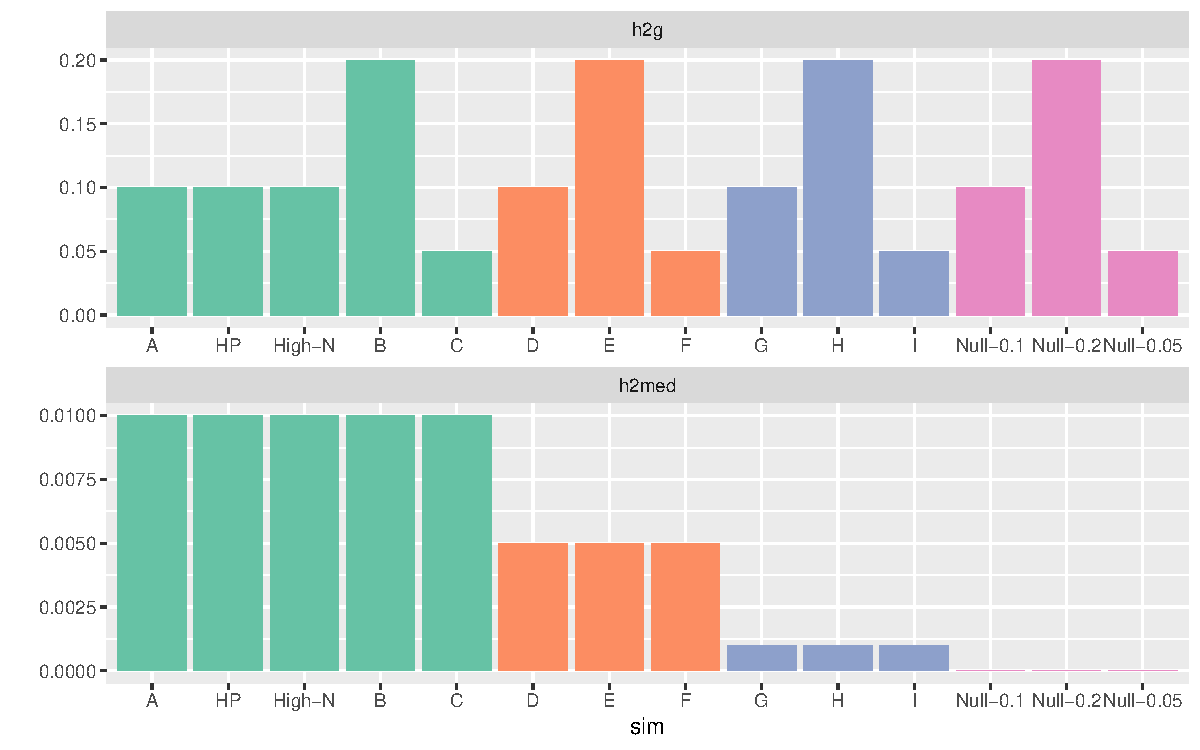
\includegraphics[width=.7\textwidth]{figs/sim_types}
  \caption{Diagram of the 12 types of \texttt{twas\_sim} simulations
    performed, varying eQTL $h^2$ (top row) and trait variance explained
    through gene expression (bottom row), with 20 replicates of each
    setting resulting in 240 simulations total. Results for simulation
    A are presented in Figure 2 in the main text, while results for
    the remaining 11 simulation settings follow in Supplementary
    Figures.}
\end{figure}

\begin{figure}[!ht]
  \centering
  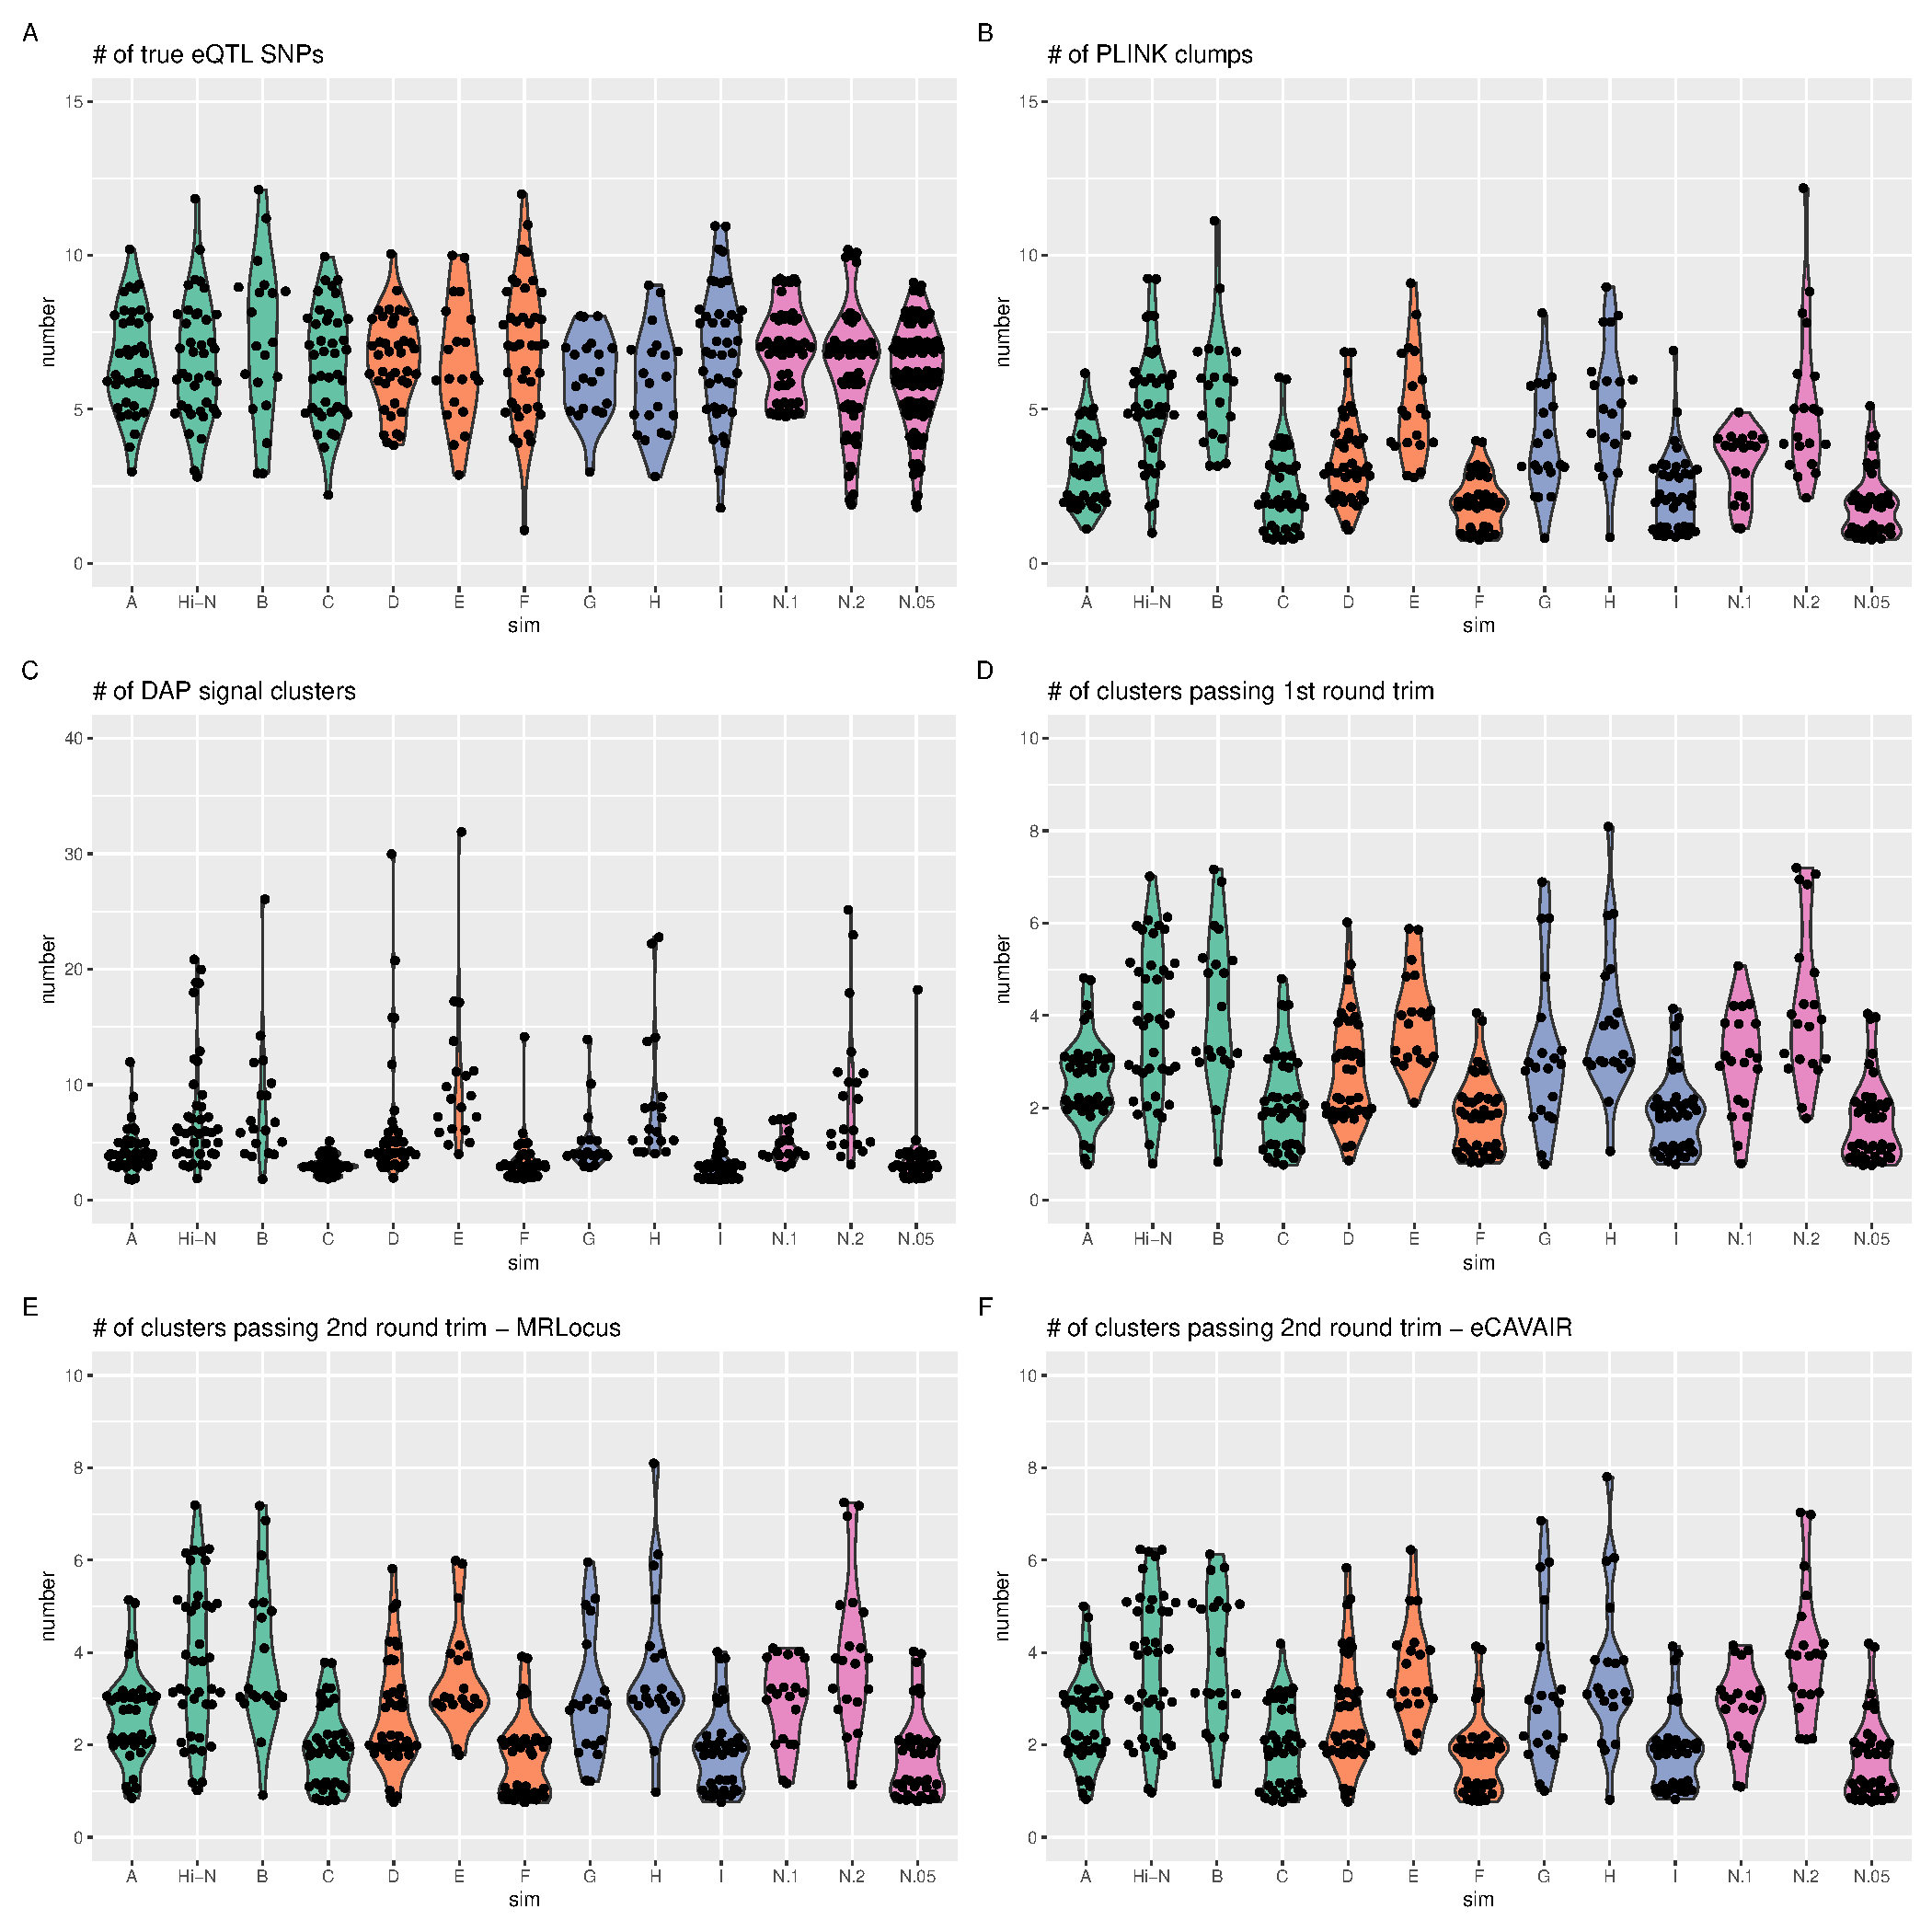
\includegraphics[width=\textwidth]{figs/sim_details}
  \caption{Number of (A) true causal eQTL SNPs, (B) PLINK clumps, 
    (C) DAP signal clusters per simulation, and number of clusters
    passing (D) 1st round LD trimming, (E) 2nd round LD trimming for
    MRLocus colocalization, and (F) 2nd round LD trimming for eCAVIAR
    colocalization.}
\end{figure}

\begin{figure}[!ht]
  \centering
  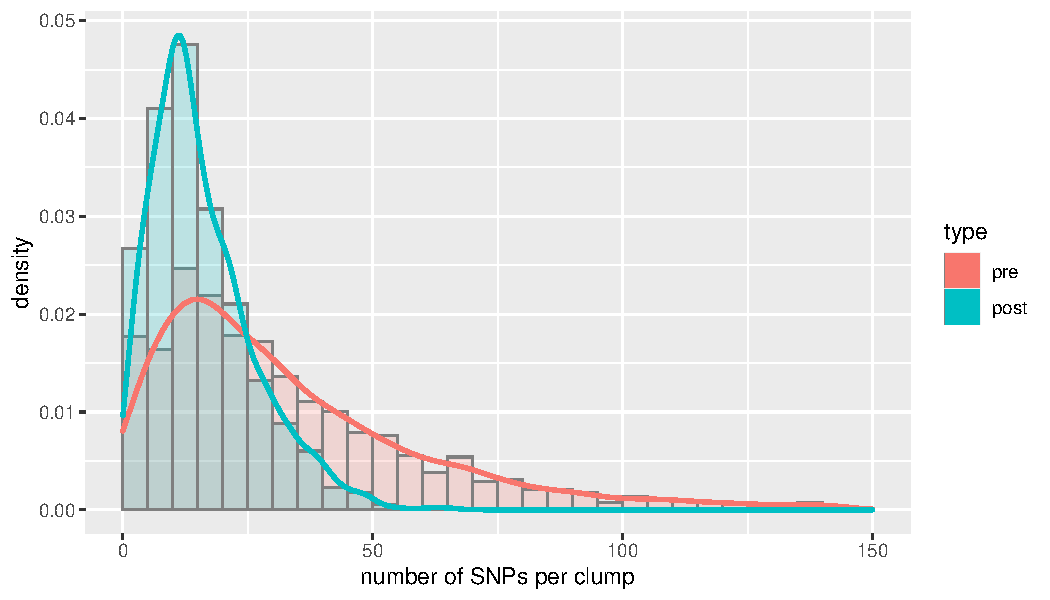
\includegraphics[width=.7\textwidth]{figs/snps_per_clump}
  \caption{SNPs per clump in the 240 simulations, before and after
    collapsing with MRLocus’ \texttt{collapseHighCorSNPs}
    function. The mean number of SNPs per clump was 19.9 and 8.8, and
    the median number of SNPs per clump was 15 and 8 (before and
    after, respectively).}
\end{figure}

\begin{figure}[!ht]
  \centering
  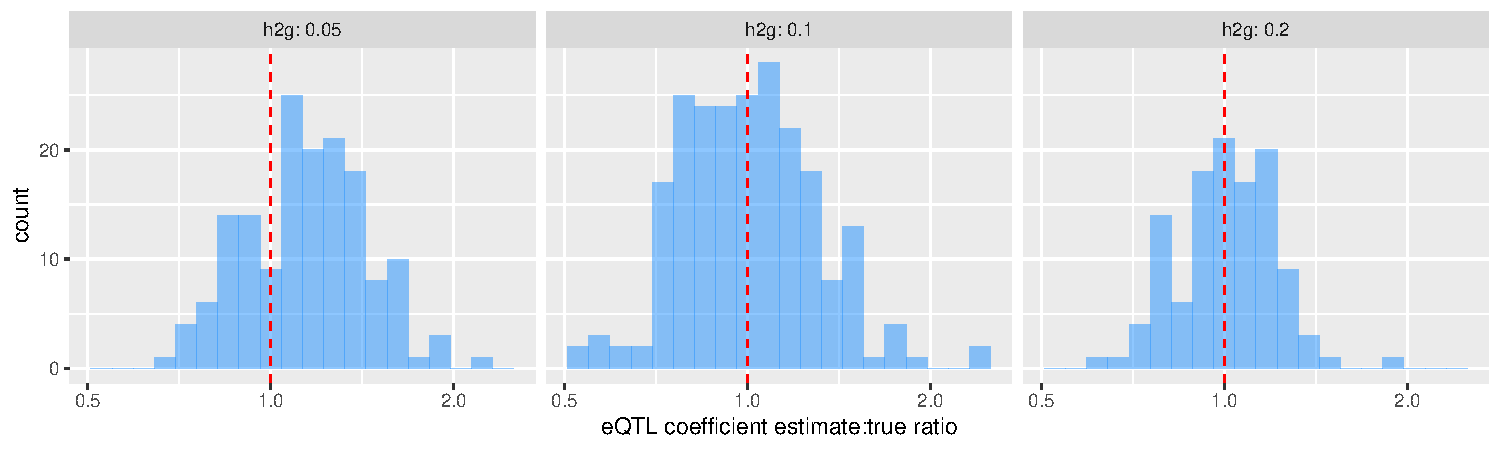
\includegraphics[width=\textwidth]{figs/sim_overest}
  \caption{Ratio of estimated eQTL coefficient over true value across
    simulations, grouped by h2g parameter. Histograms represent the
    ratio gor all causal eSNPs with un-adjusted eQTL p-value less than
    the clumping threshold (0.001).}
\end{figure}

\begin{figure}[!ht]
  \centering
  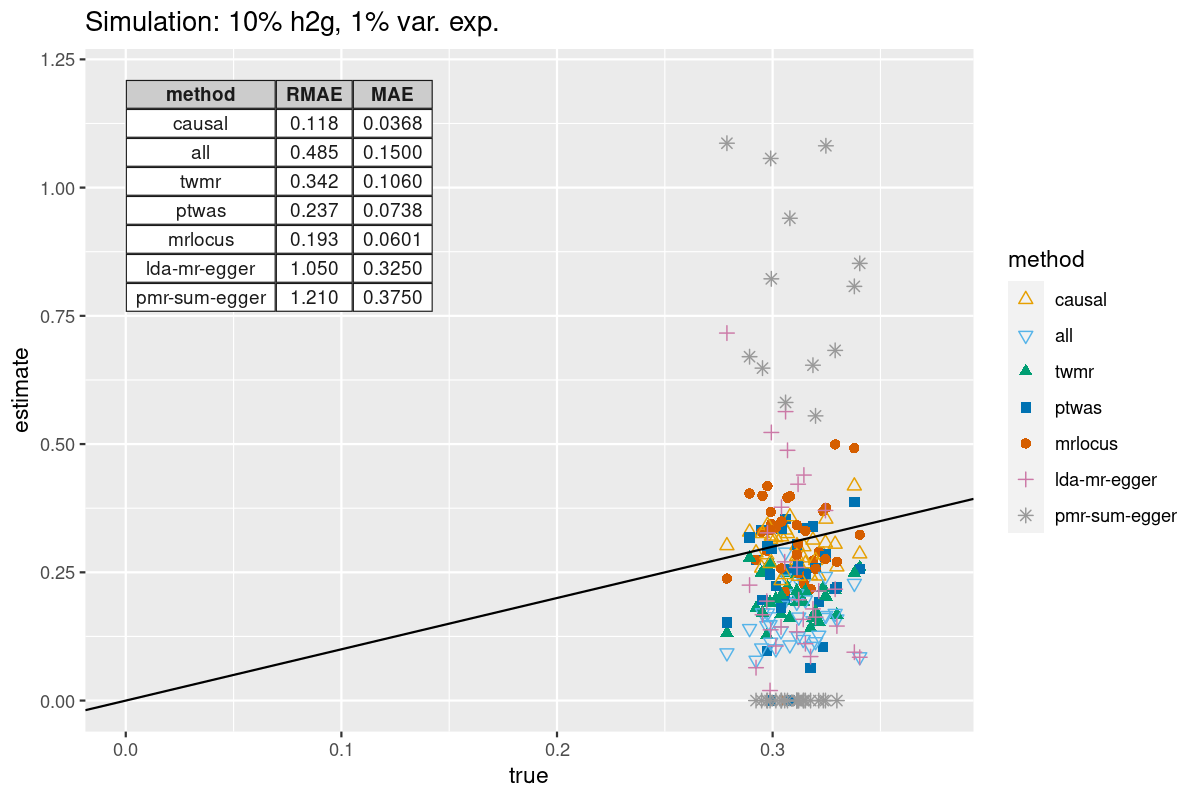
\includegraphics[width=.5\textwidth]{figs/sim1extra2.png}
  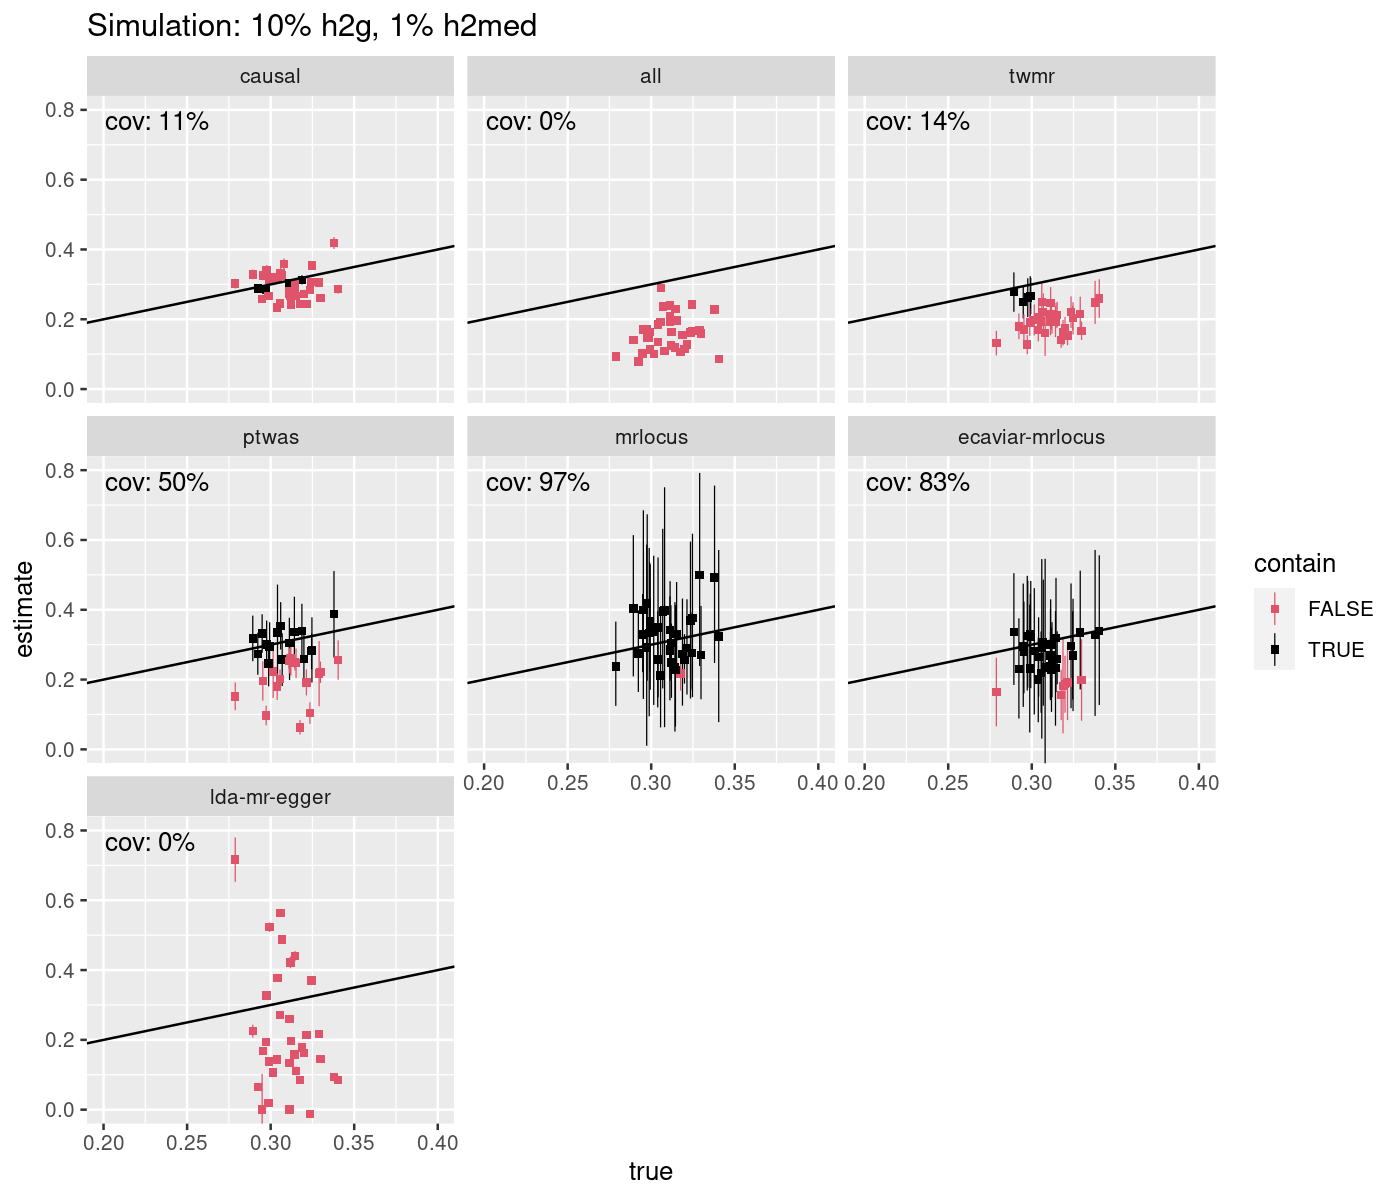
\includegraphics[width=.4\textwidth]{figs/cover1extra2.png}
  \caption{Accuracy and interval coverage of gene-to-trait effect
    estimation in simulation A, including LDA-MR-Egger and
    PMR-Summary-Egger in comparisons. As PMR-Summary-Egger does not
    provide a standard error for the causal effect, interval
    coverage was only computed for LDA-MR-Egger.}
\end{figure}

\begin{figure}[!ht]
  \centering
  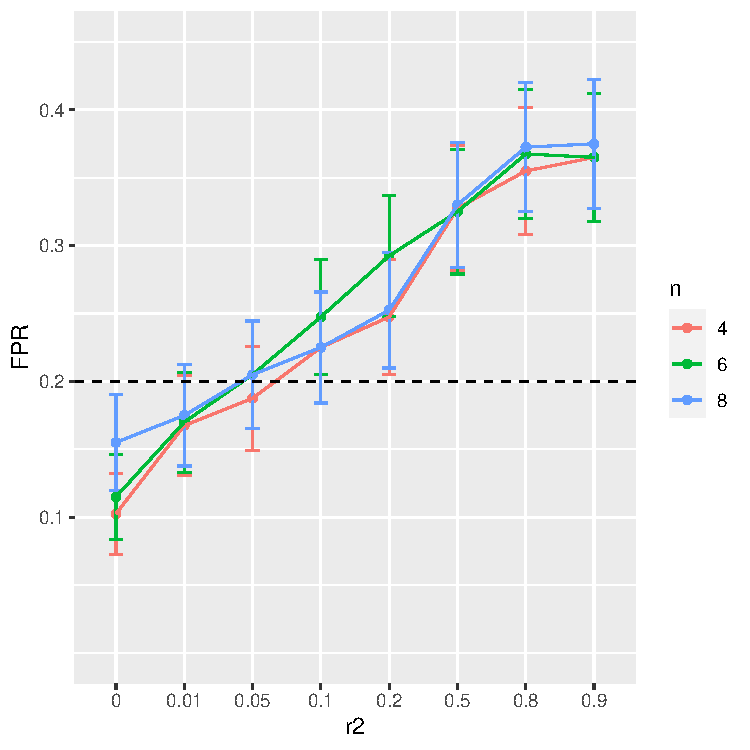
\includegraphics[width=.5\textwidth]{figs/corr_instr_sim}
  \caption{Assessment of the effect of correlated instruments on the
    false positive rate of MRLocus slope estimation. Increasing the
    $r^2$ of adjacent signal clusters raised the rate of 80\% credible
    intervals not covering the true value of the slope $\alpha =
    0$. The number of signal clusters was varied among $\{4,6,8\}$.}
\end{figure}

\begin{figure}[!ht]
  \centering
  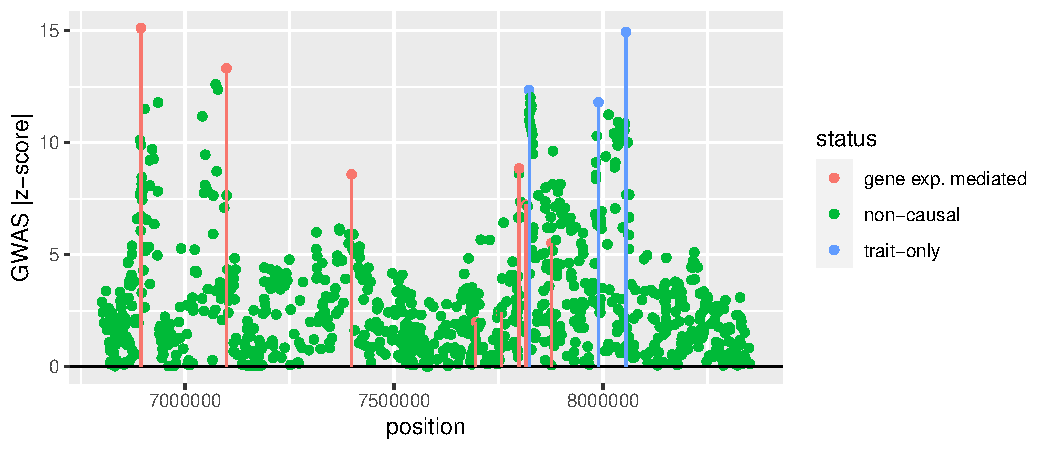
\includegraphics[width=.7\textwidth]{figs/hp_example}
  \caption{Example of one of the iterations of the simulation of
    partial mediation with horizontal pleiotropy (HP), where three
    large trait-only association signals are added to a simulation
    with $h^2g = 10\%$ and $h^2med = 1\%$. Absolute Z-scores for the
    GWAS population are calculated from estimated coefficients and
    their standard errors, and colored by the true status in the
    simulation.}
  \label{sf:hp}
\end{figure}

\begin{figure}[!ht]
  \centering
  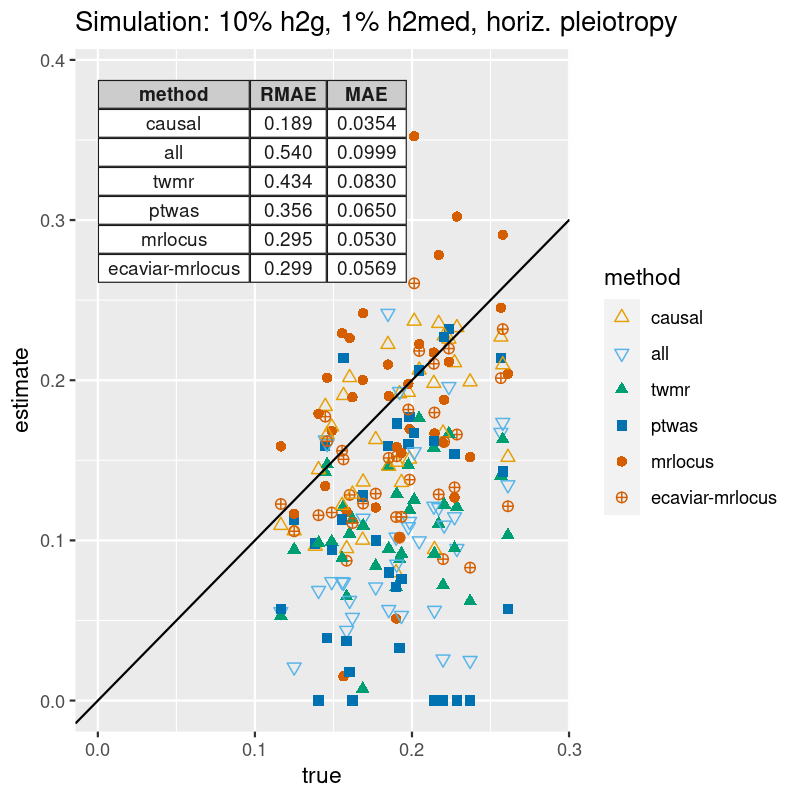
\includegraphics[width=.33\textwidth]{figs/simhp.png}
  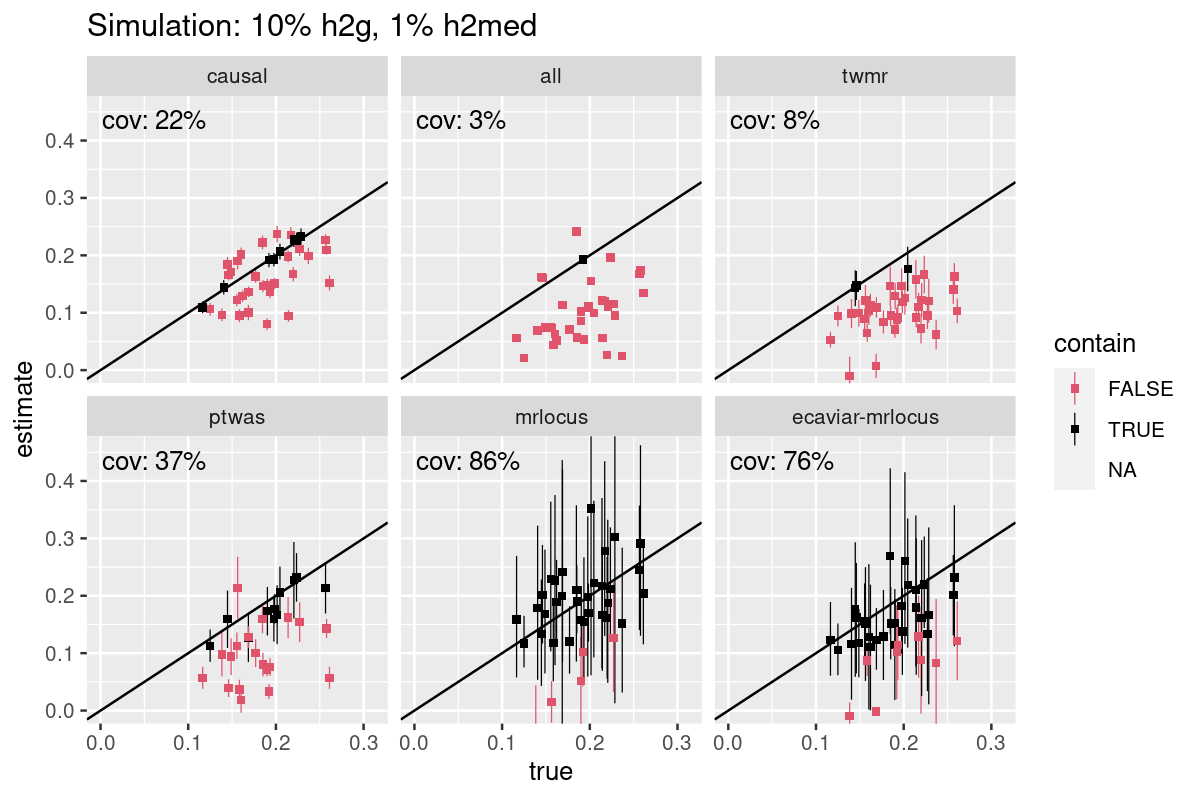
\includegraphics[width=.5\textwidth]{figs/coverhp.png}
  \caption{Accuracy and interval coverage of TWMR, PTWAS, MRLocus, and
  eCAVIAR-MRLocus on the simulation of partial mediation with
  horizontal pleiotropy (as in the example region in Supplementary
  Figure~\ref{sf:hp}).}
\end{figure}

\begin{figure}[!ht]
  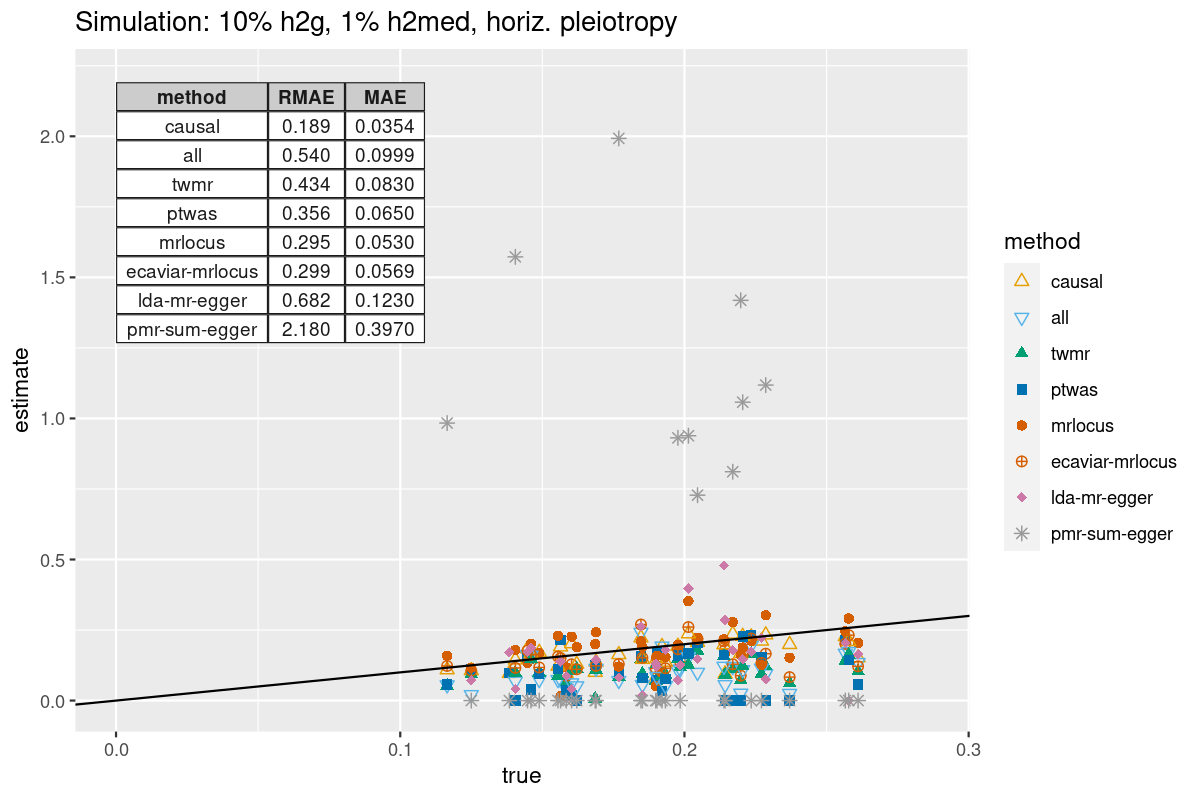
\includegraphics[width=.5\textwidth]{figs/simhpextra.png}
  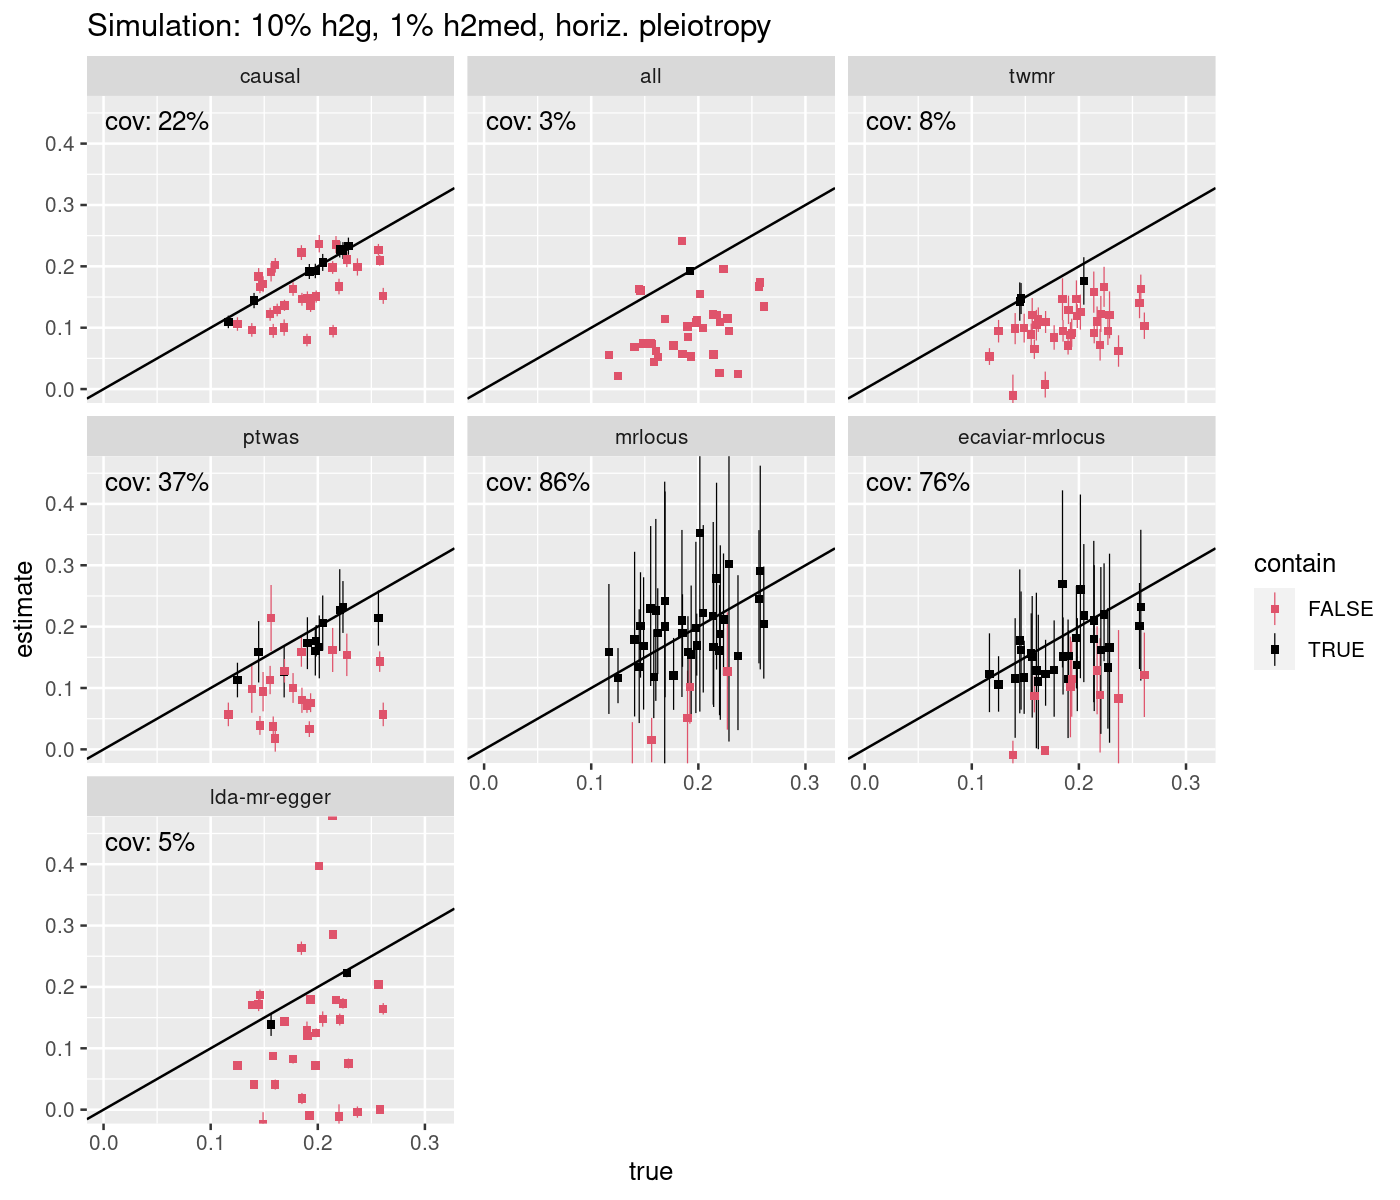
\includegraphics[width=.37\textwidth]{figs/coverhpextra.png}
  \caption{Accuracy and interval coverage of methods on the simulation
    of partial mediation with horizontal pleiotropy, including
    LDA-MR-Egger and PMR-Summary-Egger. As PMR-Summary-Egger does not
    provide a standard error for the causal effect, interval coverage
    was only computed for LDA-MR-Egger.}
\end{figure}

\begin{figure}[!ht]
  \centering
  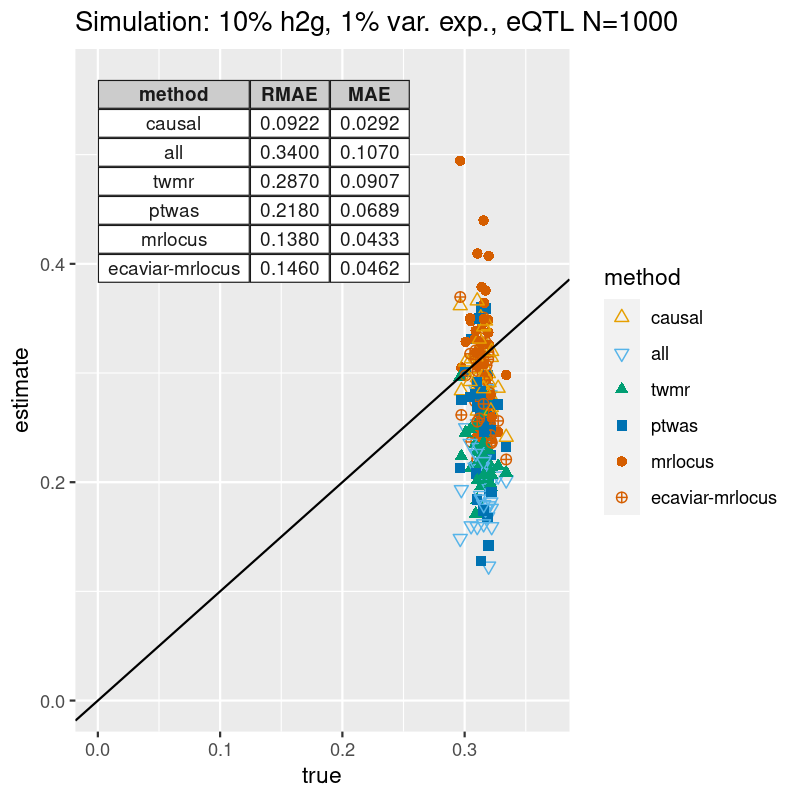
\includegraphics[width=.33\textwidth]{figs/simhigh_n.png}
  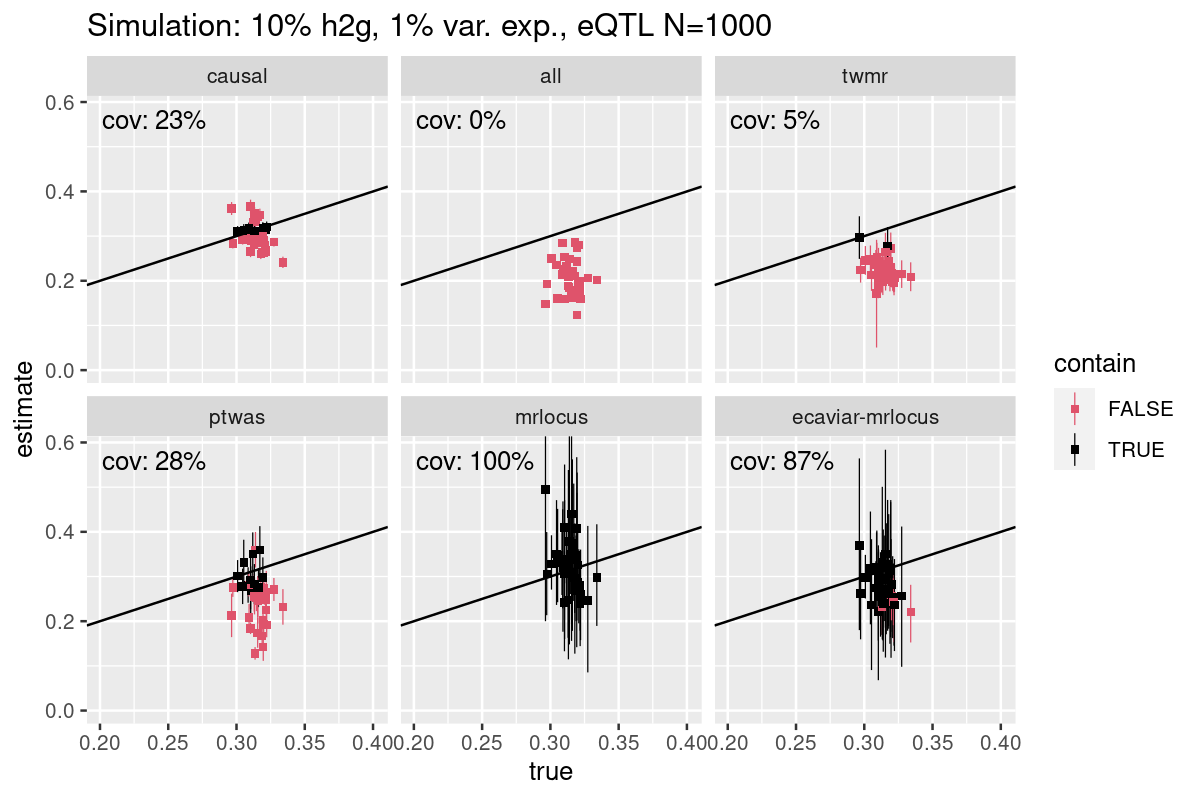
\includegraphics[width=.5\textwidth]{figs/coverhigh_n.png}
  \caption{Accuracy and interval coverage of TWMR, PTWAS, MRLocus, and
  eCAVIAR-MRLocus on the same simulation settings as simulation A but
  with increased $N_{\textrm{eQTL}} = 1000$ (instead of the default
  value $N_{\textrm{eQTL}} = 500$).}
\end{figure}

\begin{figure}[!ht]
  \centering
  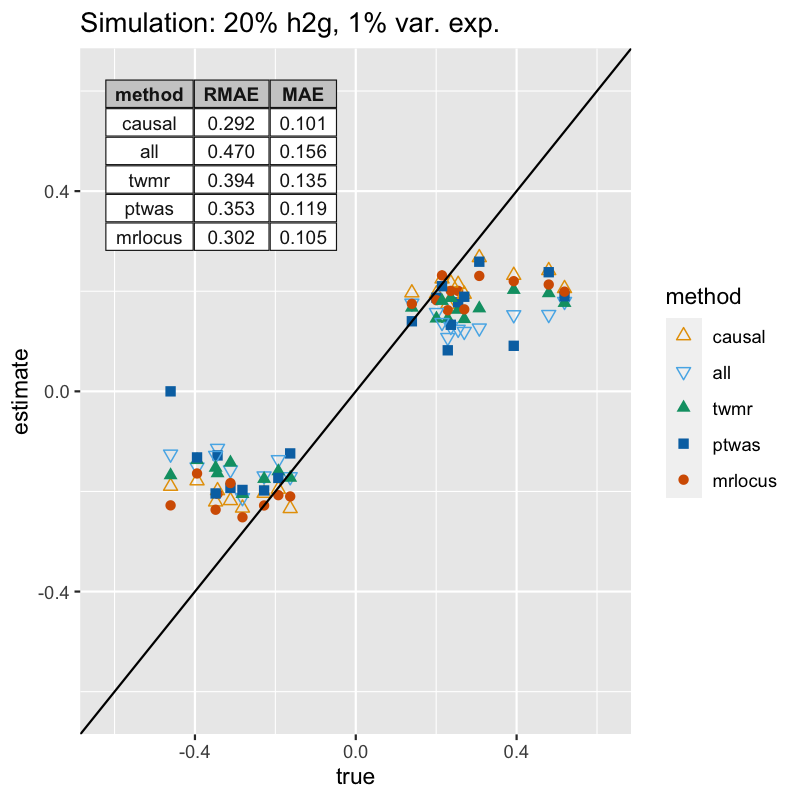
\includegraphics[width=.6\textwidth]{figs/sim3.png}
  \caption{Accuracy of gene-to-trait effect estimation in simulation B.}
\end{figure}

\begin{figure}[!ht]
  \centering
  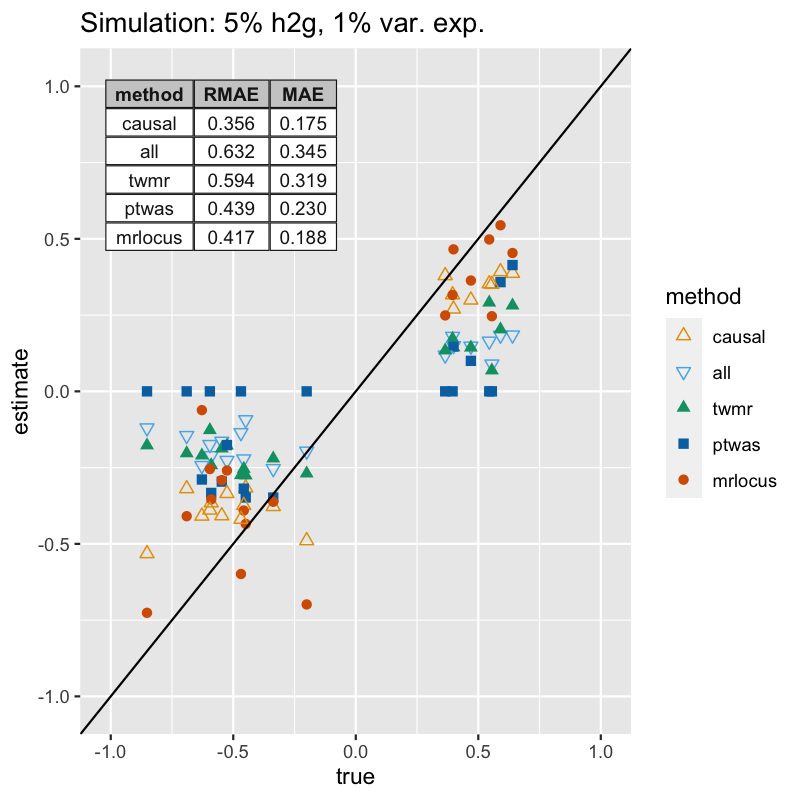
\includegraphics[width=.6\textwidth]{figs/sim2.png}
  \caption{Accuracy of gene-to-trait effect estimation in simulation C.}
\end{figure}

\begin{figure}[!ht]
  \centering
  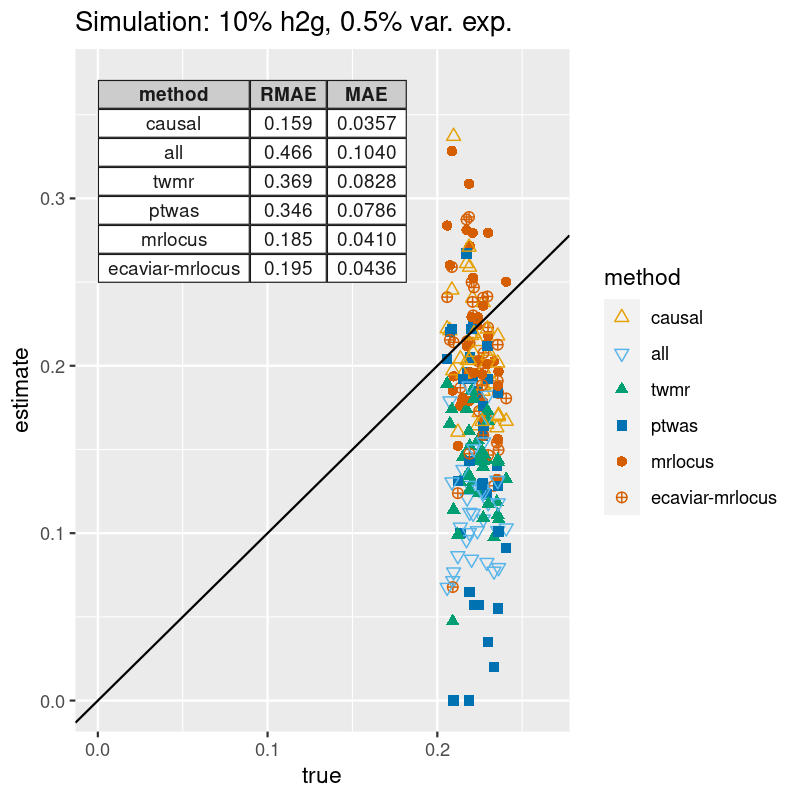
\includegraphics[width=.6\textwidth]{figs/sim4.png}
  \caption{Accuracy of gene-to-trait effect estimation in simulation D.}
\end{figure}

\begin{figure}[!ht]
  \centering
  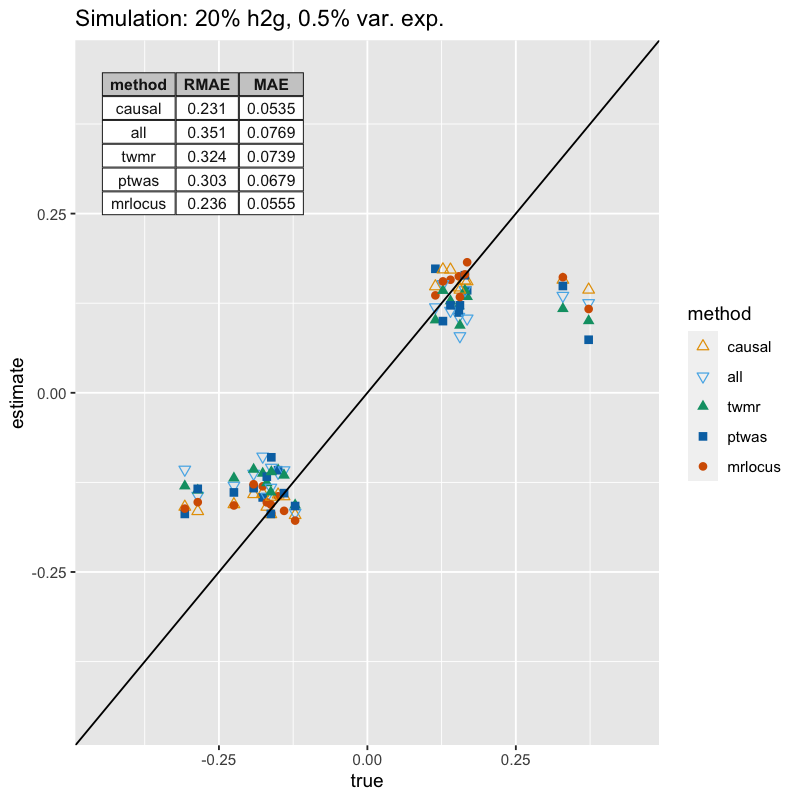
\includegraphics[width=.6\textwidth]{figs/sim6.png}
  \caption{Accuracy of gene-to-trait effect estimation in simulation E.}
\end{figure}

\begin{figure}[!ht]
  \centering
  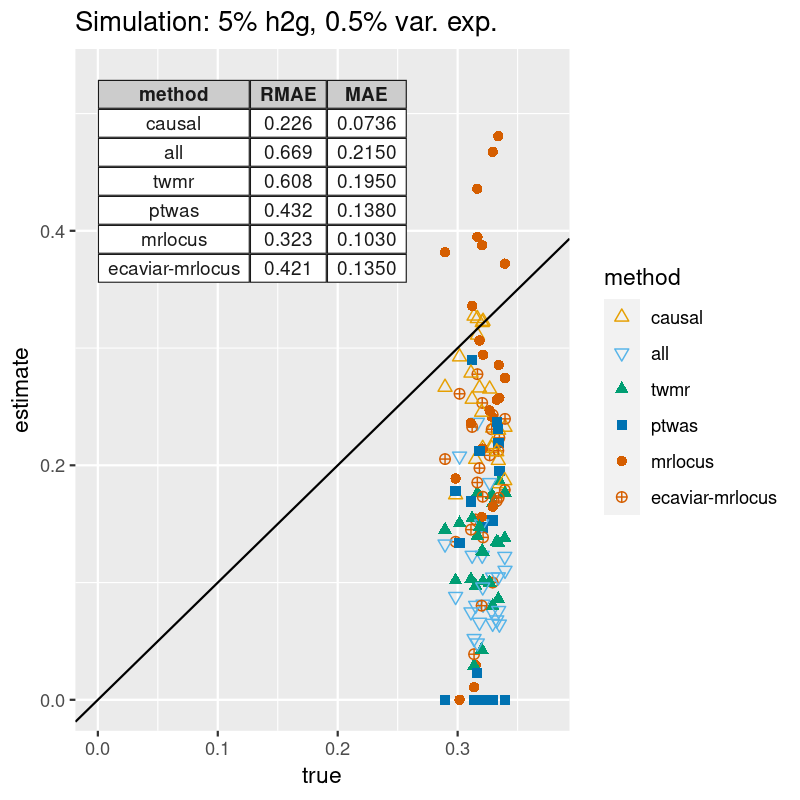
\includegraphics[width=.6\textwidth]{figs/sim8.png}
  \caption{Accuracy of gene-to-trait effect estimation in simulation F.}
\end{figure}

\begin{figure}[!ht]
  \centering
  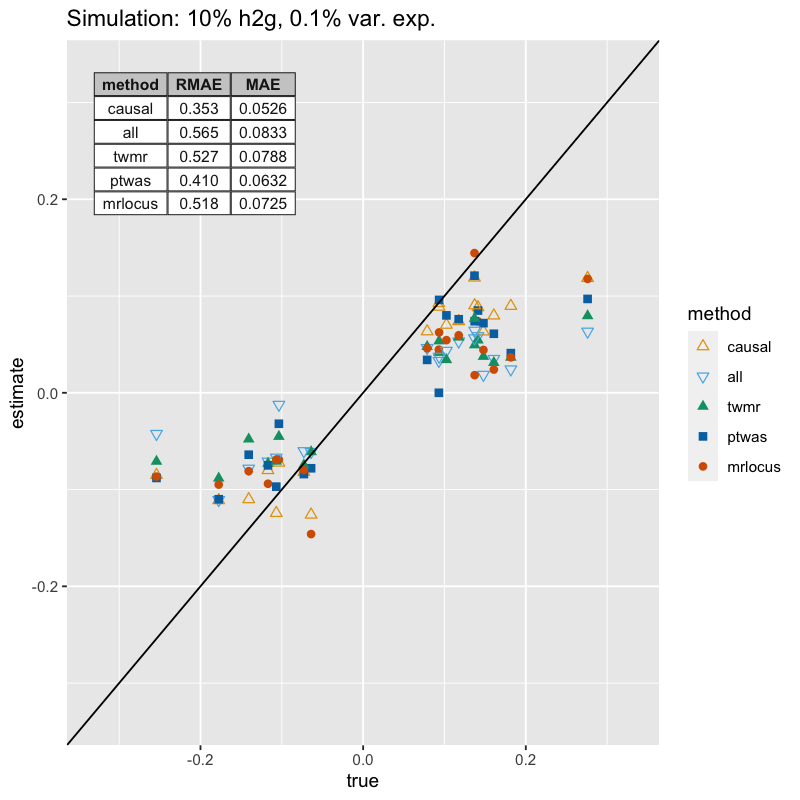
\includegraphics[width=.6\textwidth]{figs/sim5.png}
  \caption{Accuracy of gene-to-trait effect estimation in simulation G.}
\end{figure}

\begin{figure}[!ht]
  \centering
  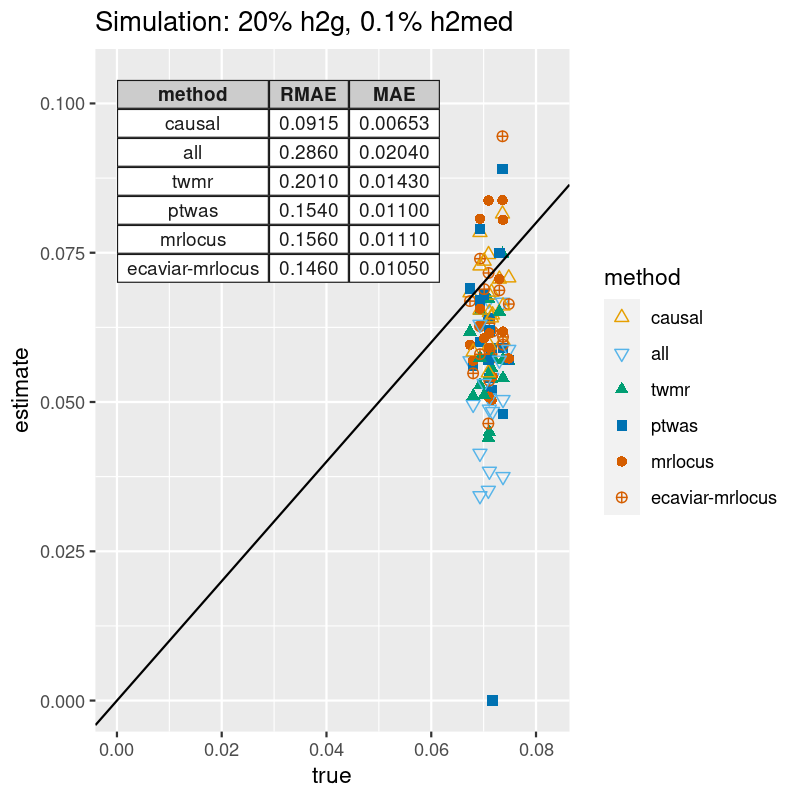
\includegraphics[width=.6\textwidth]{figs/sim7.png}
  \caption{Accuracy of gene-to-trait effect estimation in simulation H.}
\end{figure}

\begin{figure}[!ht]
  \centering
  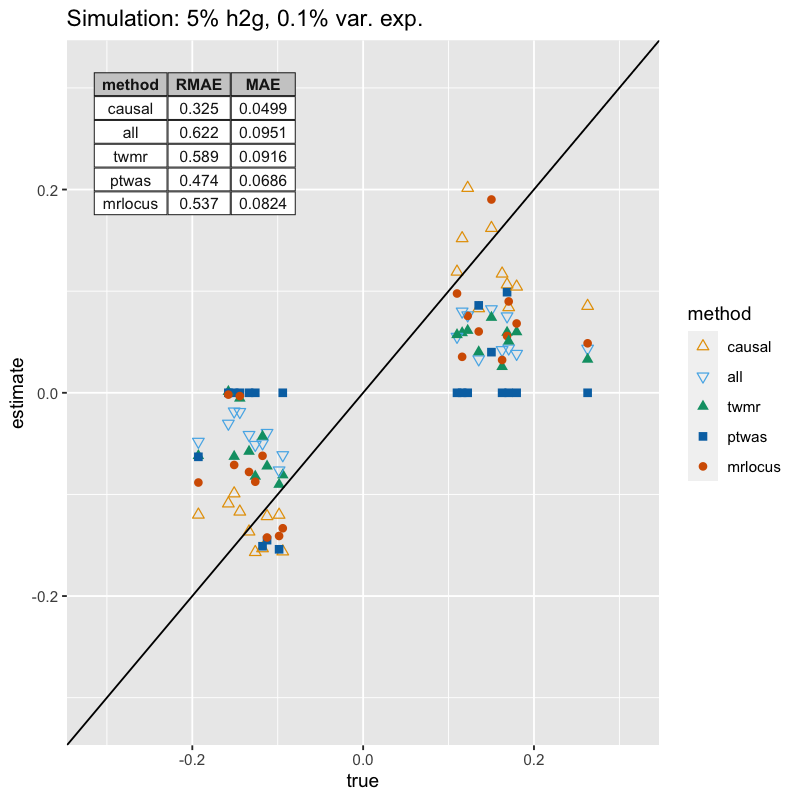
\includegraphics[width=.6\textwidth]{figs/sim9.png}
  \caption{Accuracy of gene-to-trait effect estimation in simulation I.}
\end{figure}

\begin{figure}[!ht]
  \centering
  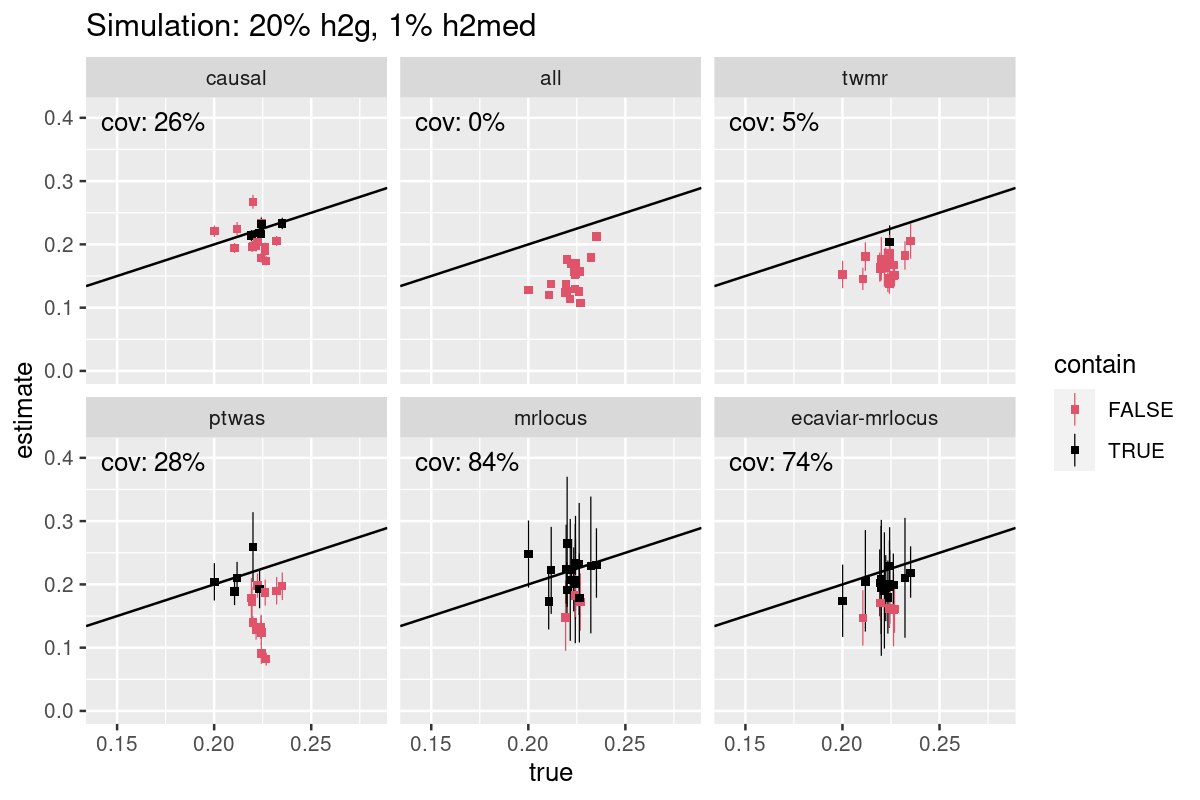
\includegraphics[width=.8\textwidth]{figs/cover3.png}
  \caption{Coverage of confidence or credible intervals for the
    gene-to-trait effect in simulation B.}
\end{figure}

\begin{figure}[!ht]
  \centering
  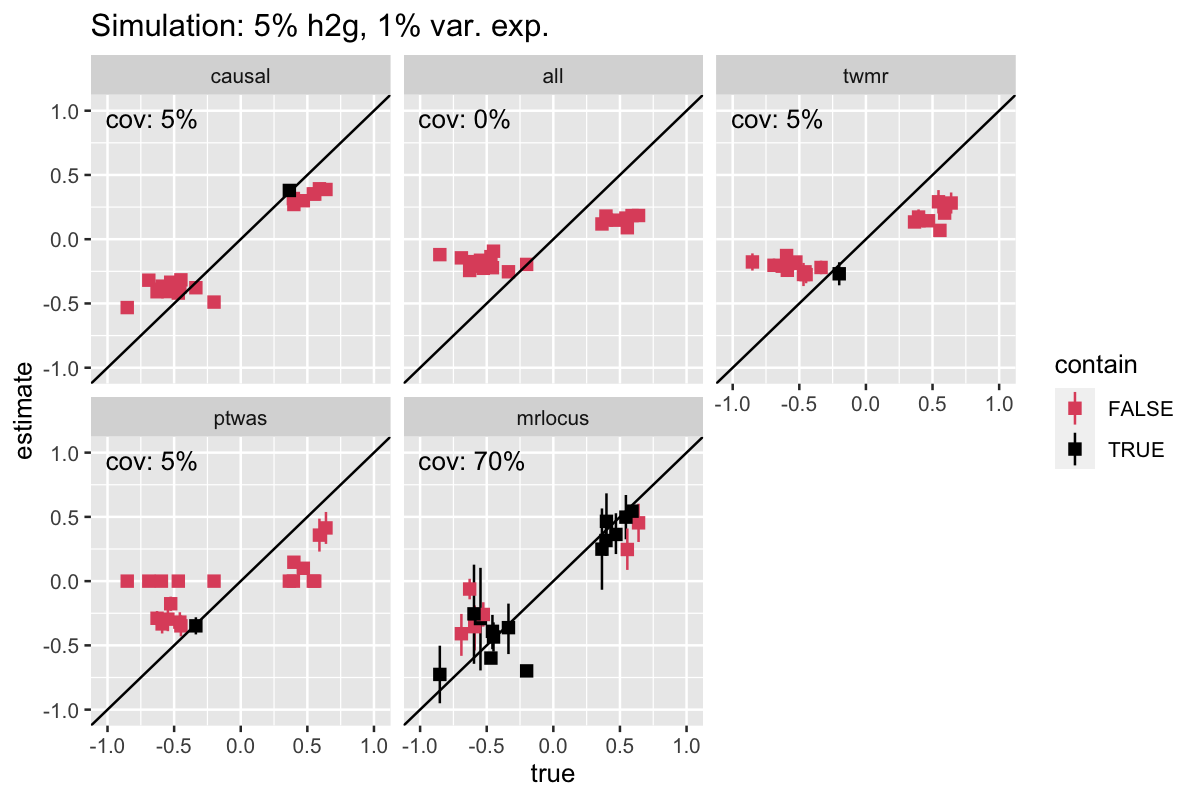
\includegraphics[width=.8\textwidth]{figs/cover2.png}
  \caption{Coverage of confidence or credible intervals for the
    gene-to-trait effect in simulation C.}
\end{figure}

\begin{figure}[!ht]
  \centering
  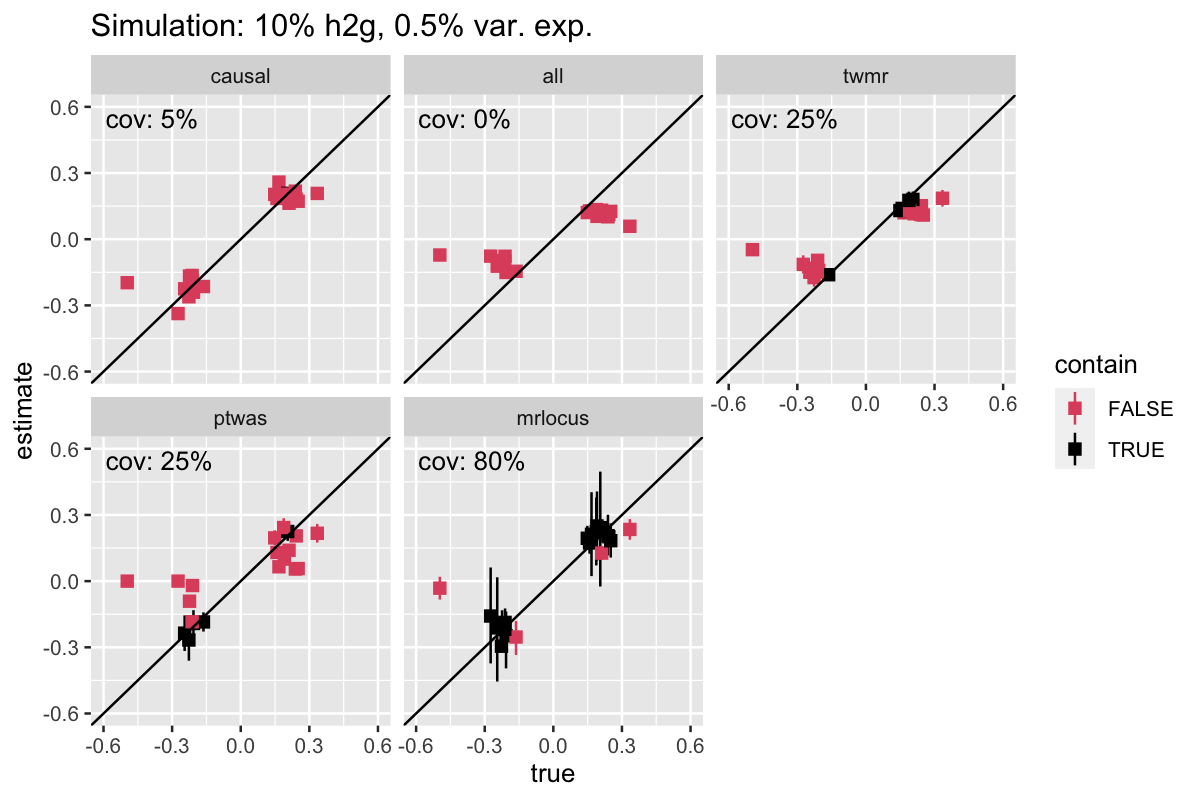
\includegraphics[width=.8\textwidth]{figs/cover4.png}
  \caption{Coverage of confidence or credible intervals for the
    gene-to-trait effect in simulation D.}
\end{figure}

\begin{figure}[!ht]
  \centering
  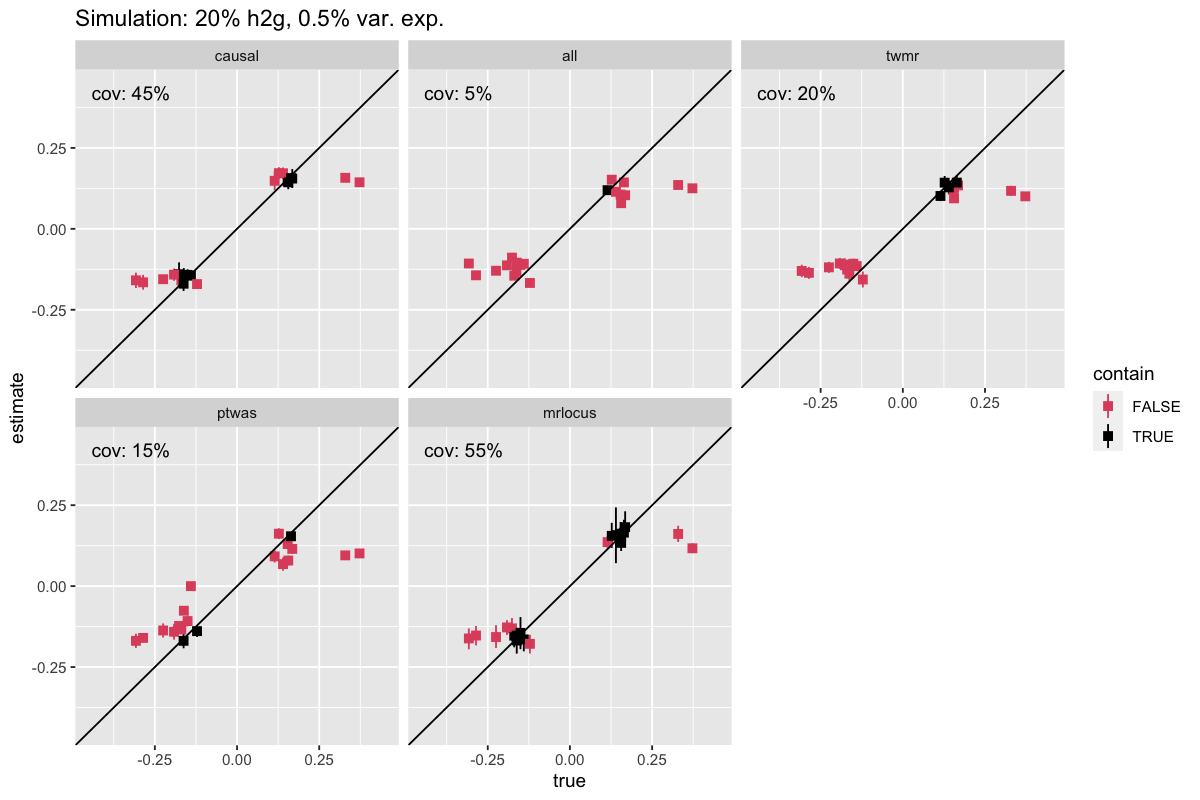
\includegraphics[width=.8\textwidth]{figs/cover6.png}
  \caption{Coverage of confidence or credible intervals for the
    gene-to-trait effect in simulation E.}
\end{figure}

\begin{figure}[!ht]
  \centering
  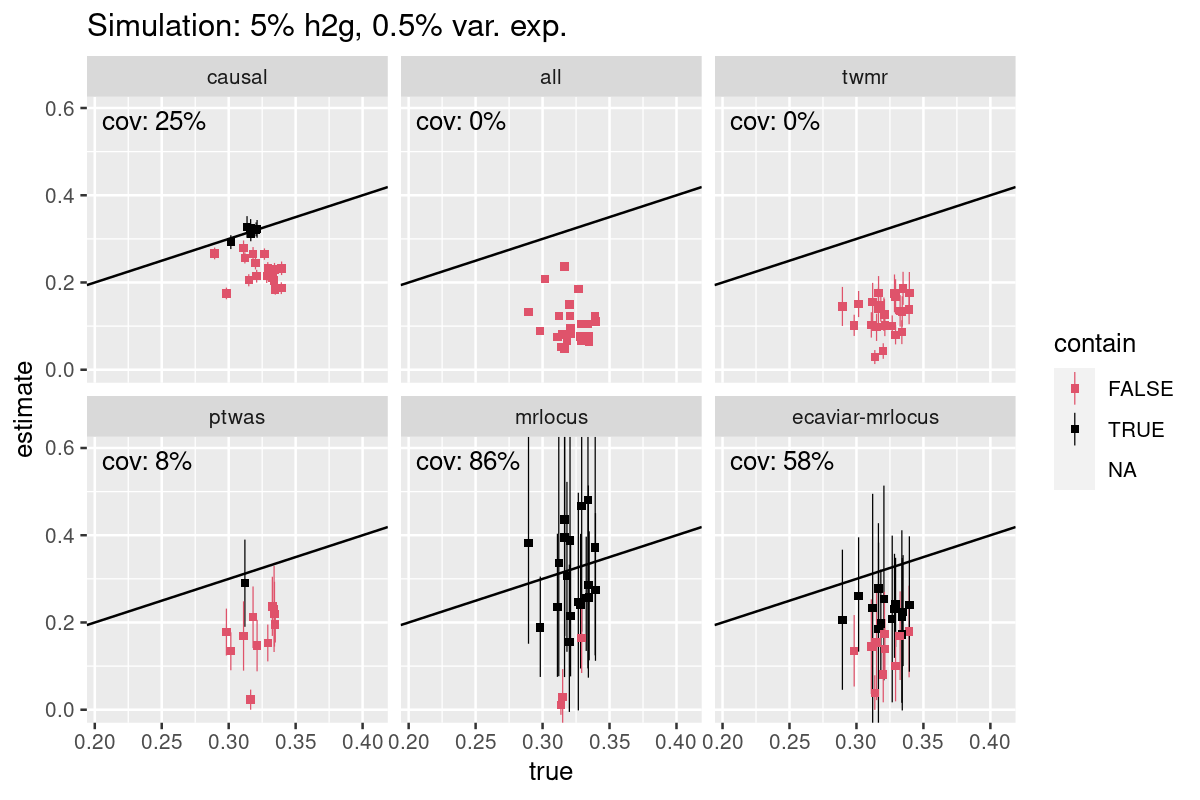
\includegraphics[width=.8\textwidth]{figs/cover8.png}
  \caption{Coverage of confidence or credible intervals for the
    gene-to-trait effect in simulation F.}
\end{figure}

\begin{figure}[!ht]
  \centering
  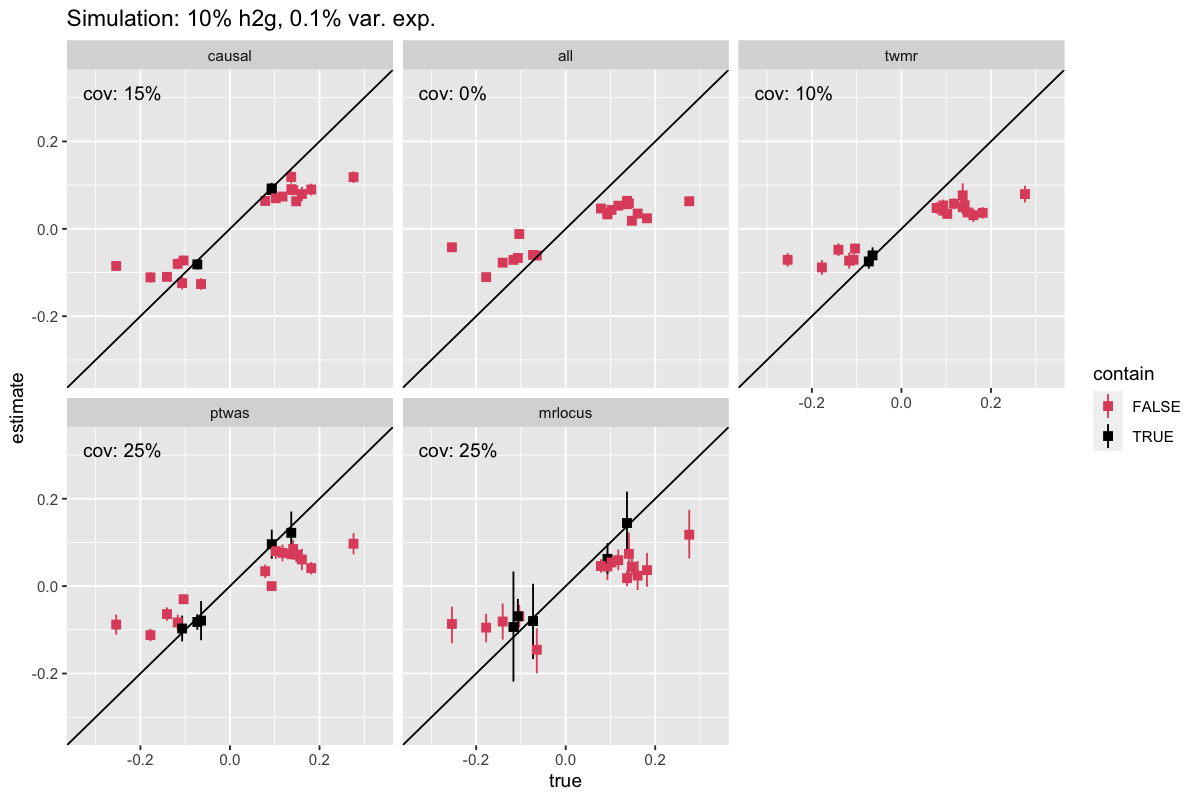
\includegraphics[width=.8\textwidth]{figs/cover5.png}
  \caption{Coverage of confidence or credible intervals for the
    gene-to-trait effect in simulation G.}
\end{figure}

\begin{figure}[!ht]
  \centering
  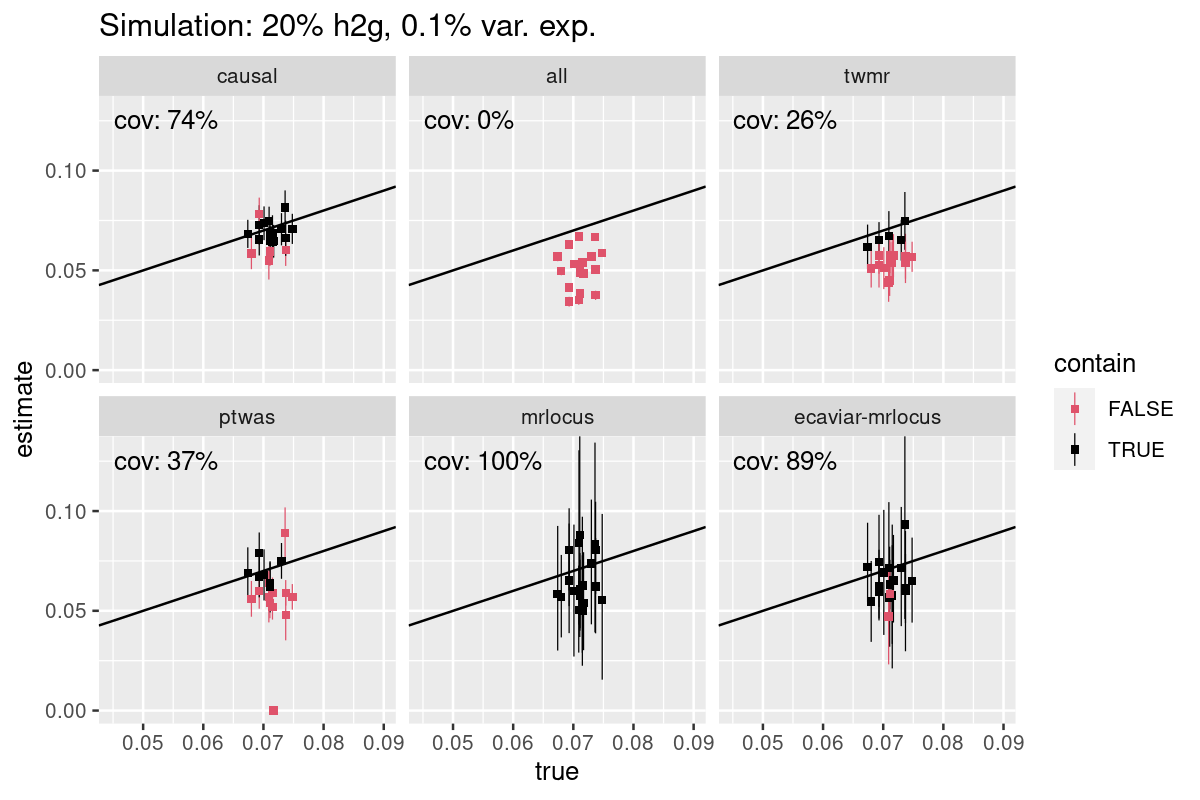
\includegraphics[width=.8\textwidth]{figs/cover7.png}
  \caption{Coverage of confidence or credible intervals for the
    gene-to-trait effect in simulation H.}
\end{figure}

\begin{figure}[!ht]
  \centering
  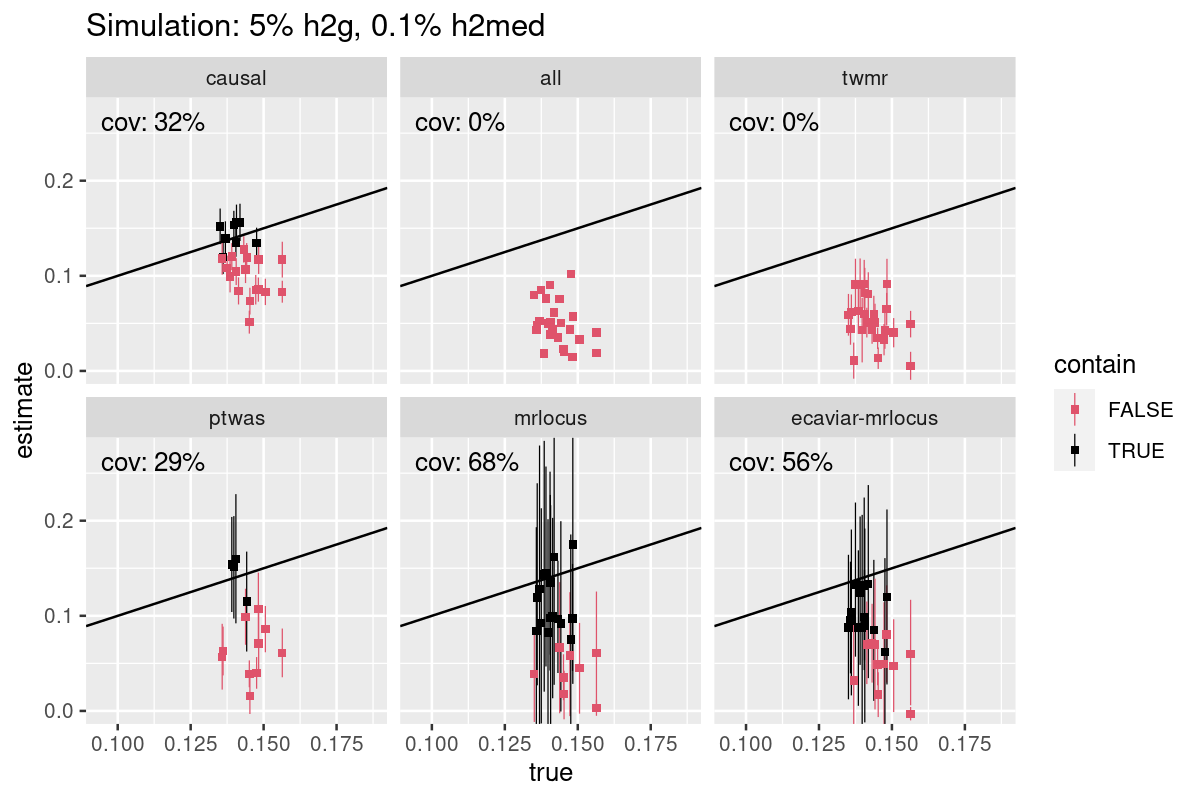
\includegraphics[width=.8\textwidth]{figs/cover9.png}
  \caption{Coverage of confidence or credible intervals for the
    gene-to-trait effect in simulation I.}
\end{figure}

\begin{figure}[!ht]
  \centering
  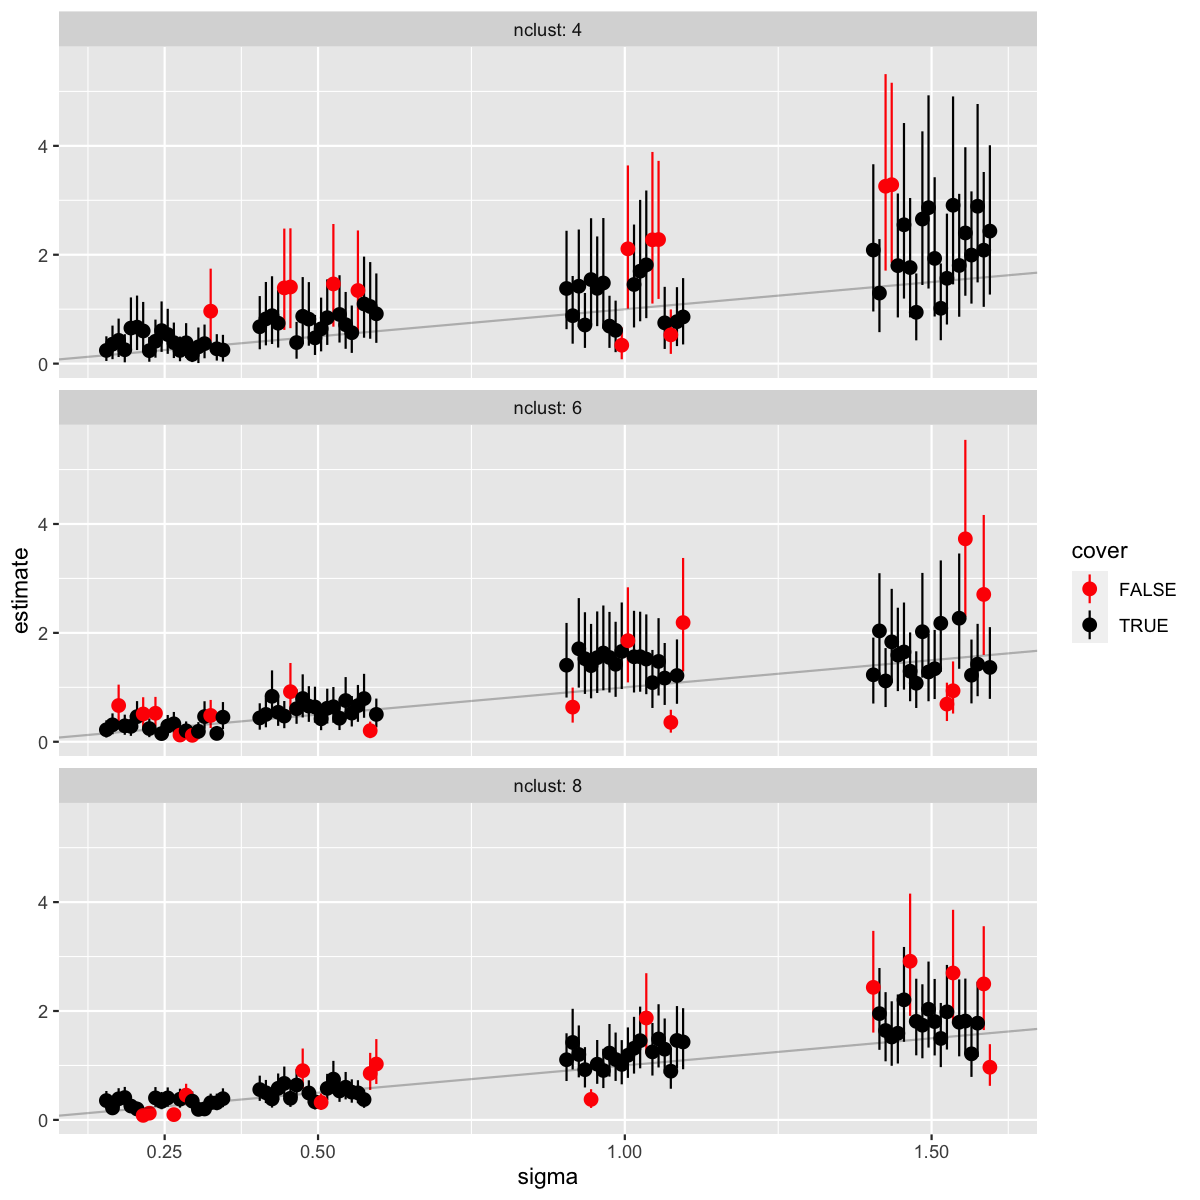
\includegraphics[width=.7\textwidth]{figs/sigma_est.png}
  \caption{Simulation assessing MRLocus' estimation of the scale of
    dispersion ($\sigma$) across independent signal clusters. The
    summary statistics for eQTL and GWAS were generated from a
    multivariate normal distribution as in the eCAVIAR model, using a
    simulated LD matrix. The true slope ($\alpha$) was set to 1, the
    true $\sigma$ varied among the values $\{0.25, 0.5, 1, 1.5\}$
    (x-axis), and the number of LD-independent clusters varied between
    4, 6, and 8 (top, middle, bottom panels), with 20 iterations
    per setting (plotted with horizontal spacing to avoid
    overplotting).  The posterior mean is indicated with a dot, while
    80\% quantile-based credible intervals and their coverage of the
    true value are indicated with the line and its color. The
    simulation script is included within the MRLocus package test
    directory, as an R script \texttt{"test\_sigma.R"}.}
\end{figure}

\begin{figure}[!ht]
  \centering
  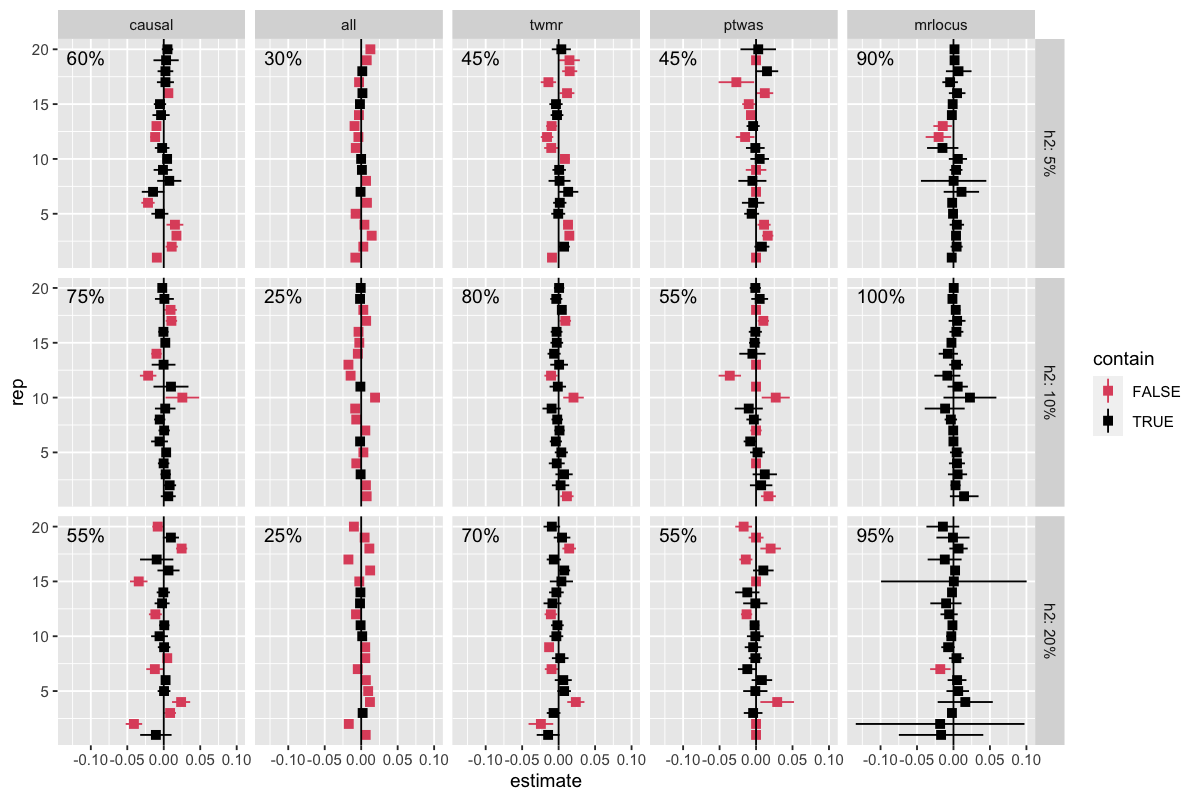
\includegraphics[width=\textwidth]{figs/nullplot.png}
  \caption{Coverage of confidence or credible intervals for the 3 null
    simulation settings.}
\end{figure}

\begin{figure}[!ht]
  \centering
  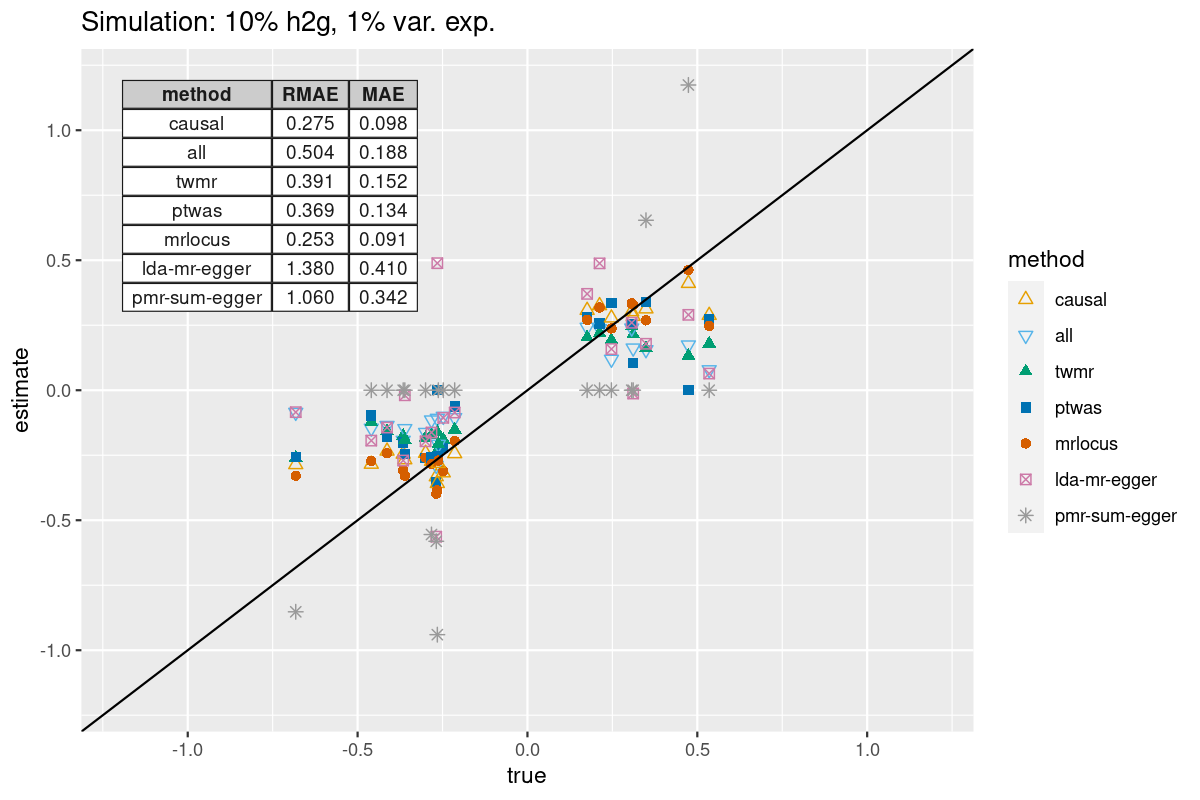
\includegraphics[width=.52\textwidth]{figs/sim1extra.png}
  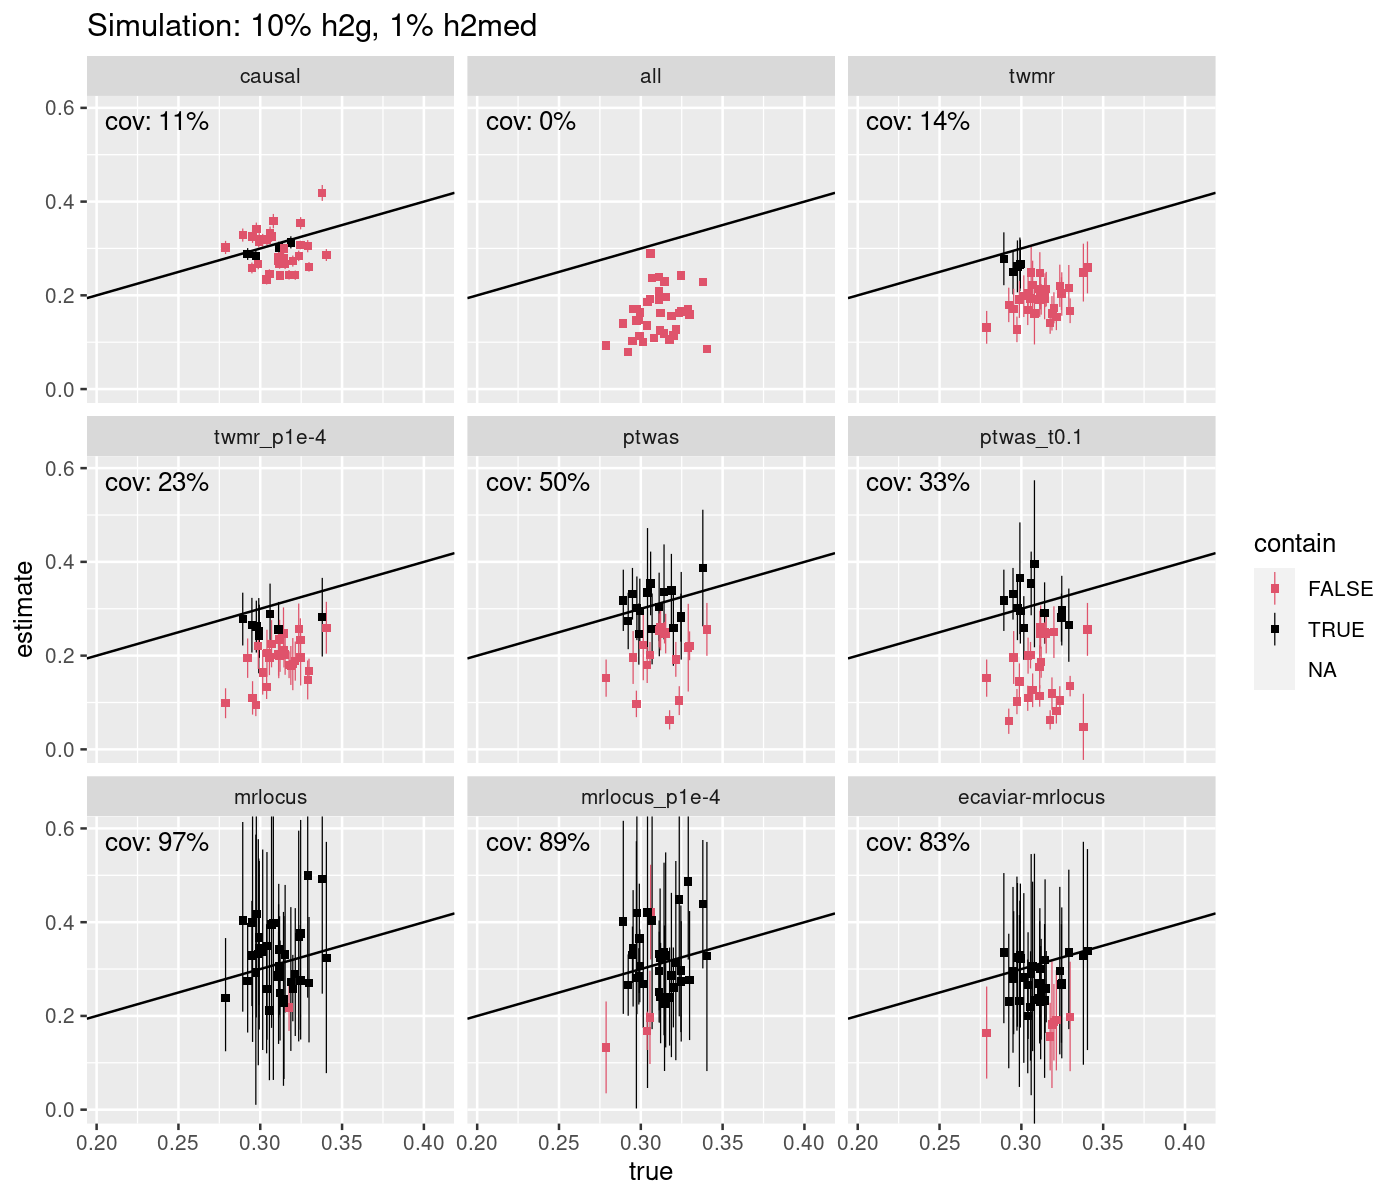
\includegraphics[width=.4\textwidth]{figs/cover1extra.png} \\
  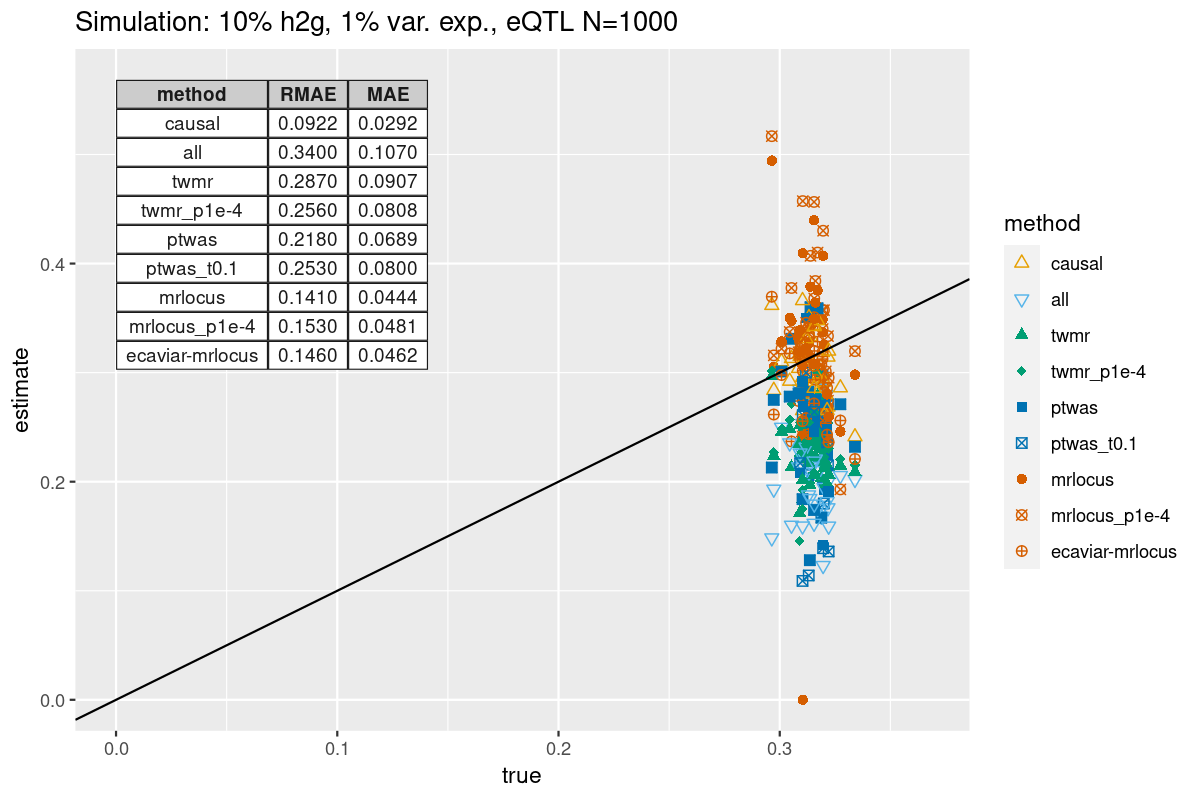
\includegraphics[width=.52\textwidth]{figs/simhigh_nextra.png}
  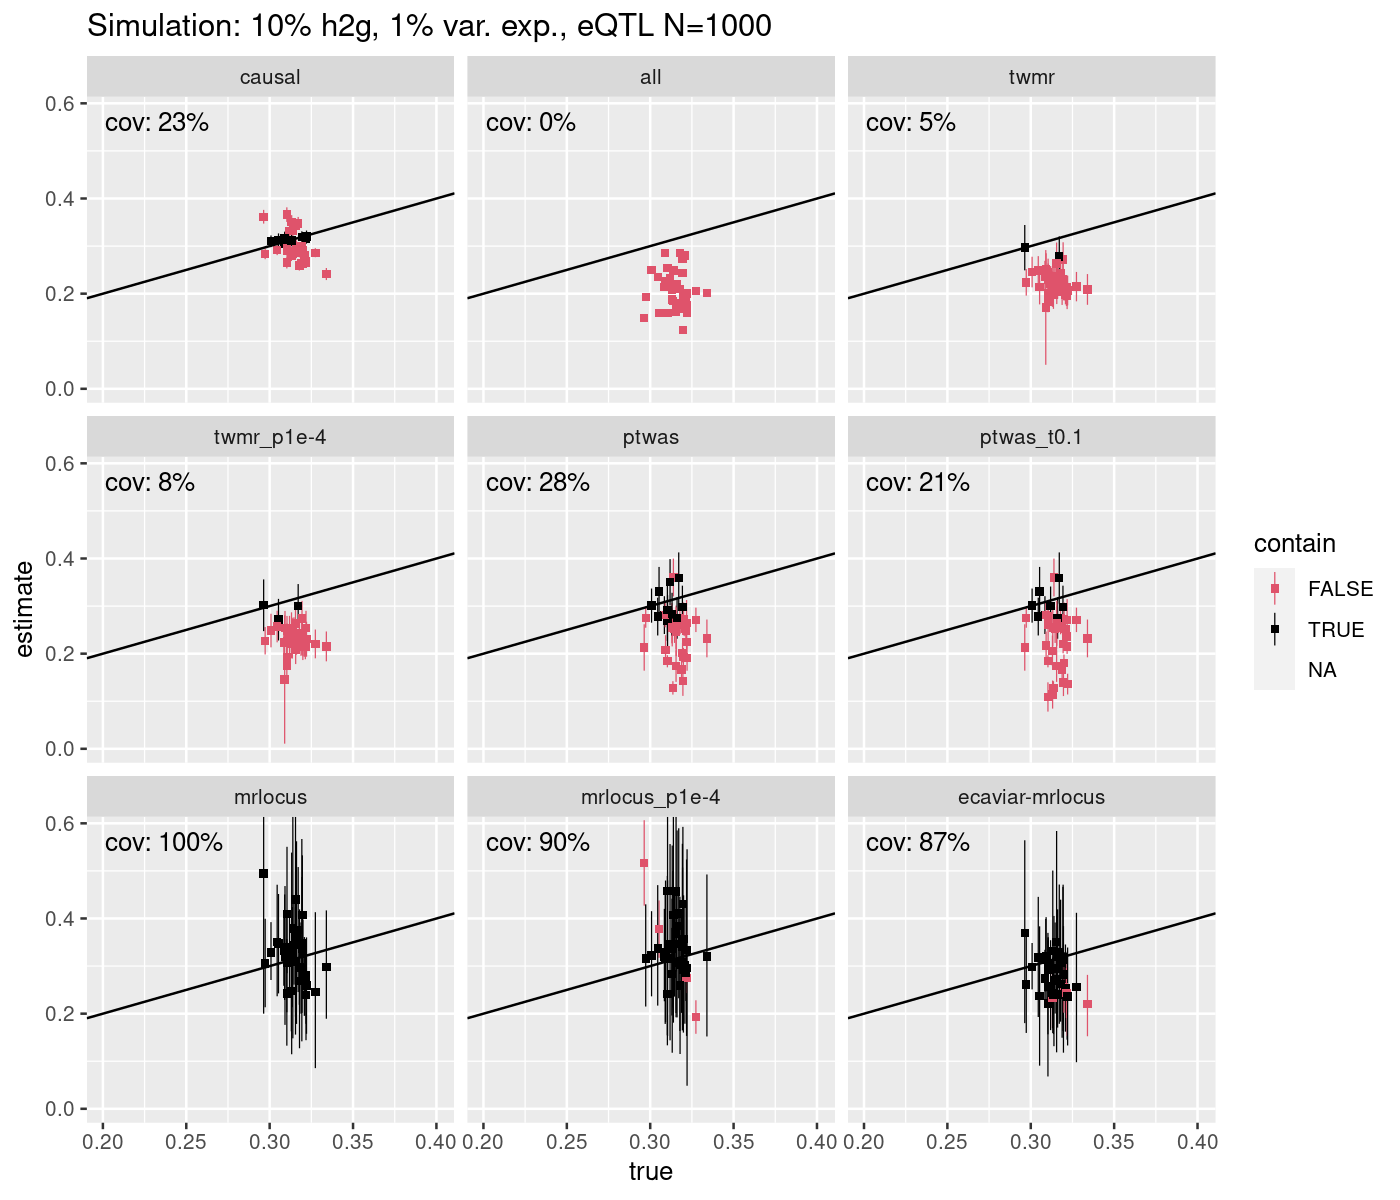
\includegraphics[width=.4\textwidth]{figs/coverhigh_nextra.png}
  \caption{Alternate thresholds...}
\end{figure}

\begin{figure}[!ht]
  \centering
  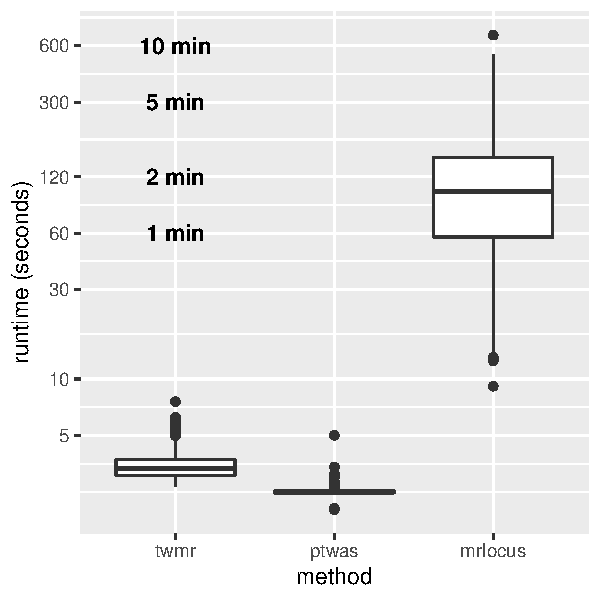
\includegraphics[width=.7\textwidth]{figs/runtime}
  \caption{Runtime for TWMR, PTWAS, and MRLocus on the 240
    simulations. The runtime for a single locus using a single core is
    shown on the y-axis (log scale).}
\end{figure}

%% \begin{figure}[!ht]
%%   \centering
%%   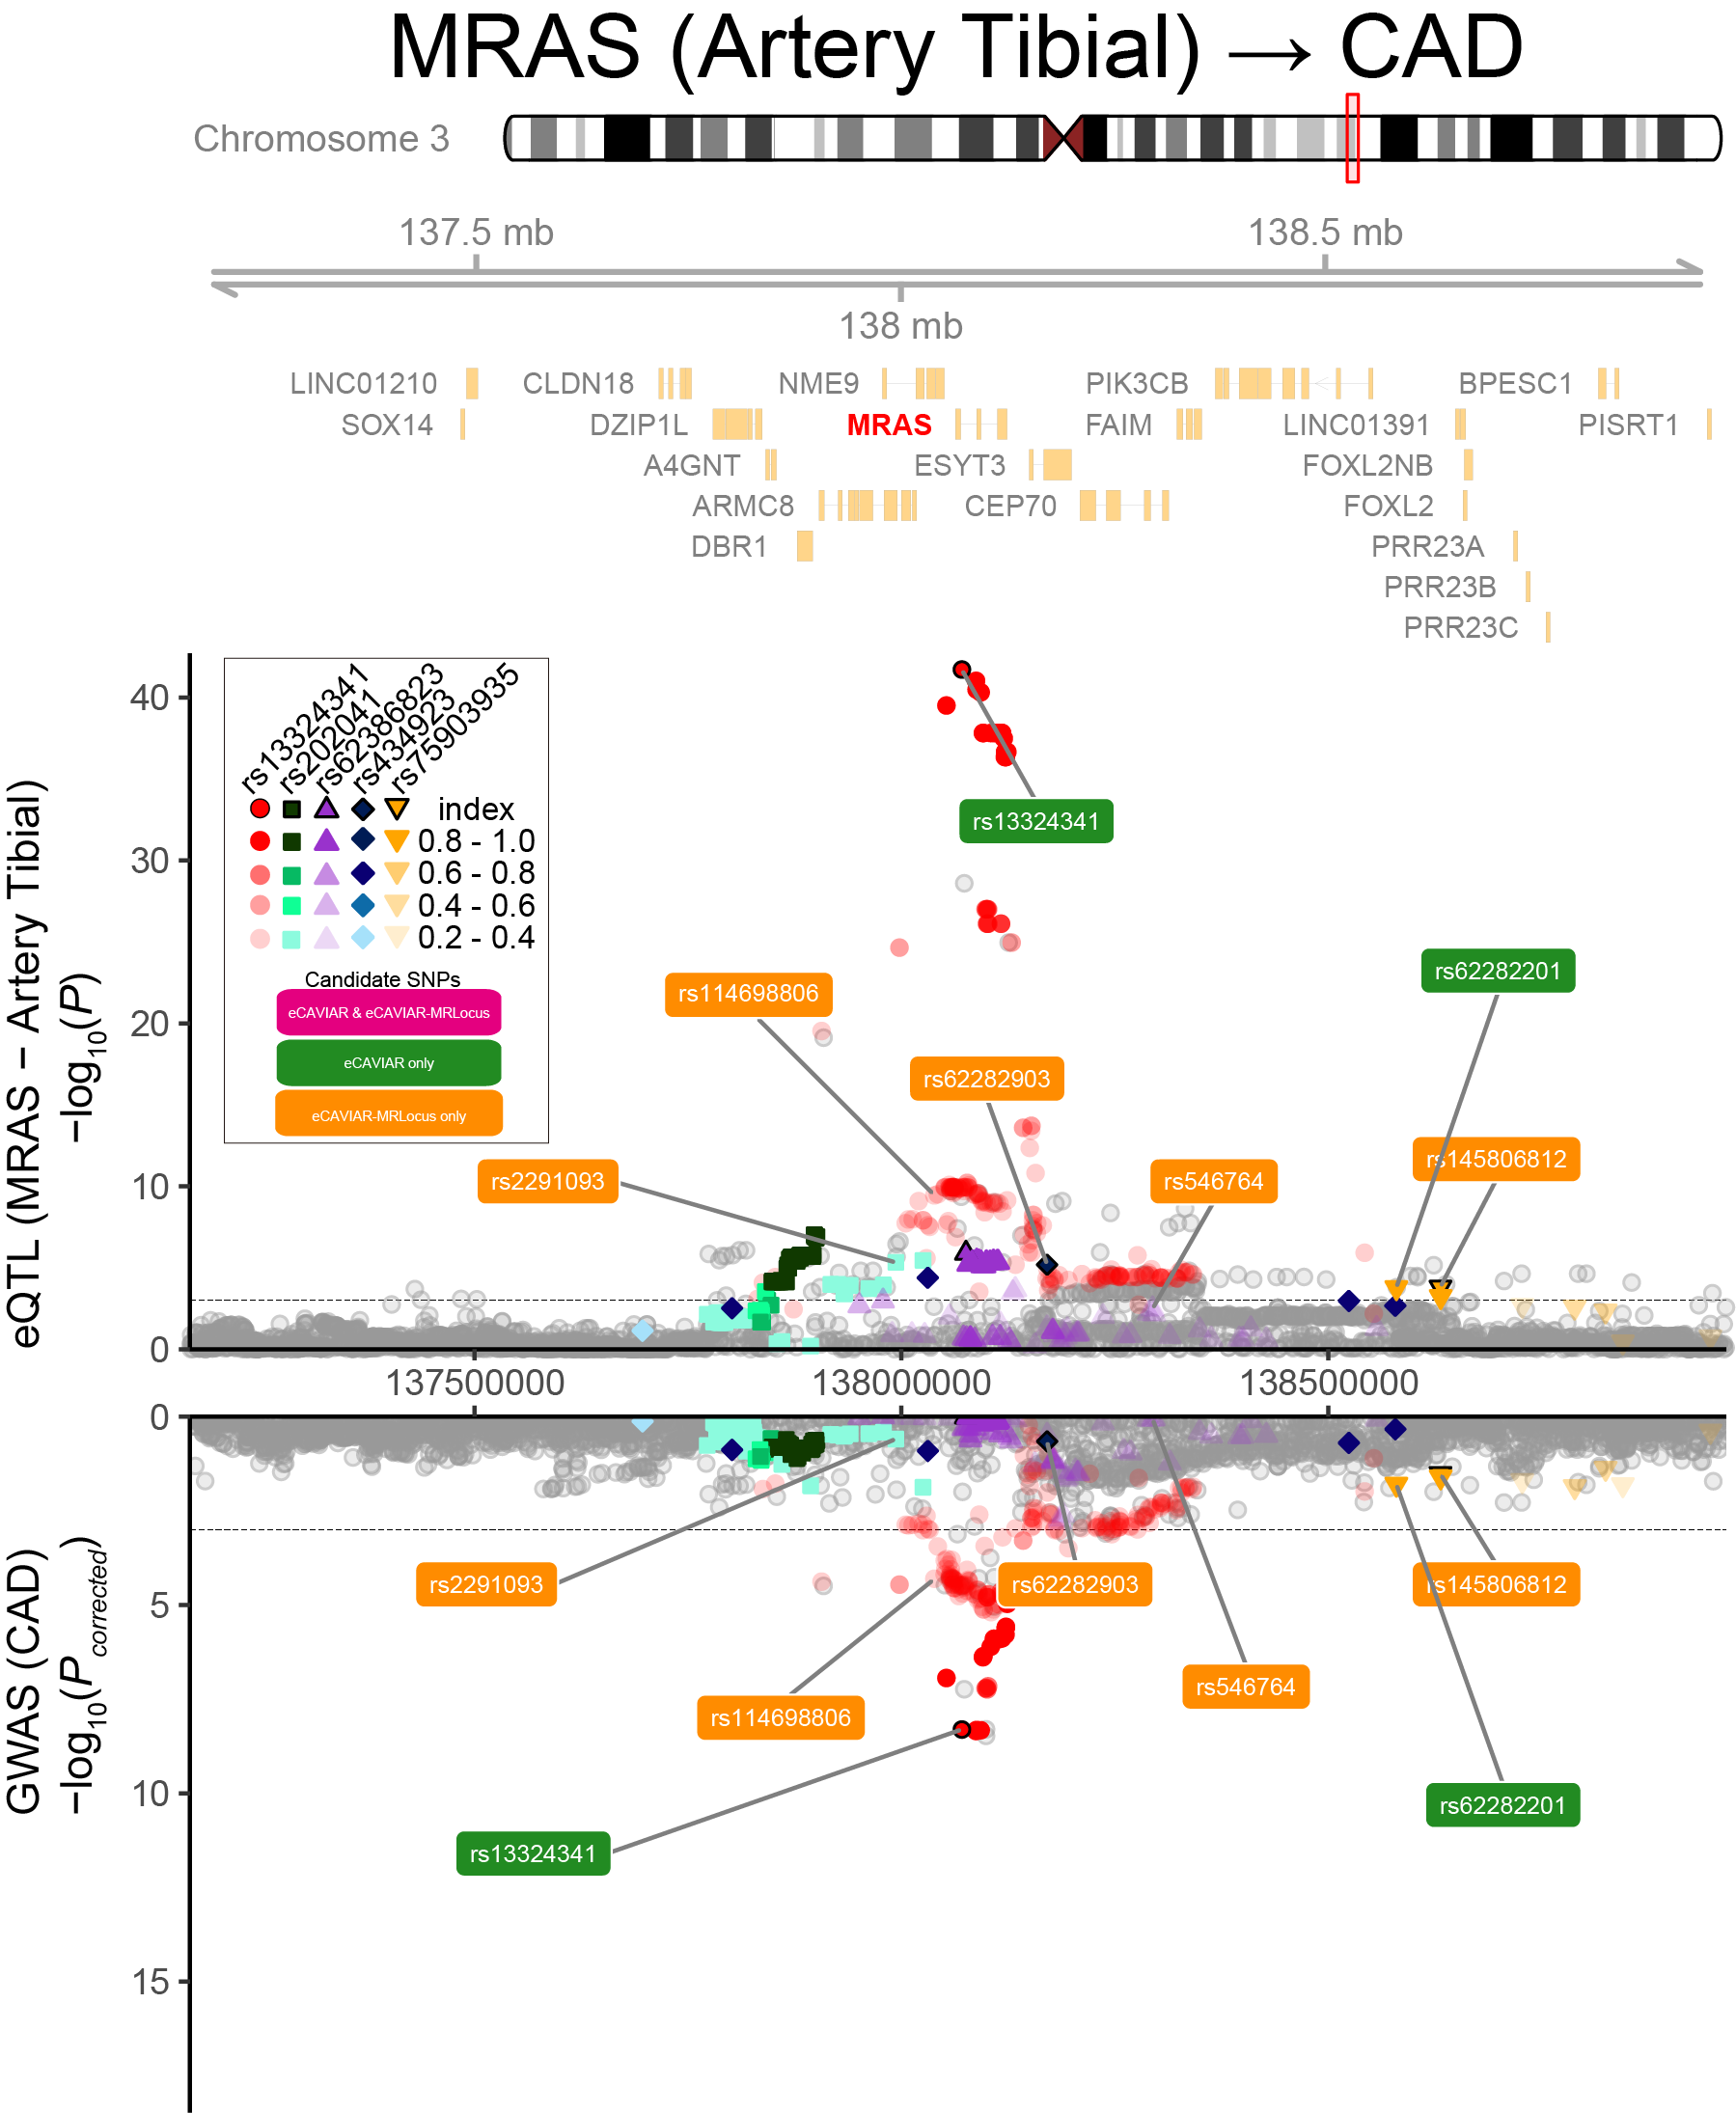
\includegraphics[width=.7\textwidth]{figs/region/regionplot.MRAS_Artery_Tibial_CAD.20201218.png}
%%   \caption{Colocalized signals in the \emph{MRAS} region. From top panel to
%%     bottom, gene model (NCBI Refseq), eQTL for MRAS in artery tibial
%%     (GTEx; N = 663) and CAD association within CARDIoGRAMplusC4D
%%     (\Ncase = 60,801 and \Ncontrol = 123,504) (M. Nikpay et al.,
%%     2015). LD was calculated to independent SNPs within 1KG EUR and
%%     colored accordingly. Symbols indicate independent co-localized
%%     ($r^2 > 0.4$) eQTL-GWAS pairs. Dashed line indicates a significance
%%     threshold at p = 0.001 or p = 5x$10^{-8}$ for eQTL and GWAS
%%     respectively.}
%% \end{figure}

%% \begin{figure}[!ht]
%%   \centering
%%   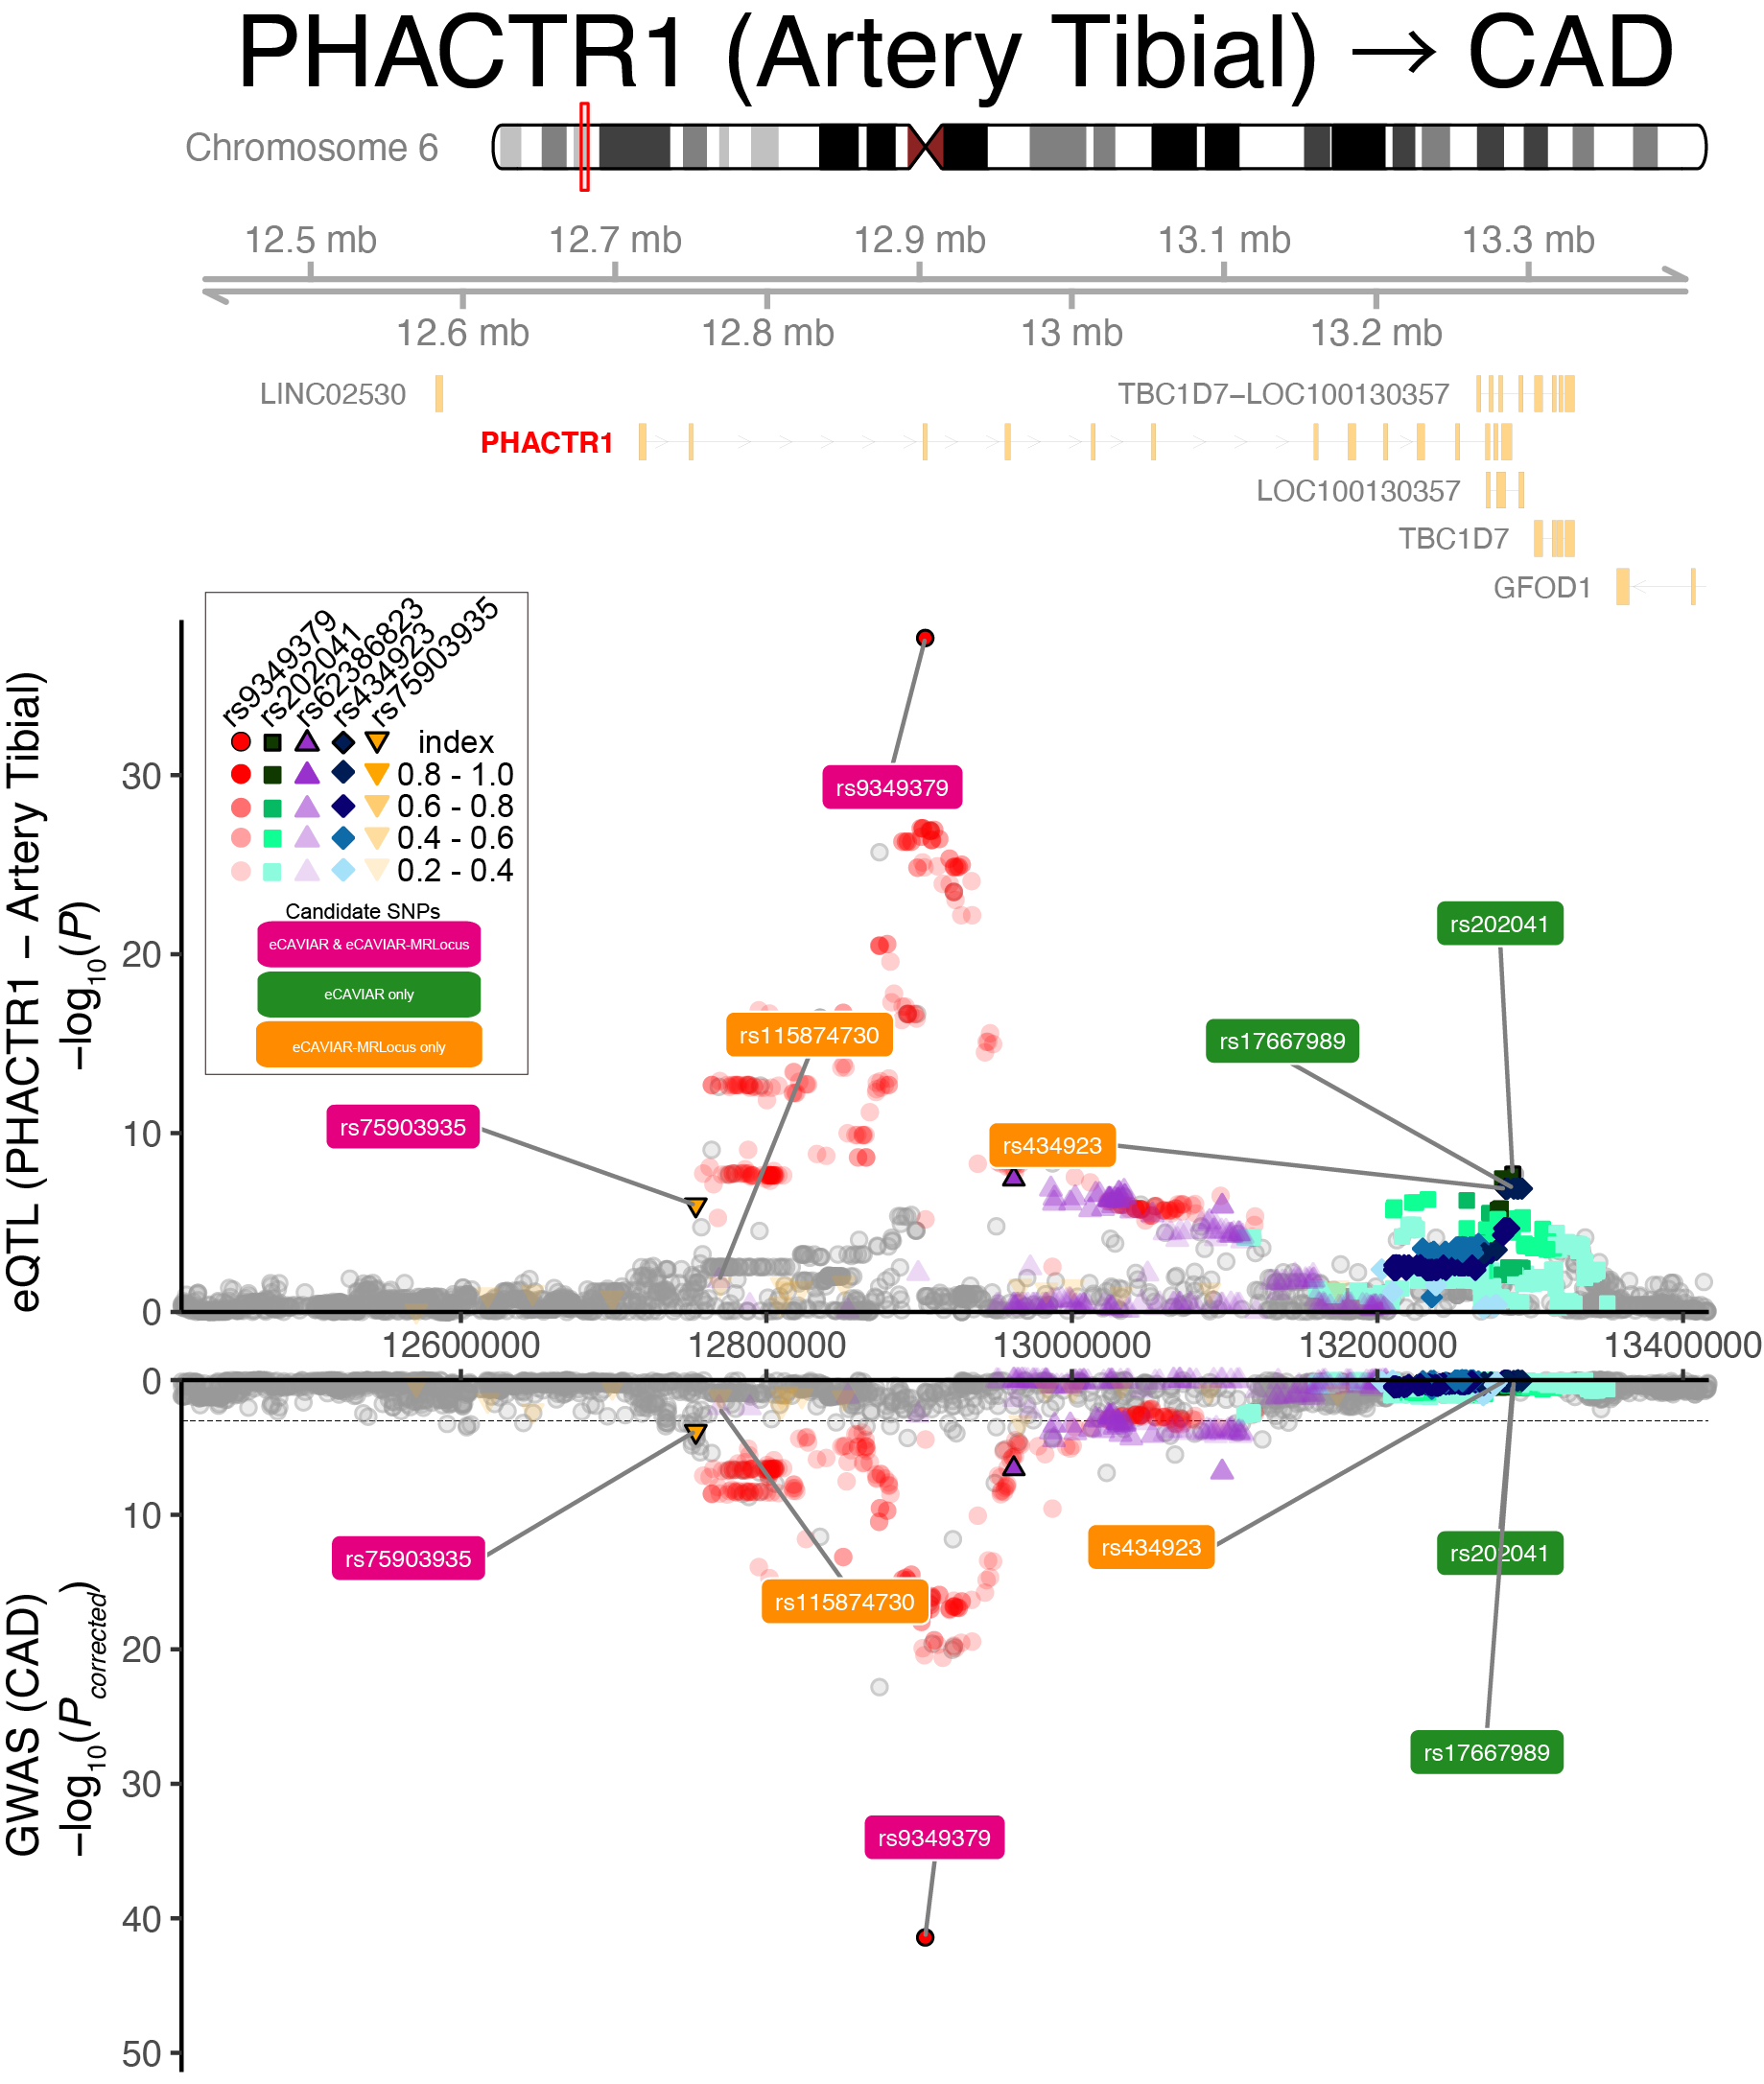
\includegraphics[width=.7\textwidth]{figs/region/regionplot.PHACTR1_Artery_Tibial_CAD.20201218.edit.png}
%%   \caption{Colocalized signals in the \emph{PHACTR1} region. From top
%%     panel to bottom, gene model (NCBI Refseq), eQTL for PHACTR1 in
%%     artery tibial (GTEx; N = 663) and CAD association within
%%     CARDIoGRAMplusC4D (\Ncase = 60,801 and \Ncontrol = 123,504)
%%     (M. Nikpay et al., 2015). LD was calculated to independent SNPs
%%     within 1KG EUR and colored accordingly. Symbols indicate
%%     independent co-localized ($r^2 > 0.4$) eQTL-GWAS pairs. Dashed
%%     line indicates a significance threshold at p = 0.001 or p =
%%     5x$10^{-8}$ for eQTL and GWAS respectively.} 
%% \end{figure}

%% \begin{figure}[!ht]
%%   \centering
%%   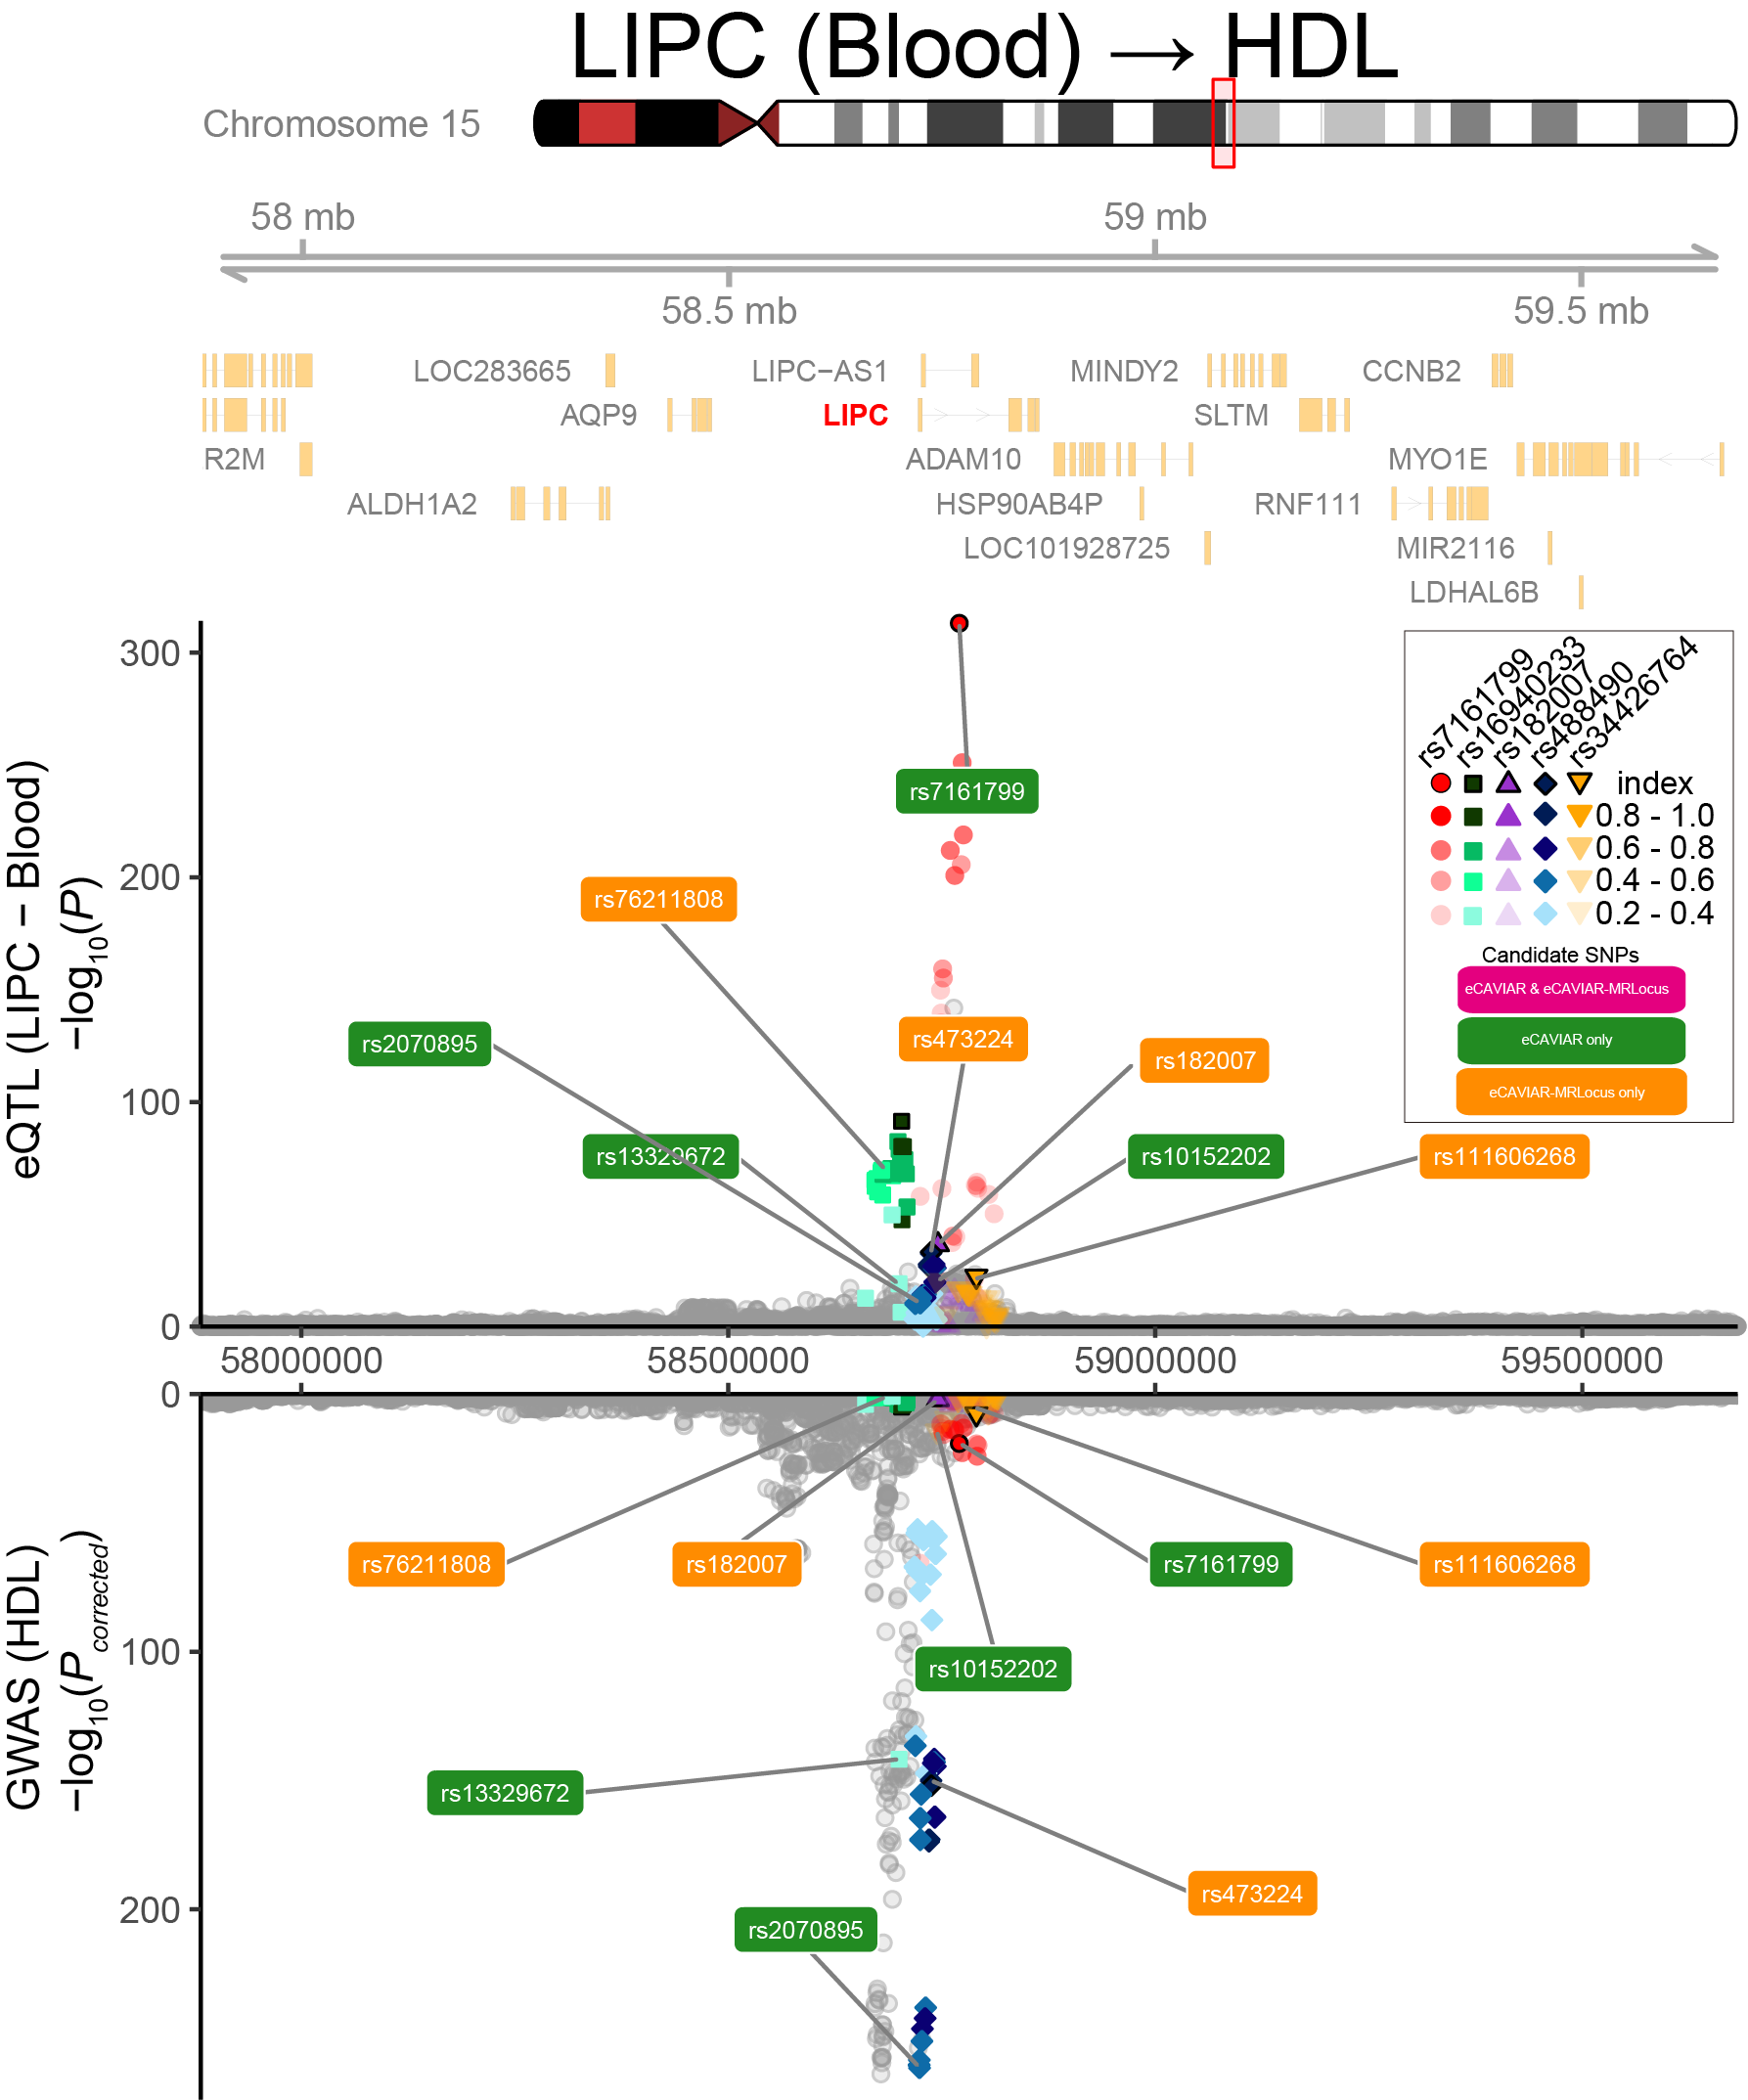
\includegraphics[width=.7\textwidth]{figs/region/regionplot.LIPC_Blood_HDL_UKBB.20201218.edit.png}
%%   \caption{Colocalized signals in the \emph{LIPC} region for blood
%%     eQTL.}
%% \end{figure}  

%% \begin{figure}[!ht]
%%   \centering
%%   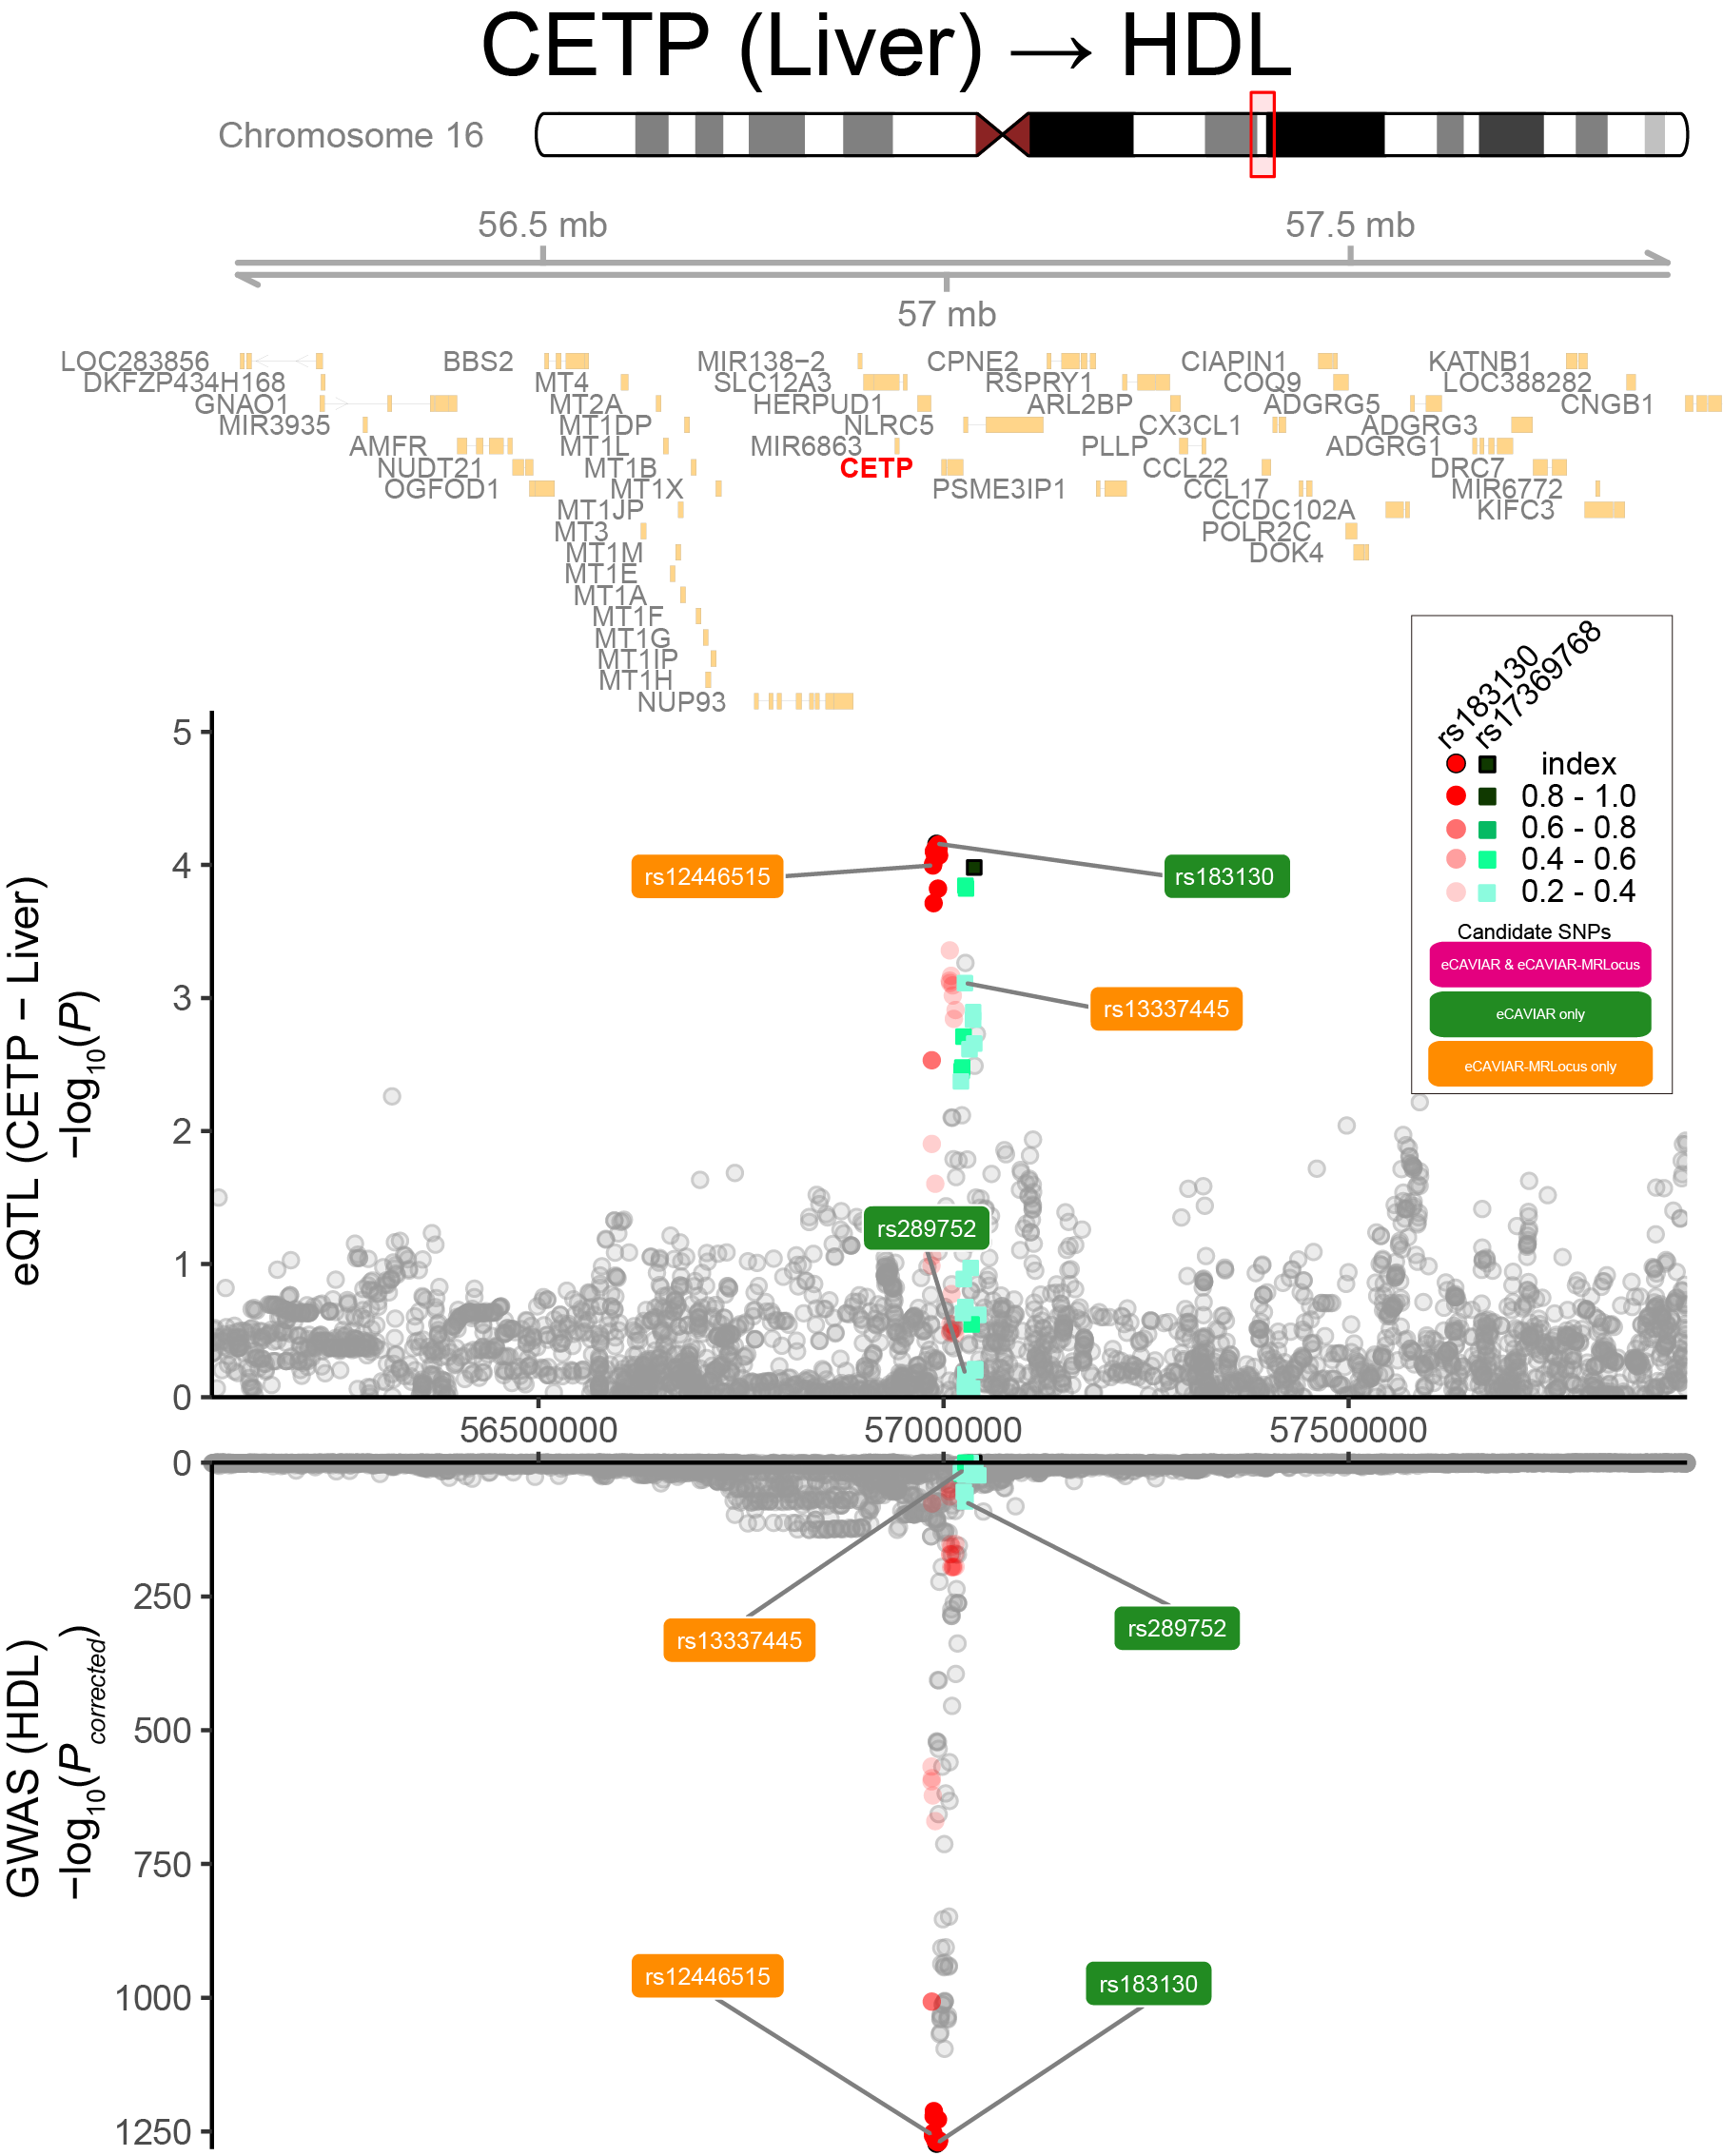
\includegraphics[width=.7\textwidth]{figs/region/regionplot.CETP_Liver_HDL_UKBB.20201218.edit.png}
%%   \caption{Colocalized signals in the \emph{CETP} region. From top
%%     panel to bottom, gene model (NCBI Refseq), eQTL for CETP in liver
%%     (N = 588) (Strunz et al., 2018) and HDL association within UKBB (N
%%     = 315,133). LD was calculated to independent SNPs within 1KG EUR
%%     and colored accordingly. Symbols indicate independent co-localized
%%     ($r^2 > 0.4$) eQTL-GWAS pairs. Dashed line indicates a significance
%%     threshold at p = 0.001 or p = 5x$10^{-8}$ for eQTL and GWAS
%%     respectively.} 
%% \end{figure}

%% \begin{figure}[!ht]
%%   \centering
%%   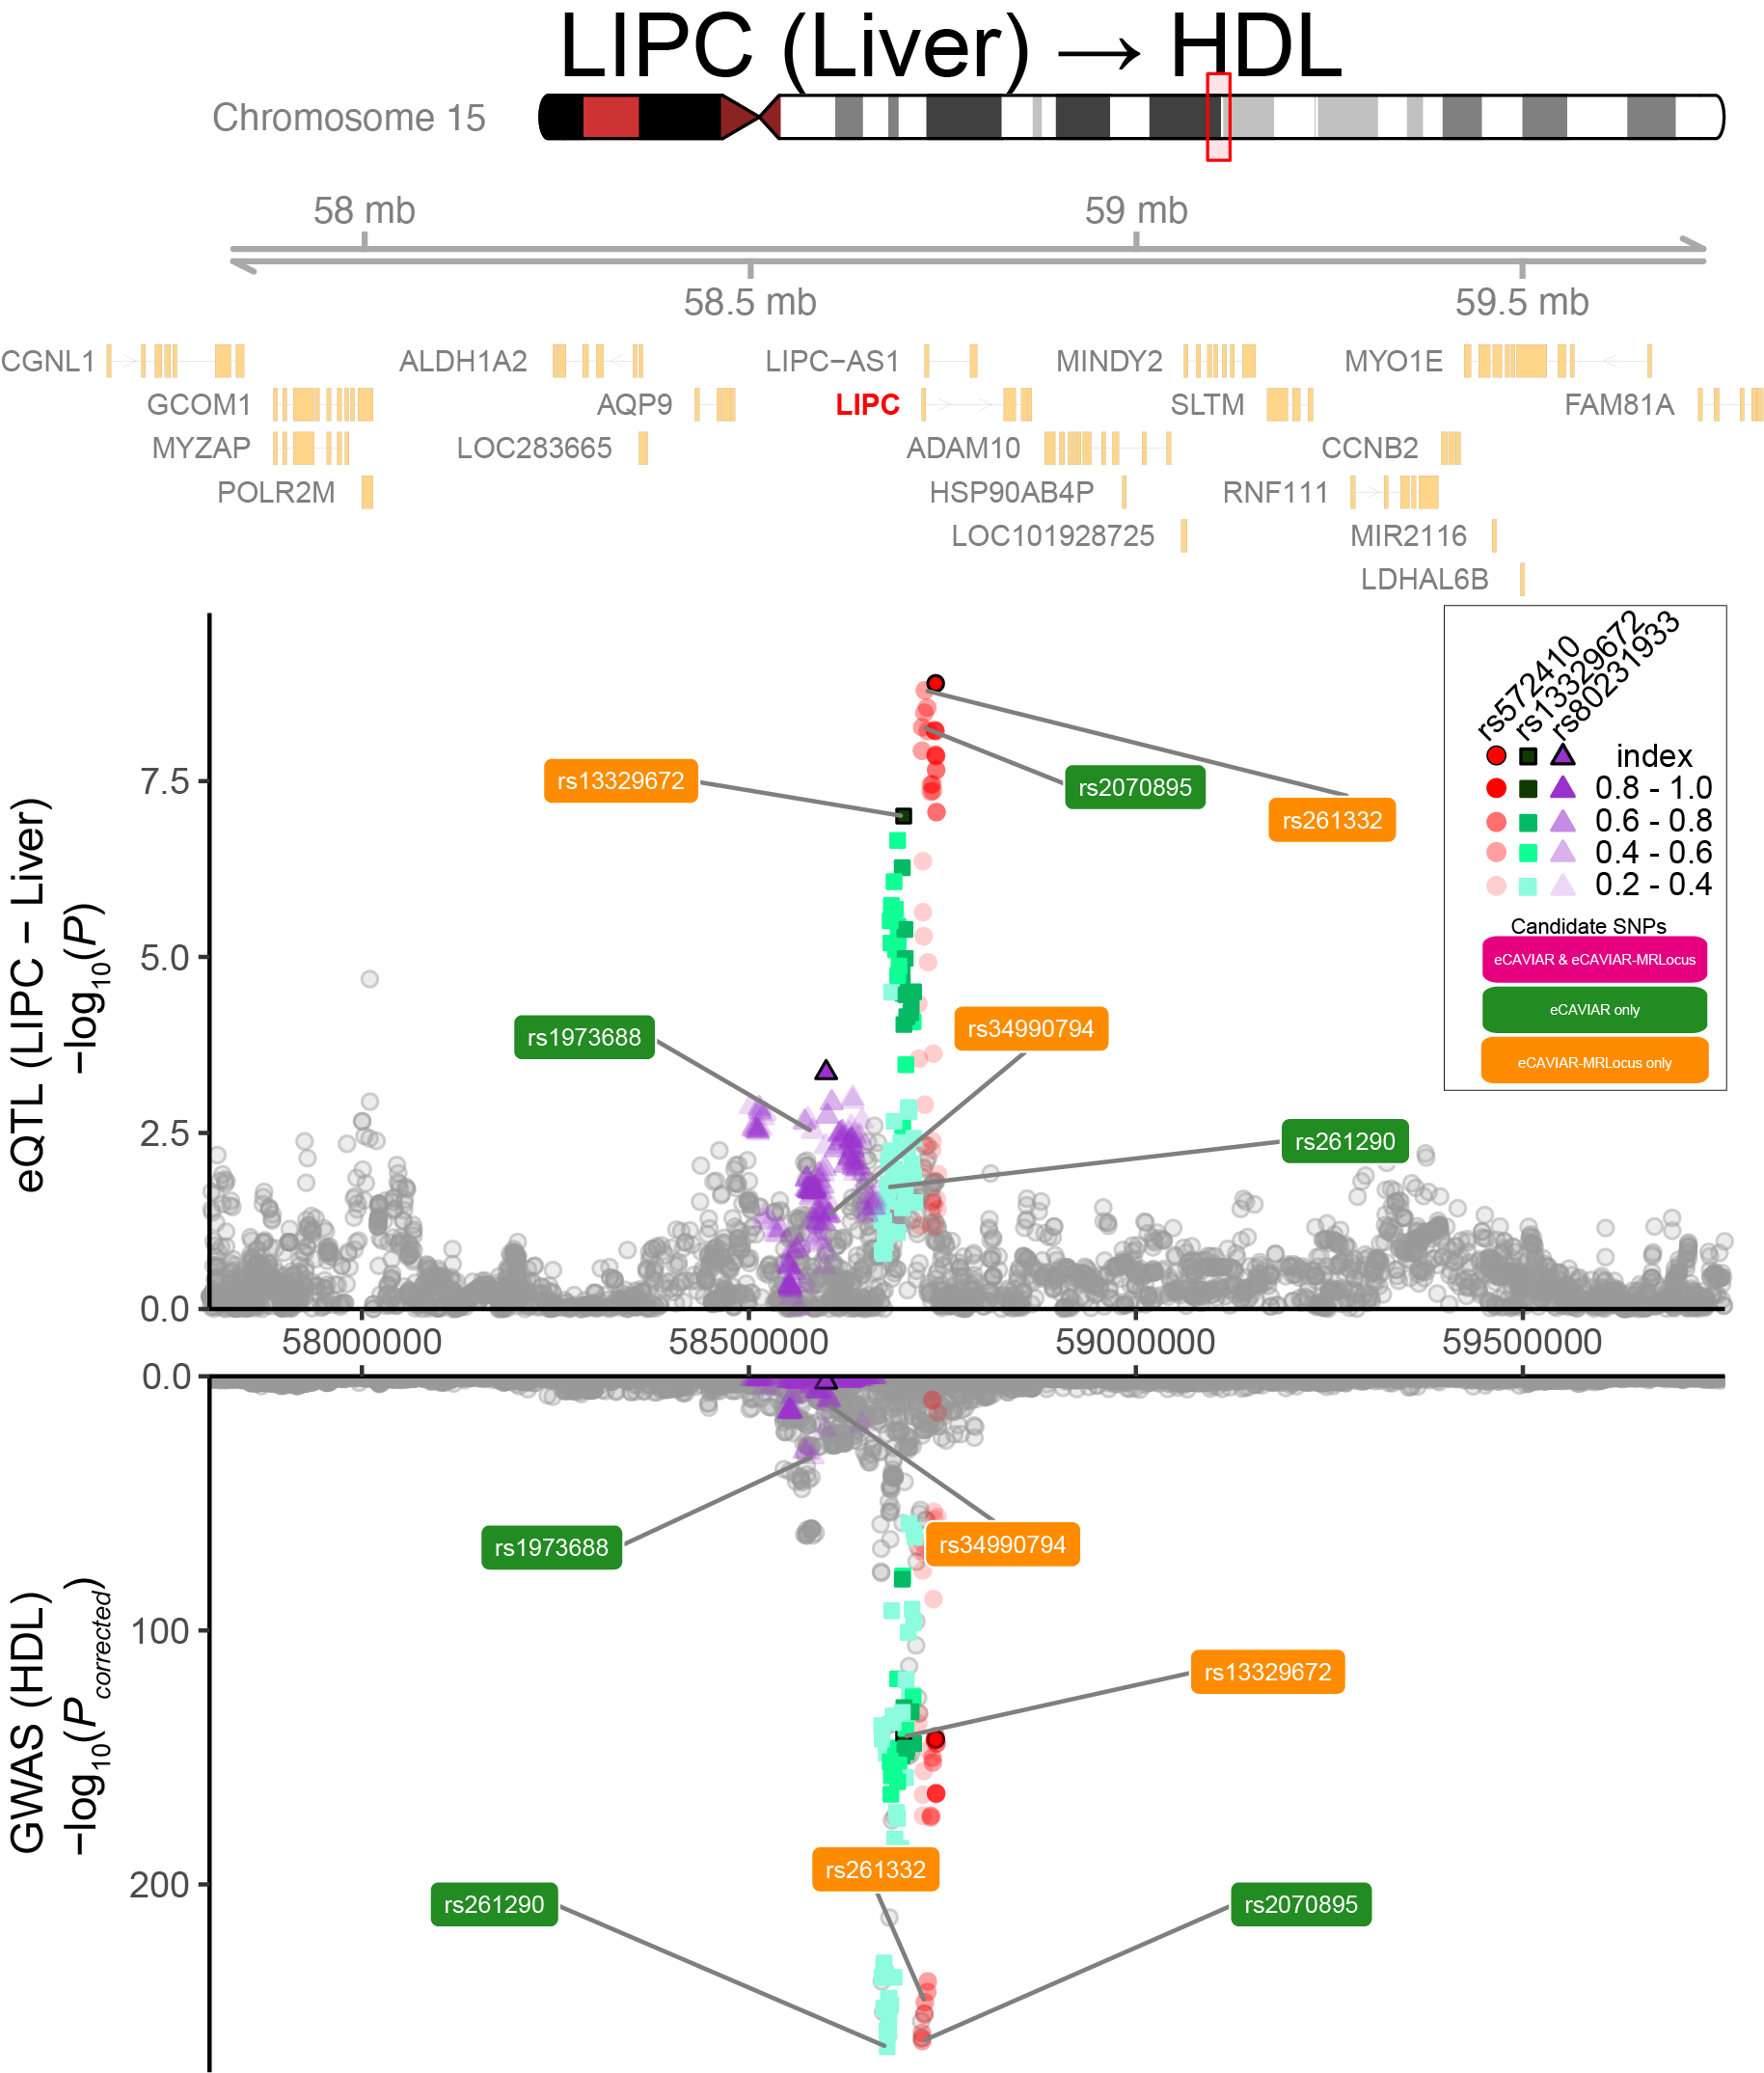
\includegraphics[width=.7\textwidth]{figs/region/regionplot.LIPC_Liver_HDL_UKBB.20201218.edit.png}
%%   \caption{Colocalized signals in the \emph{LIPC} region for liver eQTL. From top
%%     panel to bottom, gene model (NCBI Refseq), eQTL for LIPC in liver
%%     (N = 588) (Strunz et al., 2018) and HDL association within UKBB (N
%%     = 315,133). LD was calculated to independent SNPs within 1KG EUR
%%     and colored accordingly. Symbols indicate independent co-localized
%%     ($r^2> 0.4$) eQTL-GWAS pairs. Dashed line indicates a significance
%%     threshold at p = 0.001 or p = 5x$10^{-8}$ for eQTL and GWAS
%%     respectively.} 
%% \end{figure}

%% \begin{figure}[!ht]
%%   \centering
%%   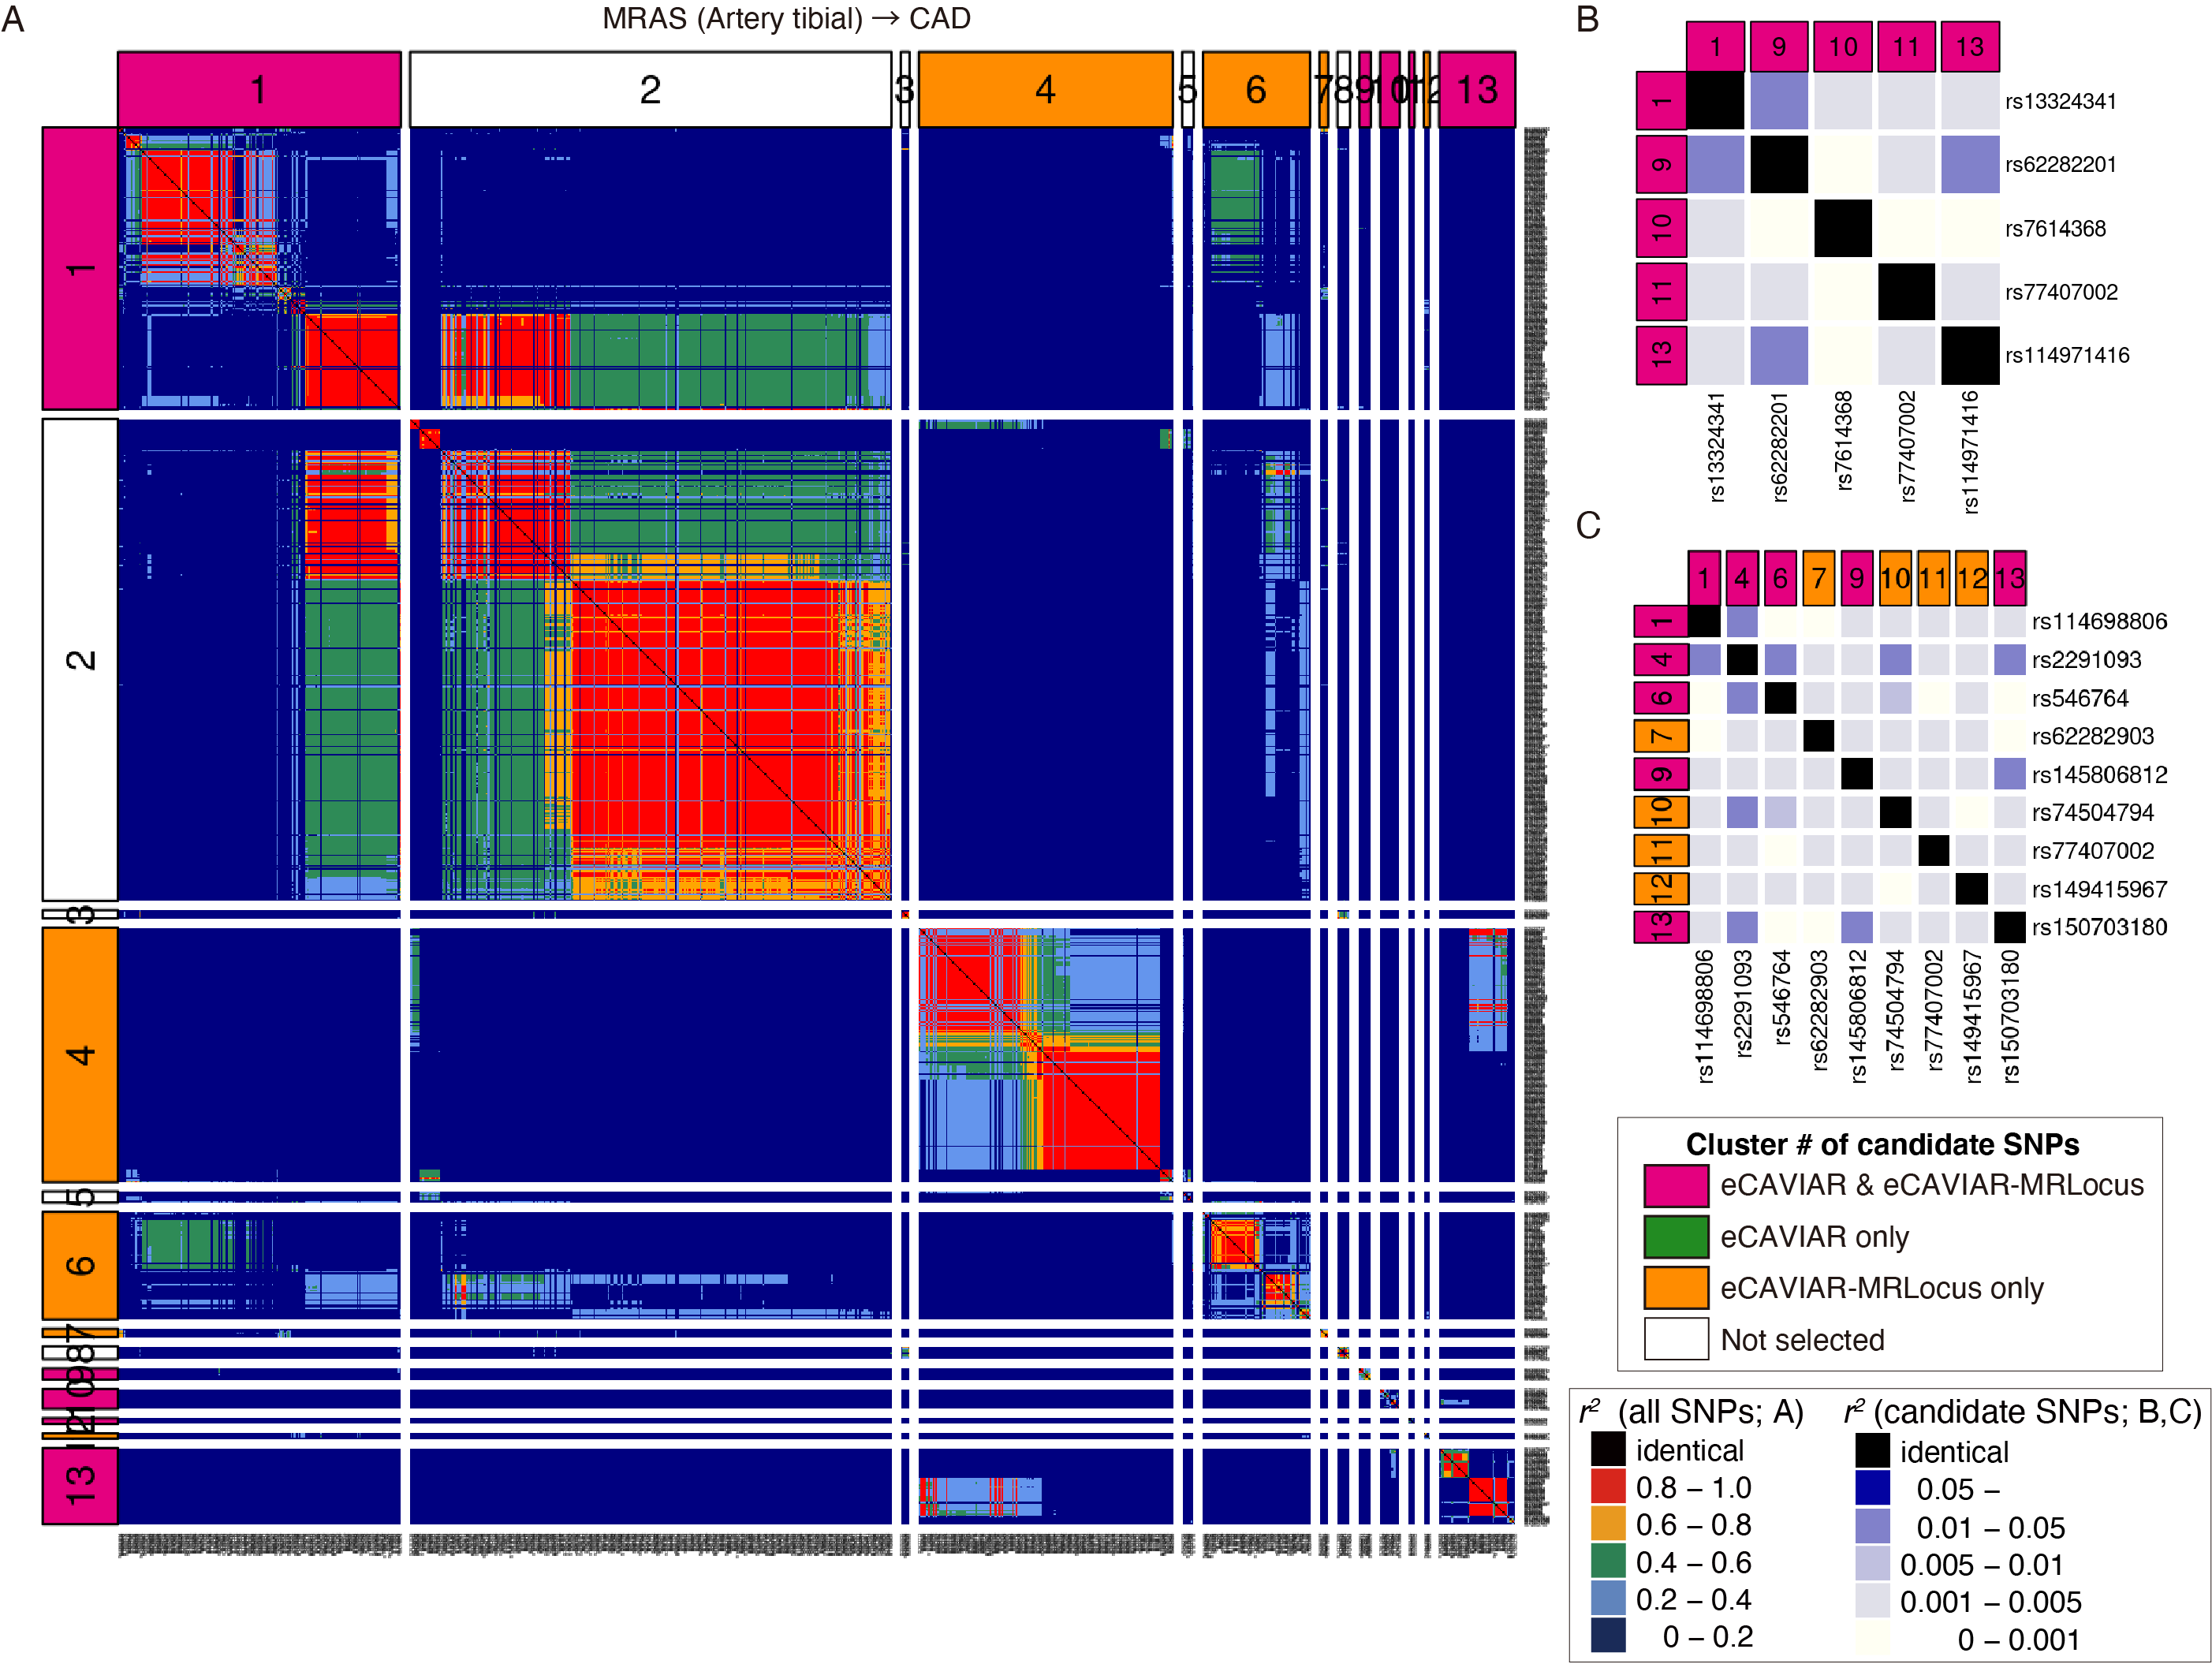
\includegraphics[width=.7\textwidth]{figs/region/heatmap_eQTLbase.Artery_MRAS_CAD.20201217.png}
%%   \caption{LD pattern across independent clusters from \emph{MRAS}
%%     eQTL (Artery tibial) and CAD GWAS. LD ($r^2$) between SNPs in
%%     independent clumps from \emph{MRAS} in artery tibial (columns) and
%%     CAD GWAS SNPs (rows). Color bars at the top and left represent
%%     cluster (pair) ID which is sorted by base position of index eQTL
%%     SNPs. LD was calculated to independent SNPs within 1KG EUR and
%%     colored accordingly.}
%%   \label{fig:ld1}
%% \end{figure}

%% \begin{figure}[!ht]
%%   \centering
%%   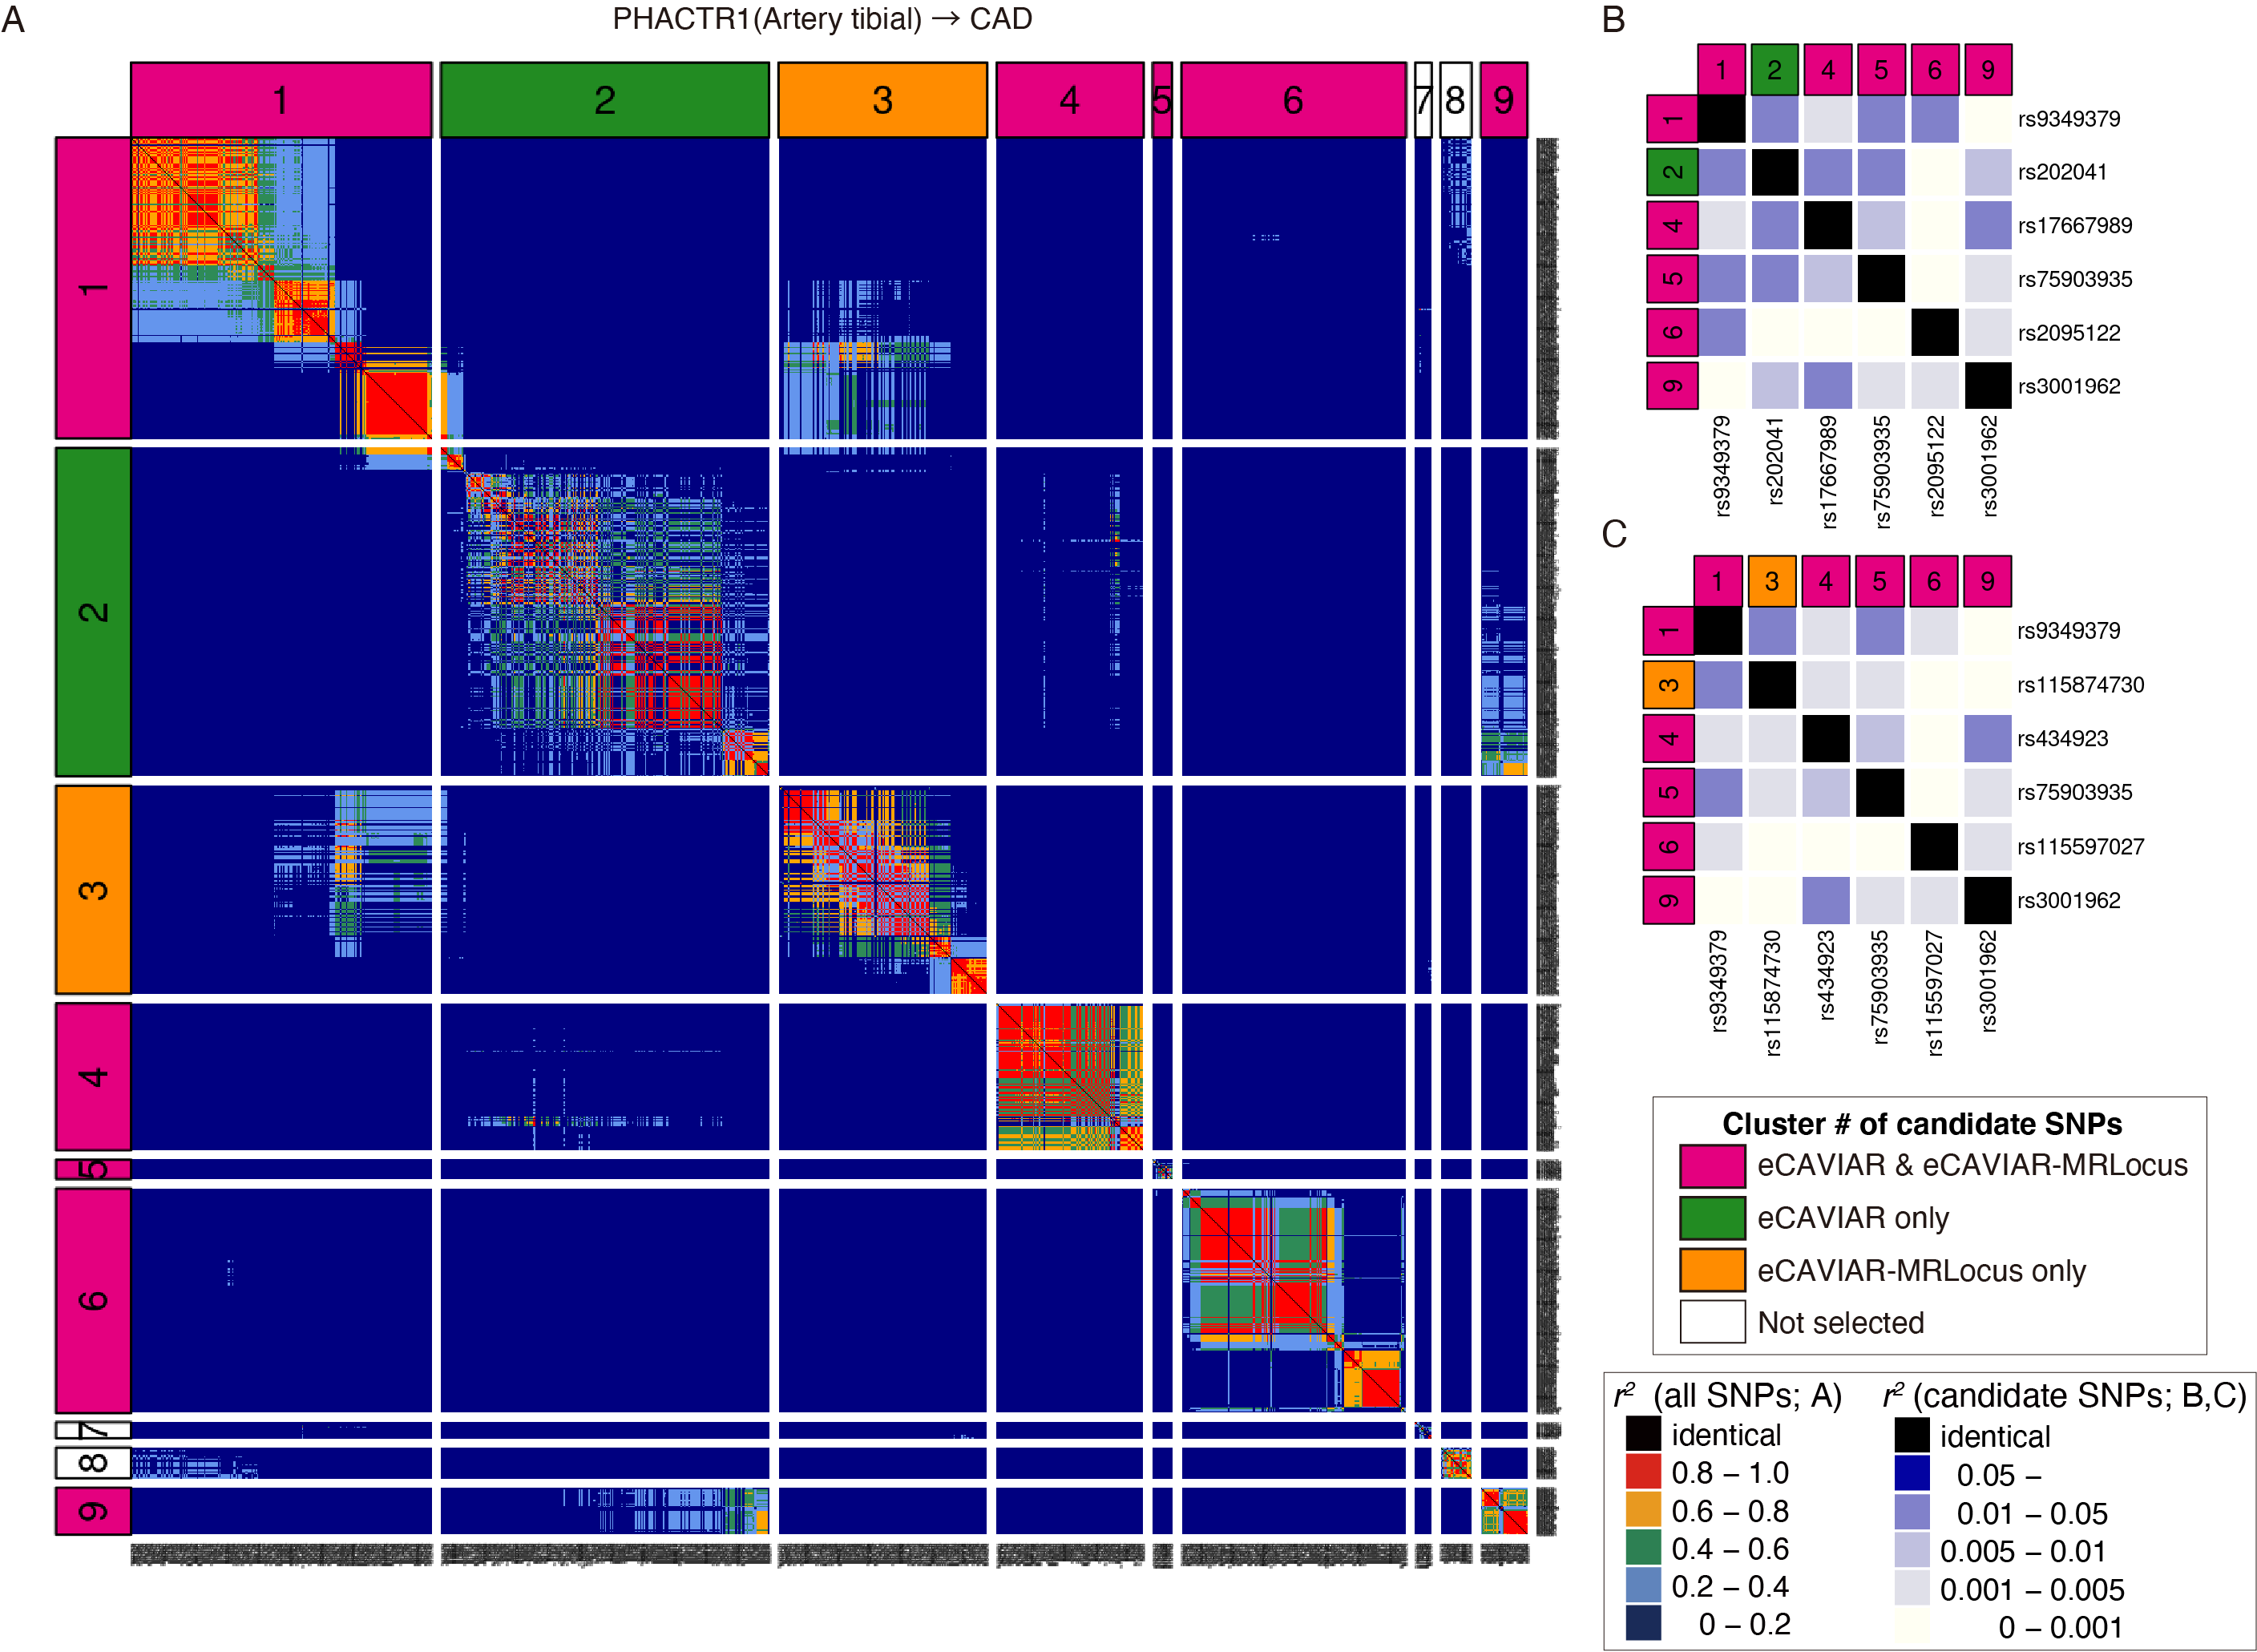
\includegraphics[width=.7\textwidth]{figs/region/heatmap_eQTLbase.Artery_PHACTR1_CAD.20201217.png}
%%   \caption{LD pattern across independent clusters from \emph{PHACTR1}
%%     eQTL (Artery tibial) and CAD GWAS. LD ($r^2$) between SNPs in
%%     independent clumps from \emph{PHACTR1} in artery tibial (columns)
%%     and CAD GWAS SNPs (rows). Color bars at the top and left represent
%%     cluster (pair) ID which is sorted by base position of index eQTL
%%     SNPs. LD was calculated to independent SNPs within 1KG EUR and
%%     colored accordingly.} 
%% \end{figure}

%% \begin{figure}[!ht]
%%   \centering
%%   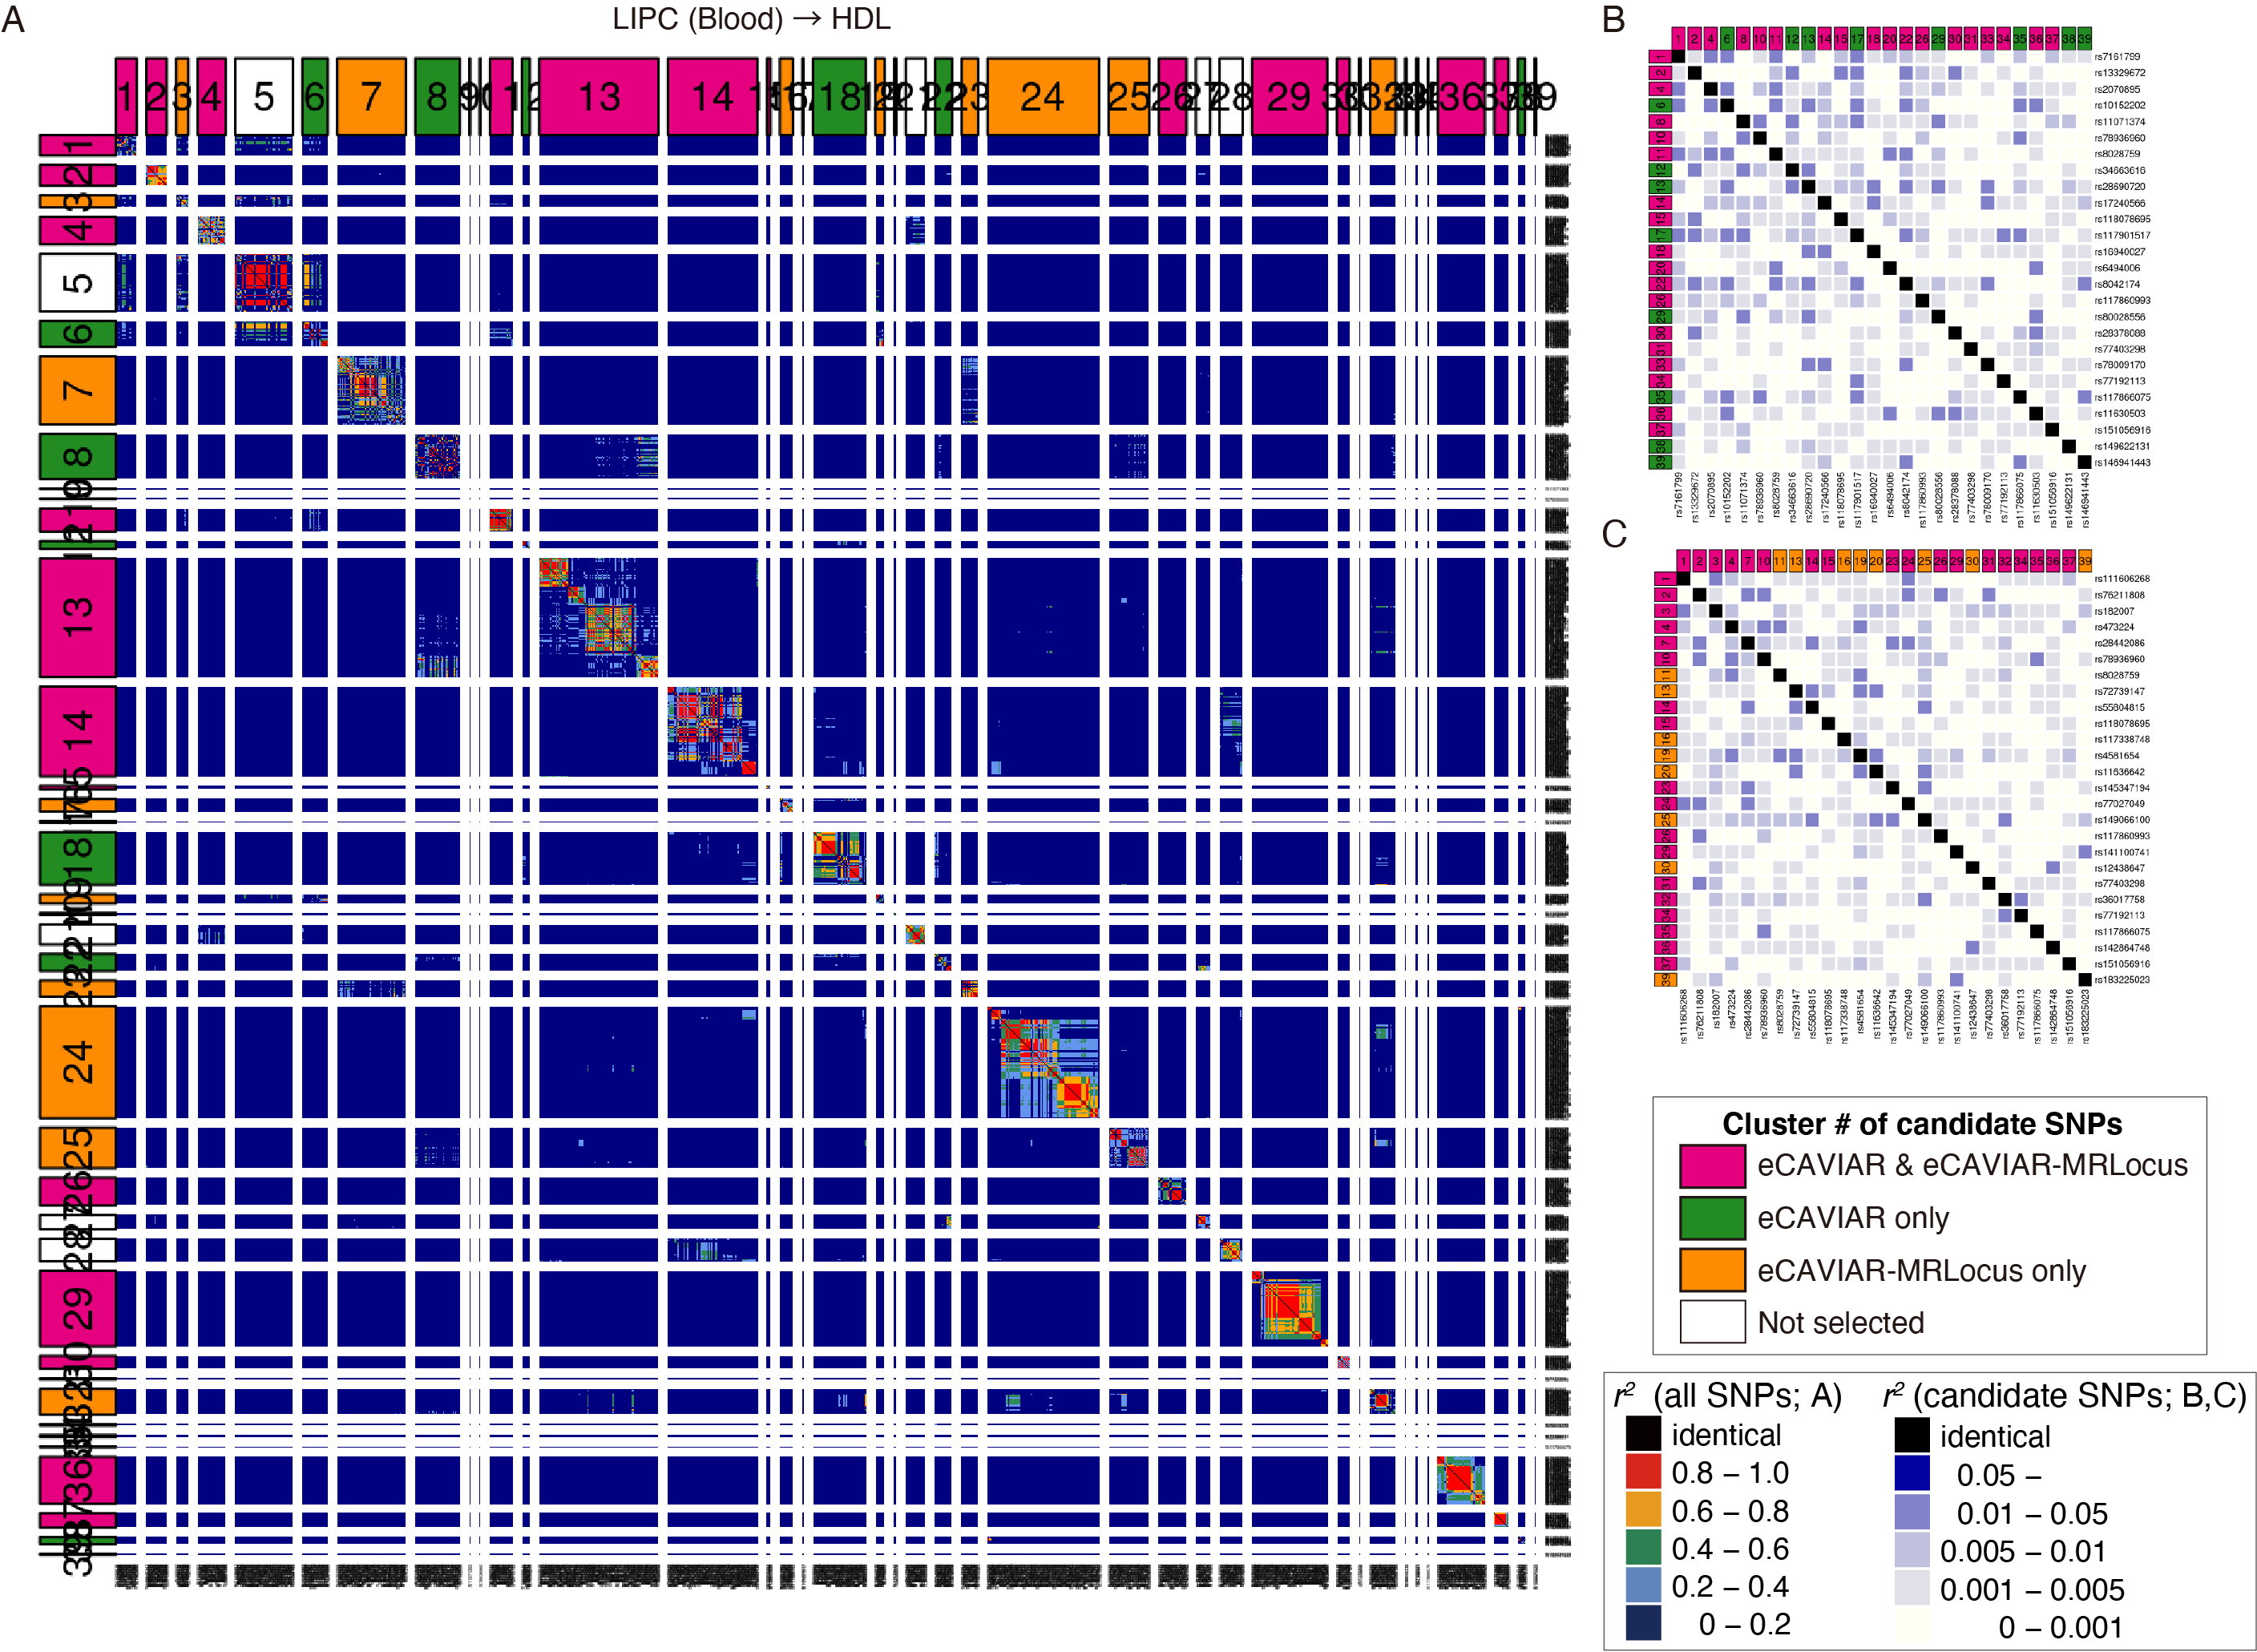
\includegraphics[width=.7\textwidth]{figs/region/heatmap_eQTLbase.Blood_LIPC_HDL.20201217.png}
%%   \caption{LD pattern across independent clusters from \emph{LIPC}
%%     eQTL (Blood) and HDL GWAS.}
%% \end{figure}

%% \begin{figure}[!ht]
%%   \centering
%%   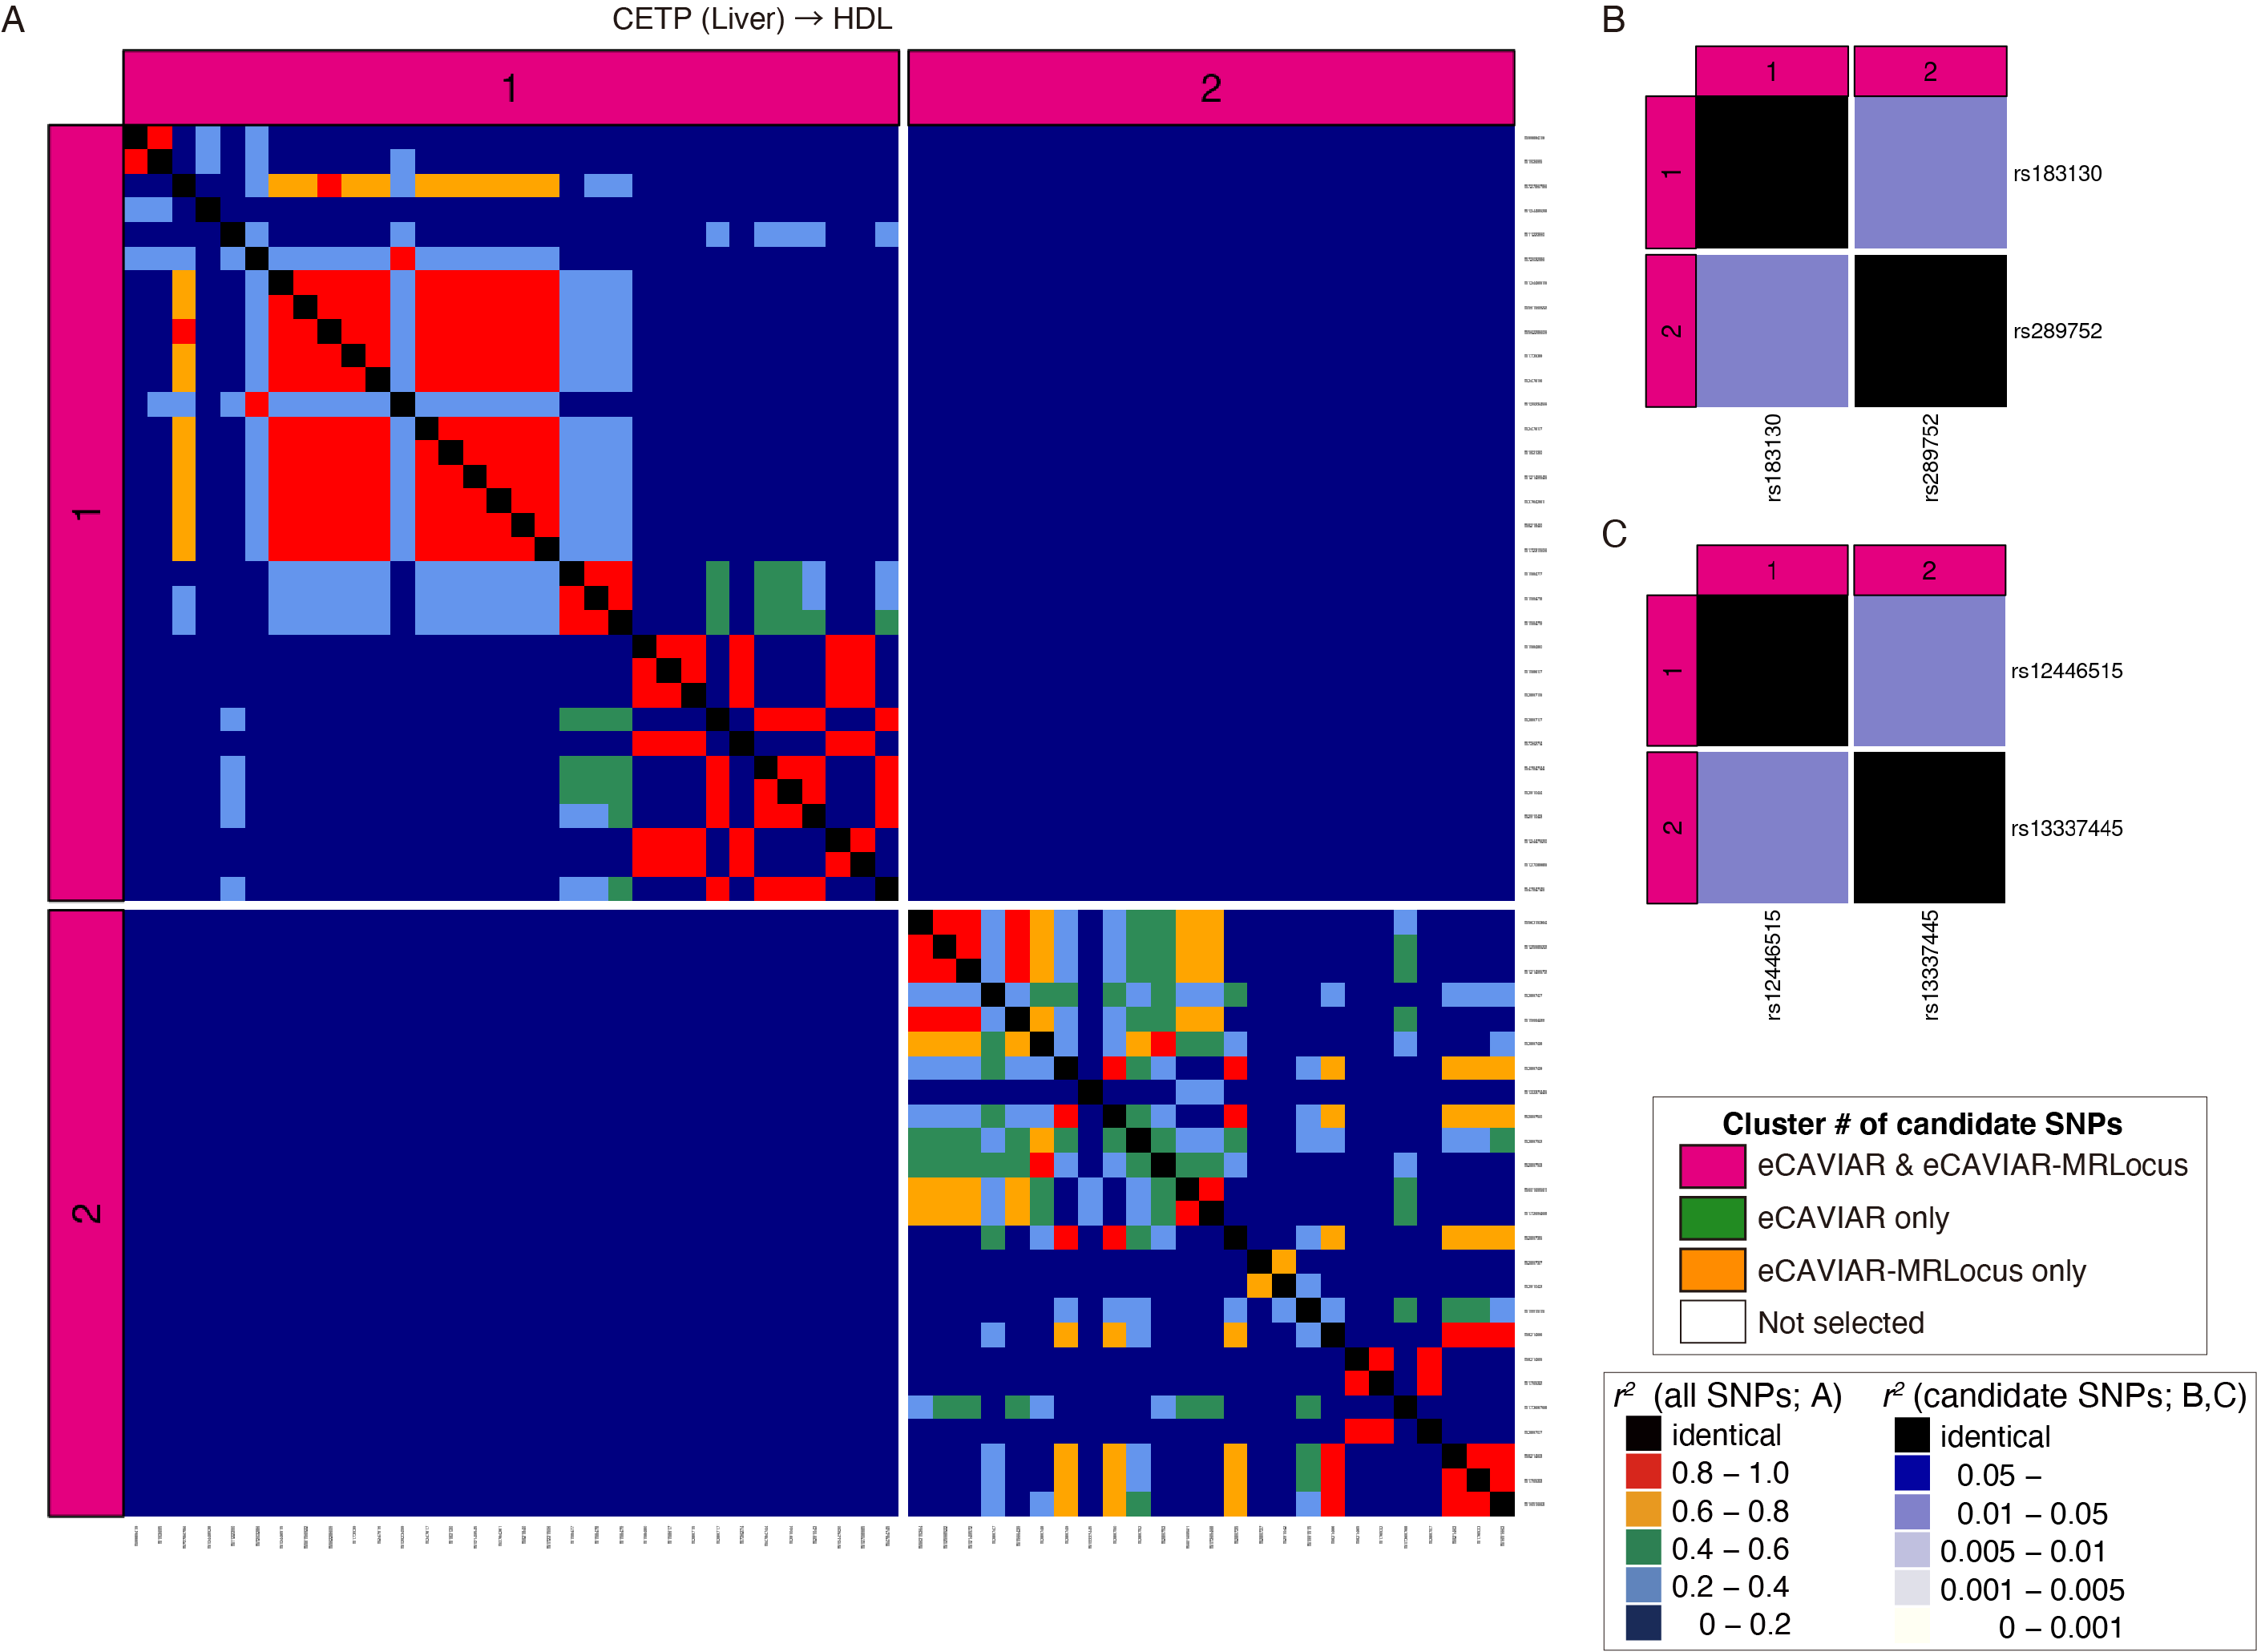
\includegraphics[width=.7\textwidth]{figs/region/heatmap_eQTLbase.Liver_CETP_HDL.20201217.png}
%%   \caption{LD pattern across independent clusters from \emph{CETP}
%%     eQTL (liver) and HDL GWAS. LD ($r^2$) between SNPs in independent
%%     clumps from \emph{CETP} in liver (columns) and HDL GWAS SNPs
%%     (rows). Color bars at the top and left represent cluster (pair) ID
%%     which is sorted by base position of index eQTL SNPs. LD was
%%     calculated to independent SNPs within 1KG EUR and colored
%%     accordingly.} 
%% \end{figure}

%% \begin{figure}[!ht]
%%   \centering
%%   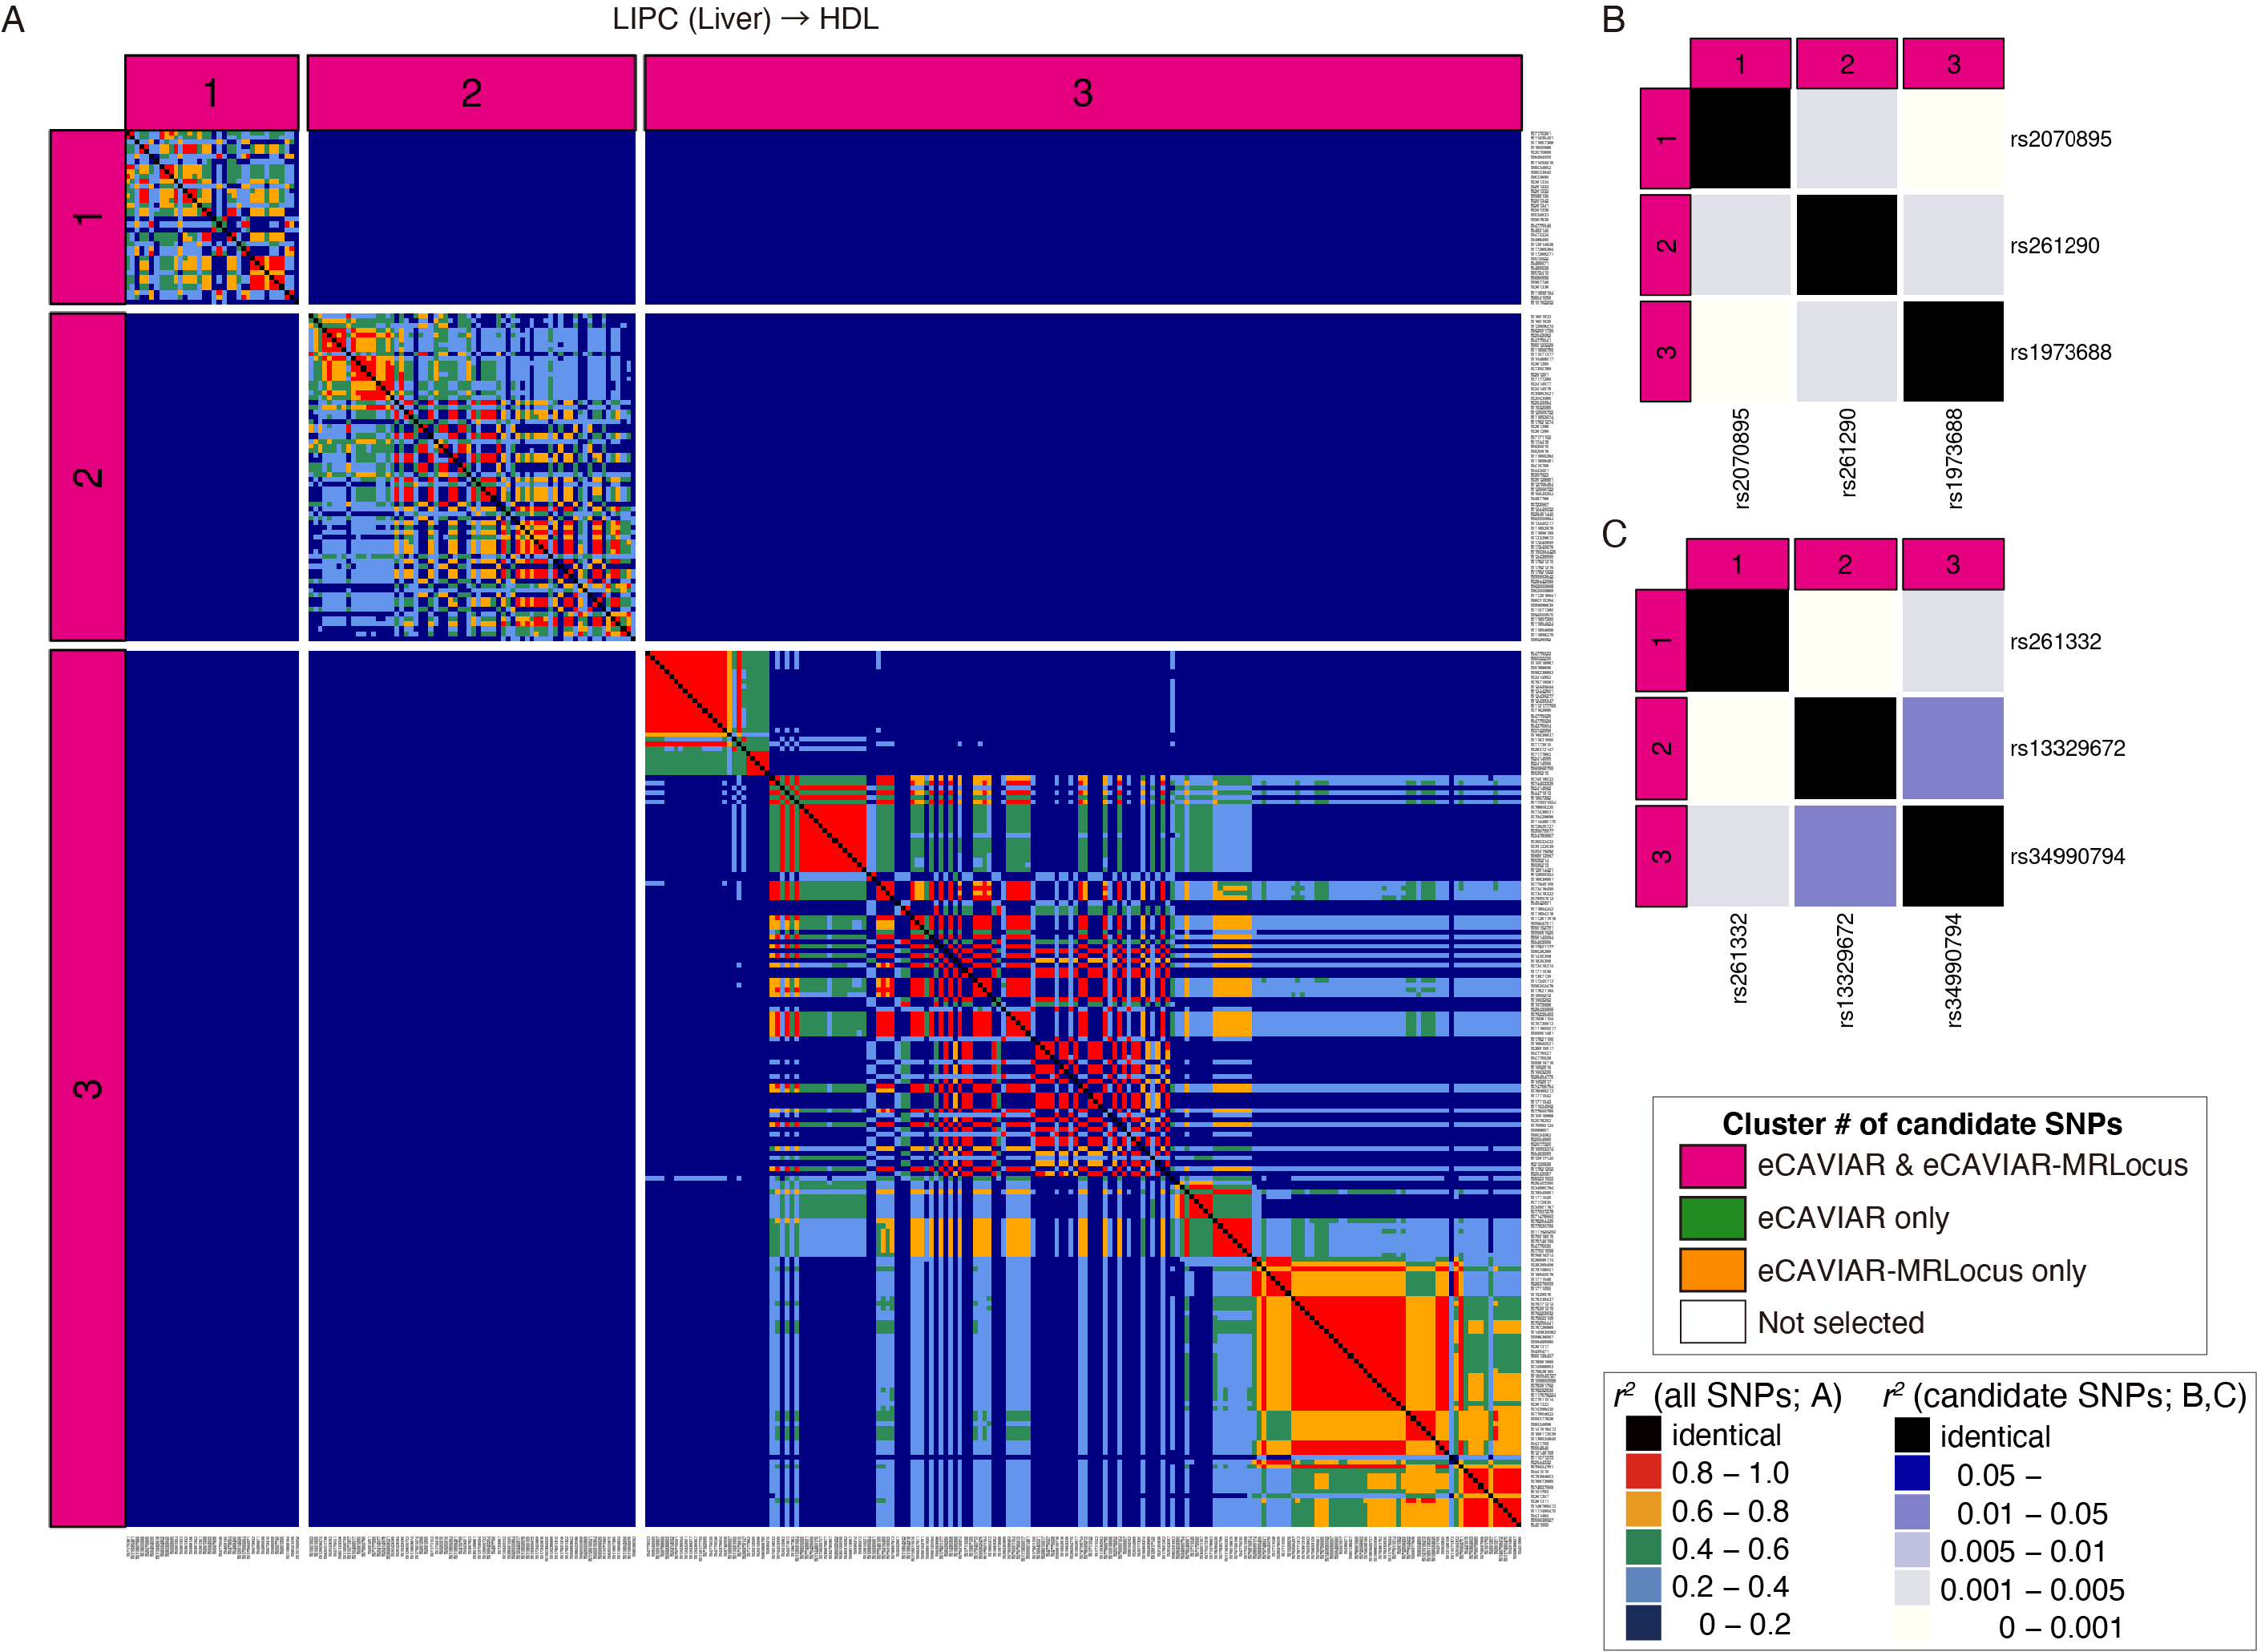
\includegraphics[width=.7\textwidth]{figs/region/heatmap_eQTLbase.Liver_LIPC_HDL.20201217.png}
%%   \caption{LD pattern across independent clusters from \emph{LIPC}
%%     eQTL (liver) and HDL GWAS. LD ($r^2$) between SNPs in independent
%%     clumps from \emph{LIPC} in liver (columns) and HDL GWAS SNPs
%%     (rows). Color bars at the top and left represent cluster (pair) ID
%%     which is sorted by base position of index eQTL SNPs. LD was
%%     calculated to independent SNPs within 1KG EUR and colored
%%     accordingly.} 
%% \end{figure}

%% \begin{figure}[!ht]
%%   \centering
%%   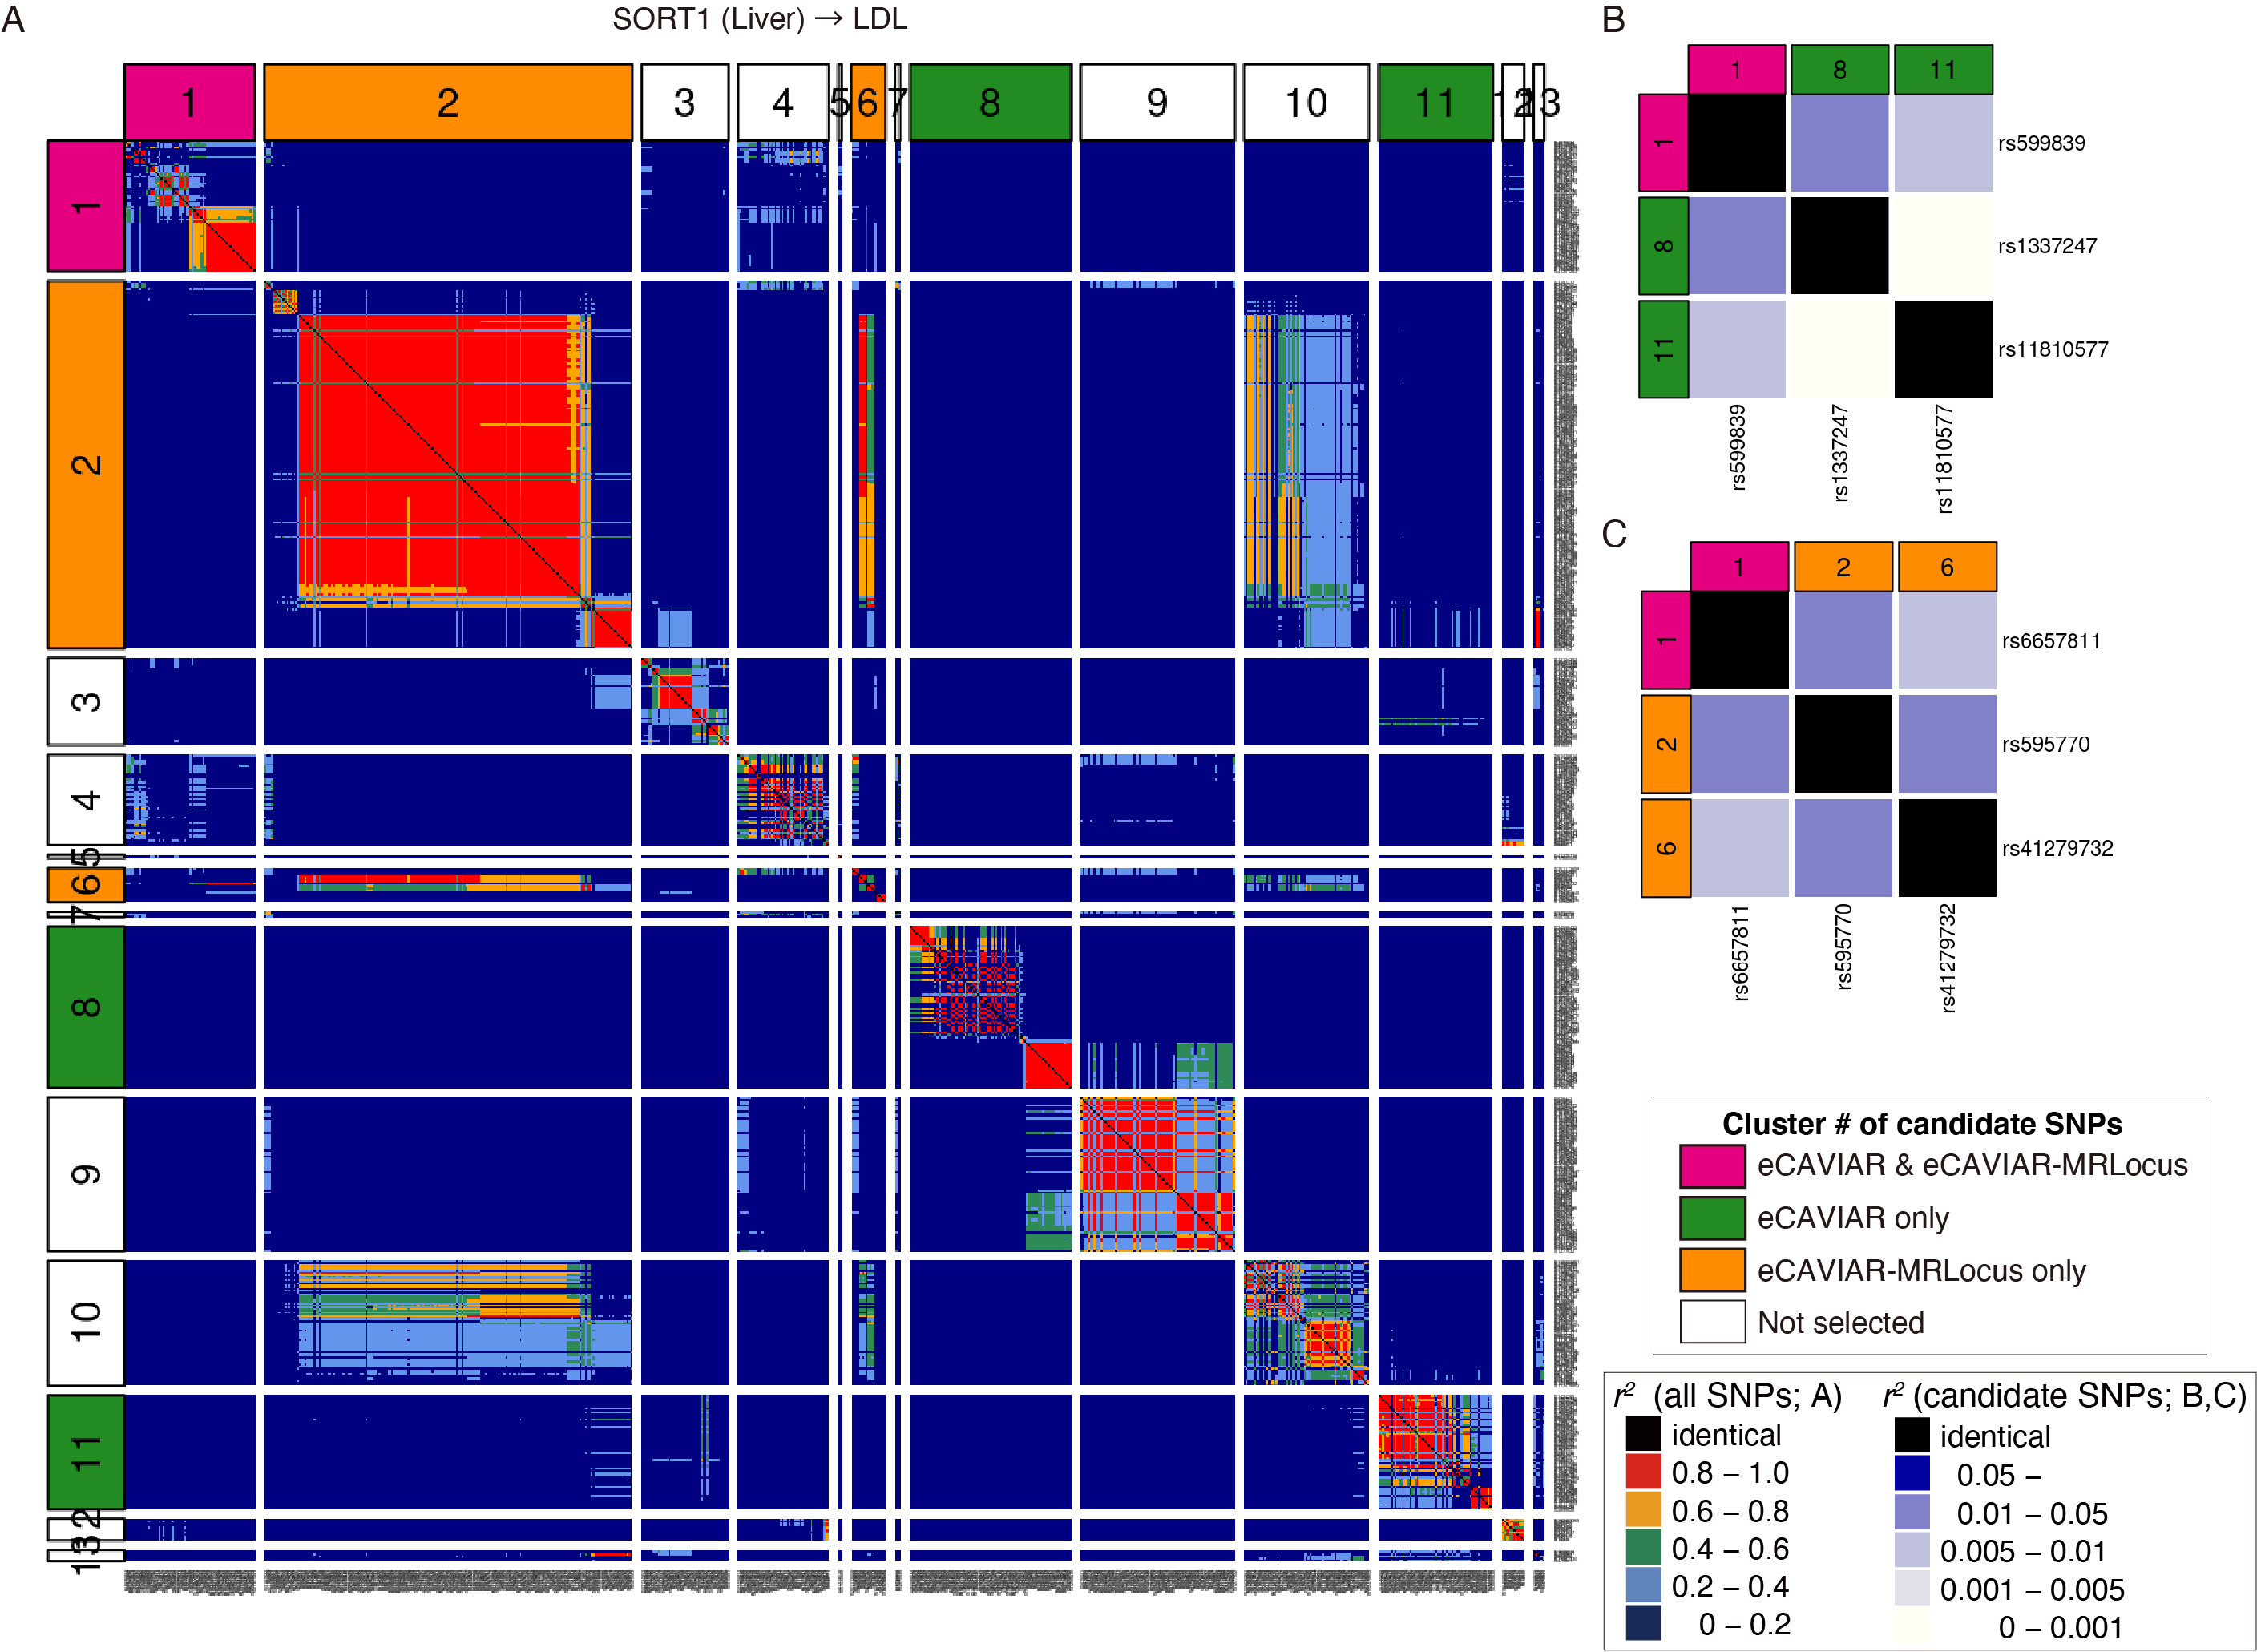
\includegraphics[width=.7\textwidth]{figs/region/heatmap_eQTLbase.Liver_SORT1_LDL.20201217.png}
%%   \caption{LD pattern across independent clusters from \emph{SORT1}
%%     eQTL (liver) and LDL GWAS. LD ($r^2$) between SNPs in independent
%%     clumps from \emph{SORT1} in liver (columns) and LDL GWAS SNPs
%%     (rows). Color bars at the top and left represent cluster (pair) ID
%%     which is sorted by base position of index eQTL SNPs. LD was
%%     calculated to independent SNPs within 1KG EUR and colored
%%     accordingly.}
%%   \label{fig:ld5}
%% \end{figure}

\begin{figure}[!ht]
  \centering
  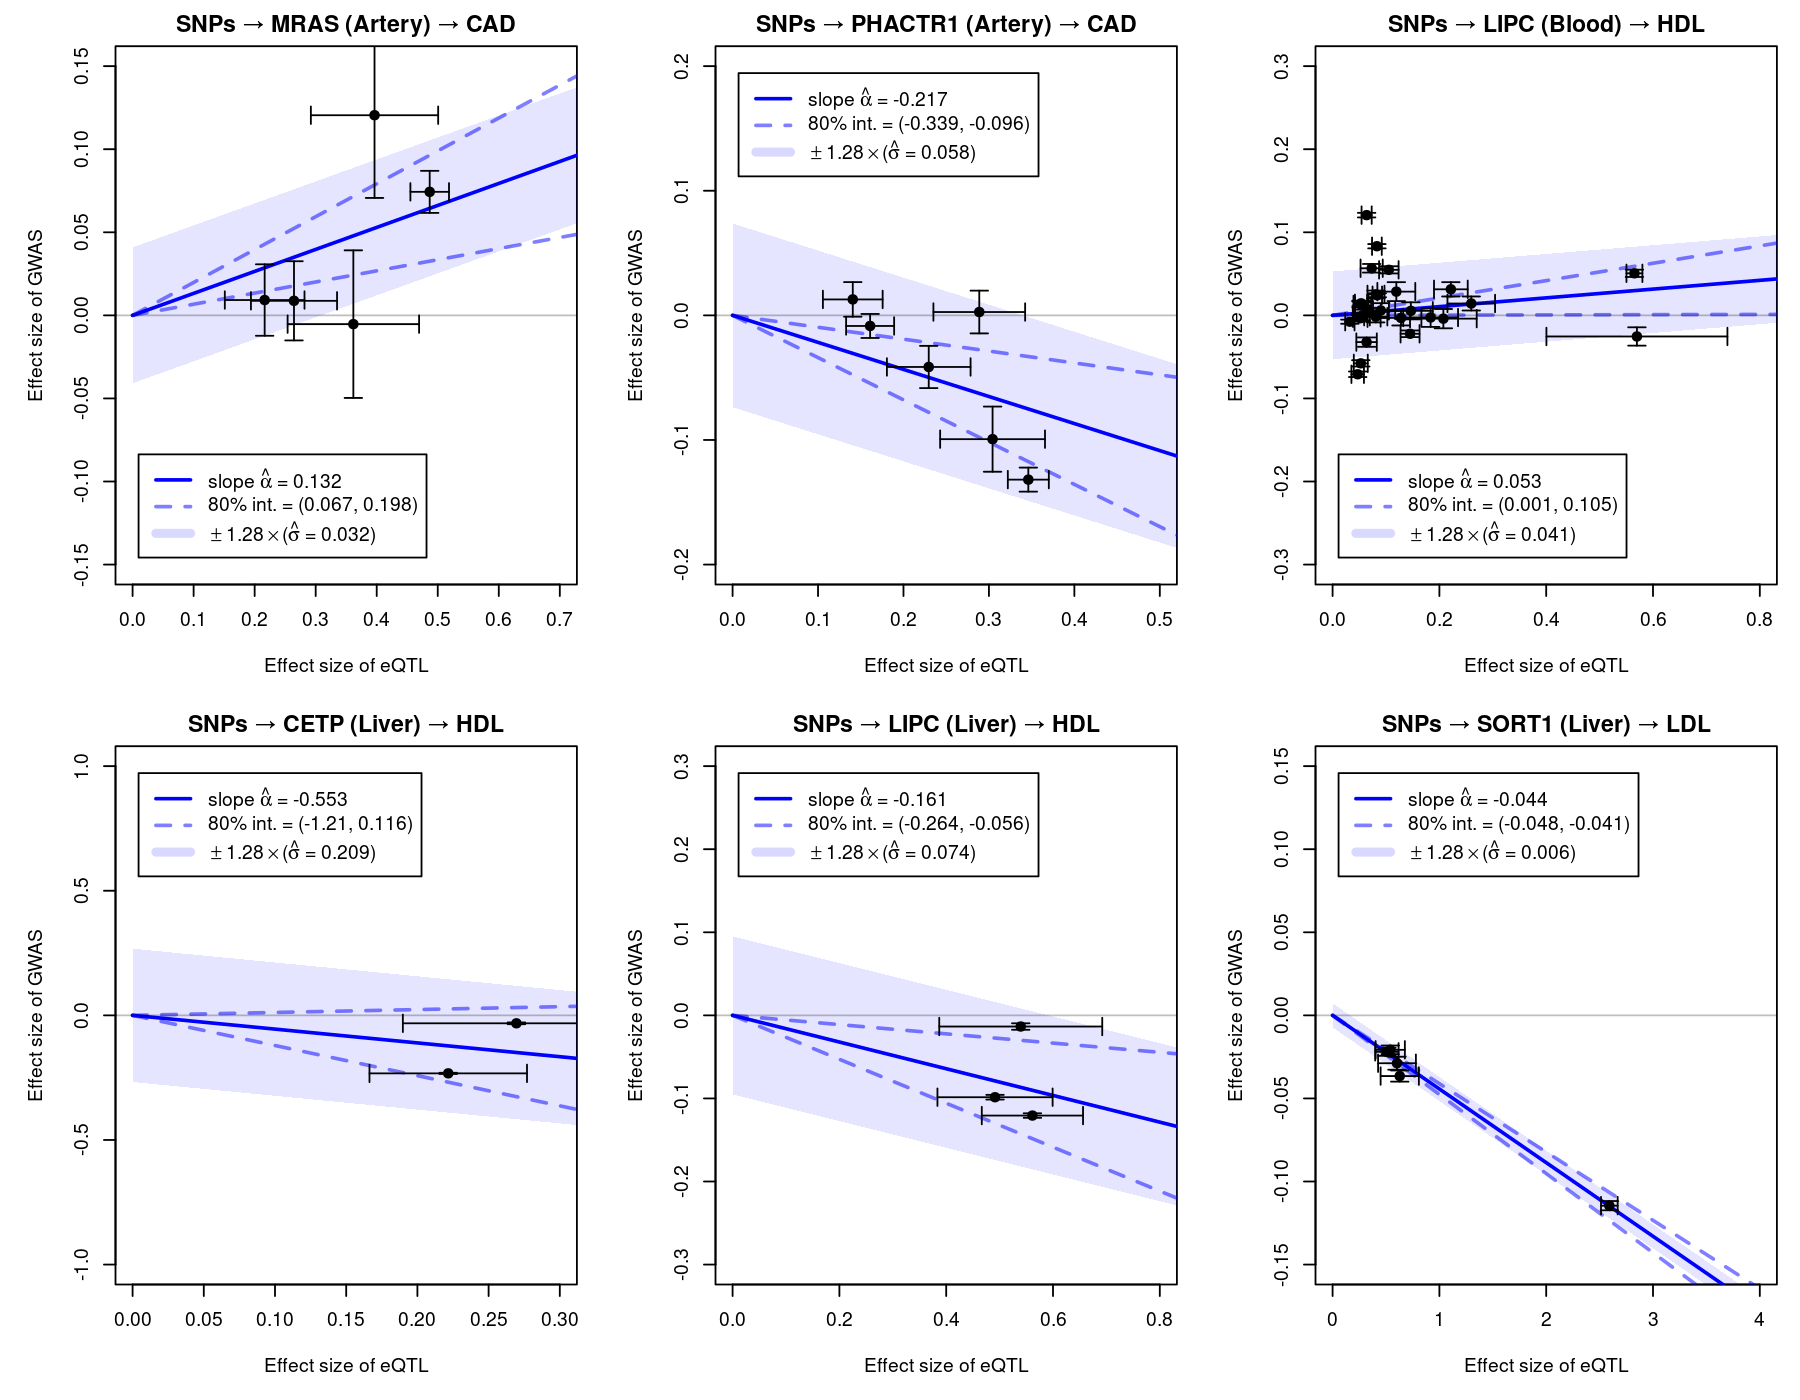
\includegraphics[width=\textwidth]{figs/real_loci_ecav-mrlocus.png}
  \caption{MRLocus plots for six gene-trait pairs, using eCAVIAR for colocalization.}
\end{figure}

\begin{figure}[!ht]
  \centering
  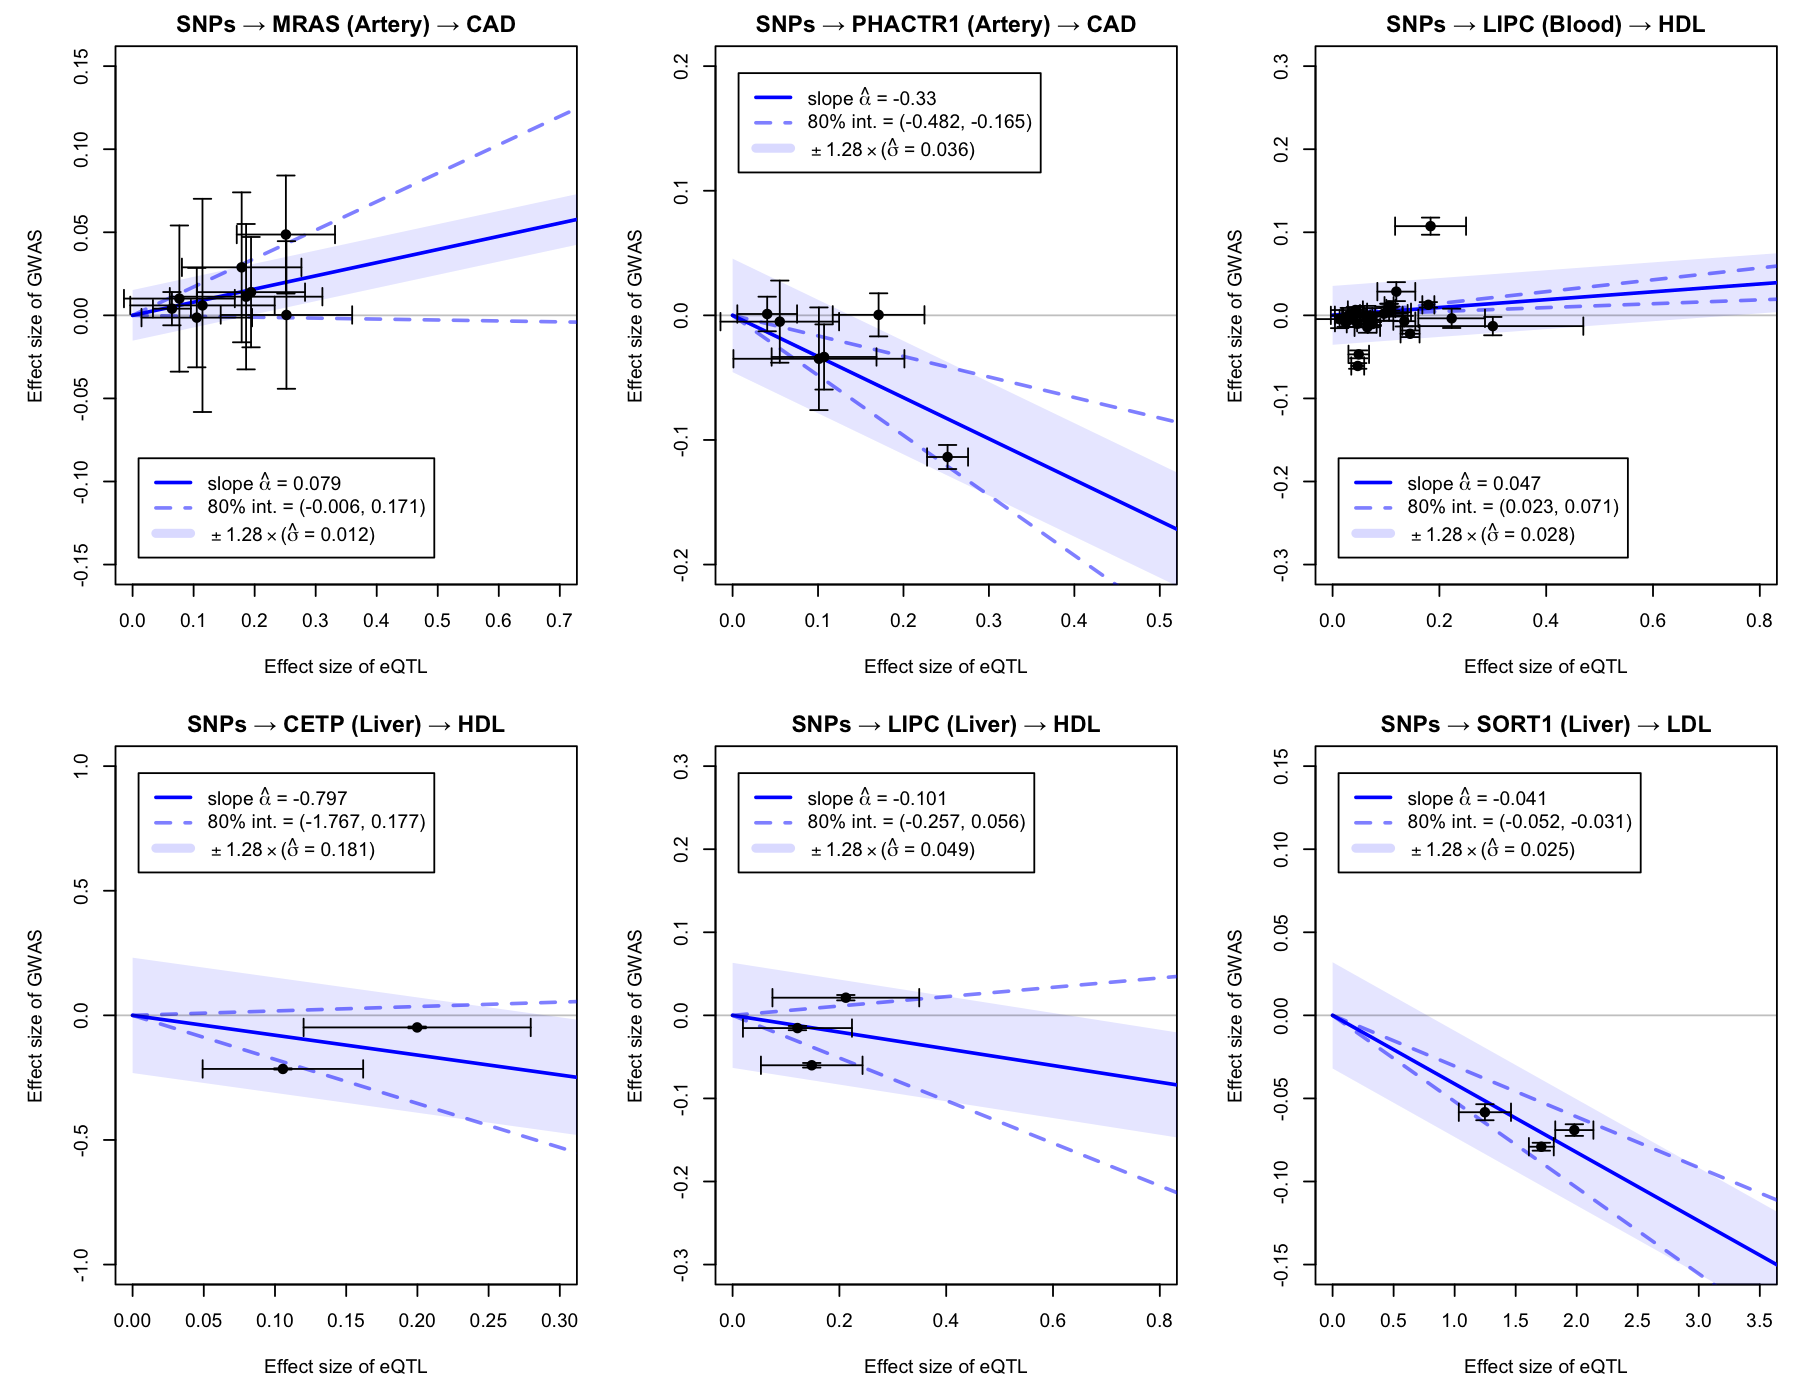
\includegraphics[width=\textwidth]{figs/real_loci_mrlocus.png}
  \caption{MRLocus plots for six gene-trait pairs, using MRLocus for colocalization.}
\end{figure}

\end{document}
